% Configuration

\def\degree{Diploma in Electrical and Computer Engineering}
\def\department{School of Electrical and Computer Engineering}


\def\supervisor{Vasilis Samoladas}
\def\assocsupervisora{Antonios Deligiannakis}
\def\assocsupervisorb{Michail G. Lagoudakis}

\documentclass[logo]{style/styles}

% Remove weird spaces in List of Figures
\newcommand*{\noaddvspace}{\renewcommand*{\addvspace}[1]{}}
\addtocontents{lof}{\protect\noaddvspace}
%%%%%%%%%%%%
% Packages
\usepackage{amstext,amssymb,amsfonts,latexsym}
\usepackage[utf8]{inputenc}
\usepackage{style/bib}
\usepackage[english]{babel}
\usepackage{lipsum}
\usepackage{csquotes}% Recommended
\usepackage{ccicons}
\usepackage{animate}
\usepackage{movie15}
\usepackage{setspace}
\usepackage{pdfpages}% for hosting full pdf docs as in appendix
\usepackage[pdftex,bookmarks=true,hidelinks]{hyperref}

%\usepackage{algorithm,algpseudocode,amsmath}
\newcommand{\var}[1]{\text{\texttt{#1}}}
\newcommand{\func}[1]{\text{\textsl{#1}}}
\makeatletter
\newcounter{phase}[algorithm]
\newlength{\phaserulewidth}
\newcommand{\setphaserulewidth}{\setlength{\phaserulewidth}}
\newcommand{\phase}[1]{%
\vspace{-1.25ex}
% Top phase rule
\Statex\leavevmode\llap{\rule{\dimexpr\labelwidth+\labelsep}{\phaserulewidth}}\rule{\linewidth}{\phaserulewidth}
\Statex\strut\refstepcounter{phase}\textit{\textbf{Phase~\thephase~--~#1 \\}}% Phase text
% Bottom phase rule
\vspace{-1.25ex}
\Statex\leavevmode\llap{\rule{\dimexpr\labelwidth+\labelsep}{\phaserulewidth}}\rule{\linewidth}{\phaserulewidth}}
\makeatother
\setphaserulewidth{.7pt}

\usepackage{geometry}
\usepackage{subcaption}

\hypersetup{
pdfauthor = {Ilias Balampanis},
pdftitle = {thesis},
colorlinks,
%    linkcolor={blue},
%    citecolor={blue}
linkcolor={black},
citecolor={black}
}

% Mathematics functions
\def\O{\mbox{O}}
\newcommand{\bsigma}{{\boldsymbol\sigma}}
\newcommand{\bepsilon}{{\boldsymbol\epsilon}}
\newcommand{\expnumber}[2]{{#1}\mathrm{e}{#2}}
\newcommand{\norm}[1]{\left\lVert#1\right\rVert}


% Setup
\newenvironment{myquote}{\list{}{\leftmargin=2.5cm\rightmargin=2.5cm}\item[]}{\endlist}

\usepackage[backend=biber]{biblatex}
\addbibresource{thesis.bib}


\usepackage{microtype}

%   Page size:
\oddsidemargin=0.2in    % really +1in
\evensidemargin=0in
\textwidth=6.1in

%\textheight=22cm
%\topmargin=-1cm

% Beautify the appendix section in ToC.
\renewcommand{\cftchappresnum}{Chapter }
\setlength{\cftchapnumwidth}{7em}% Just for this example
\let\oldappendix\appendix
\renewcommand{\appendix}{%
\oldappendix
\addtocontents{toc} % Update \cftchappresnum within the .toc
{\protect\renewcommand{\protect\cftchappresnum}{Appendix }}
}

\usepackage{amsthm}
\newtheorem{definition}{Definition}
\newtheorem{theorem}{Theorem}
\newtheorem{prop}{Proposition}

%%%%%%%%%%%%
% Start
\begin{document}

% Initial page numbers:  i, ii, iii, ...
    \renewcommand{\thepage}{\roman{page}}

% Title page
    \title{{\bf\Huge Distributed Training of Recurrent Neural Networks by FGM Protocol}}
    \author{Ilias Balampanis}

    \maketitle
    \setstretch{1.5}

% Intro pages
    \chapter*{Acknowledgments}

First and foremost, I would like to thank my mentor Vasilis Samoladas for his trust and guidance.
Besides, I am grateful for being part of this team.
Sofia, Edward, and Eftychia supported and helped me to solve my problems during this work the last year.
Furthermore, I would like to thank my friends from Chania, Stefanos, Yiorgos and Spyros, and especially Ioanna.
Together we had some amazing moments during my student life.
Last but not least, I would like to thank my family for their love, support, and constant encouragement.
    \chapter*{Abstract}

Artificial Neural Networks are appealing because they learn by example and are strongly supported by statistical and optimization theories.
The usage of recurrent neural networks as identifiers and predictors in nonlinear dynamic systems has increased significantly.
They can present a wide range of dynamics, due to feedback and are also flexible nonlinear maps.
Based on this, there is a need for distributed training on these networks, because of the enormous datasets.
One of the most known protocols for distributed training is the Geometric Monitoring protocol.
Our conviction is that this is a very expensive protocol regarding the communication of nodes.
Recently, the Functional Geometric Protocol has tested training on Convolutional Neural Networks and has had encouraging results.
The goal of this work is to test and compare these two protocols on Recurrent Neural Networks.

%\printglossary

    \newpage
    \addcontentsline{toc}{chapter}{Contents}
    \setcounter{tocdepth}{3}
    \tableofcontents
%    \listoffigures
    \listoftables


% Chapters
    \setcounter{page}{1}
    \setcounter{chapter}{0}

% Main page numbers:  1, 2, 3, ...
    \renewcommand{\thepage}{\arabic{page}}
    \setupParagraphs

    \chapter{Introduction}\label{ch:introduction}

Nowadays, deep neural networks are trained on ever-growing data corpora.
As a result, distributed training schemes are becoming increasingly important.
A major issue in distributed training is the limited communication bandwidth between contributing nodes or prohibitive communication costs in general.
Many pieces of research have made a try on distributed deep learning, but very few have considered the enormous network traffic costs that such a style requires.
Deep learning methods have proved to have strong predictive performance but on the other hand, a complex learning process.
Opportunely, the training of artificial neural networks uses algorithms like Gradient Descent decreasing their loss, a fact that leads to convenience to distribute their learning procedure.
In this work, we focus on distributing the learning process of Recurrent Neural Networks, while minimizing the communication of the remote sites.

\section{Related Work and Motivation}\label{sec:related-work-and-motivation}

The first tries for Distributed Machine Learning (DML) or Deep Learning were done by the parameter server method~\cite{li_scaling_2014}.
This structure of this method has nodes and a parameter server.
The central idea is when some batches of data or some real training time have passed, nodes synchronize with the server sending their parameters.
Then, the server aggregates all these model parameters and send back to nodes the fresh one to continue the learning process.

In 2019, Konidaris~\cite{konidaris_distributed_2019} used the GM~\cite{sharfman_geometric_2007}~\cite{sharfman_aggregate_2007}
and the FGM~\cite{garofalakis_sketch-based_2013}~\cite{garofalakis_distributed_nodate}~\cite{samoladas_functional_nodate} to train one other architecture of Artificial Neural Networks, the Convolutional Neural Networks.
The work had unbelievable results regarding the gap of the network cost between the two methods.
So, there I found the motivation to use these two methods, this time to train an architecture that comprises Recurrent Neural Networks.
Besides, while searching for my diploma thesis subject, I do not found a lot of works on distributed training of RNNs.
Making work with successful results translates to a valuable source for other people in the Machine Learning community.

\section{Contribution}\label{sec:contribution}

This work aims to provide a comparison of two methods for a distributed training process of Recurrent Neural Networks.
The comparison is about the network cost of these two methods.
I focus on two supervised learning problems, Classification and Natural Language Processing, using a subset of the RNN architecture, the Long-Short Term Memory Networks as learning models.
The distributed learning process will be achieved by two geometric monitoring methods, the GM and the FGM\@.

\section{Thesis Overview}\label{sec:thesis-overview}

This section summarizes the structure of this diploma thesis.

\textbf{Chapter~\ref{ch:theoretical-background}} presents the background you need to understand the meanings of this work.
At first, section \textbf{\ref{sec:machine-learning}} refers to Machine Learning Paradigms and Deep Learning.
It makes a further reference to Recurrent Neural Networks because my Deep Learning model is based on there.
Finally, section \textbf{\ref{sec:geometric-monitoring-methods}} introduces the two Geometric Monitoring methods which I have implemented and compared each other.

\textbf{Chapter~\ref{ch:implementation}} presents the tools that helped me to implement the above algorithms.
It also presents the structure and setup of the Deep Learning model.
Lastly, explains in detail the implementation by giving some pseudocodes to make it easier to understand.

\textbf{Chapter~\ref{ch:experimental-results}}, explains the results that came off from the experimental phase.

\textbf{Chapter~\ref{ch:conclusions}}, concludes this work as well as proposes some ideas for further research in the future.

In the end, \textbf{Appendix~\ref{ch:abbreviations}} you can find the abbreviations I have used in my text,
while \textbf{Appendix~\ref{ch:detailed-experimental-results}} provides the tables with the numerical data that resulted from the experimental phase.
    \subsection{Machine Learning}\label{subsec:machine-learning}

\begin{frame}{Machine Learning (ML)}
    \setbeamertemplate{itemize items}[square]
    \begin{itemize}
        \item{It is computational process for improving performance based on experience.}
        \vspace{0.4cm}
        \item{ML is a subfield of Artificial Intelligence (AI) and is primarily related to Data Analysis.}
        \vspace{0.4cm}
        \item{ML approaches are commonly divided into three ($3$) broad categories:
        \setbeamertemplate{enumerate items}[circle]
        \begin{enumerate}
            \item Supervised Learning %(correct answers for each training point)
            \item Unsupervised Learning %("just make sense of the data")
            \item Reinforcement Learning %(reward sequence, no correct answers)
        \end{enumerate}}
    \end{itemize}
\end{frame}

\begin{frame}{Neural Networks (NN)}
    \setbeamertemplate{itemize items}[square]
    \begin{itemize}
        \item{A dominant class of ML algorithms.}
        \vspace{0.2cm}
        \item{ML with NN $\implies$ Deep Learning (DL)}
        \vspace{0.2cm}
        \item{Inspired by the neurophysiological experiments conducted by Hubel \& Wiesel in 1962.}
        \vspace{0.2cm}
        \item{Can approach highly complex functions and decision regions.}
        \vspace{0.2cm}
        \item[]{
        \begin{figure}[H]
            \centering
            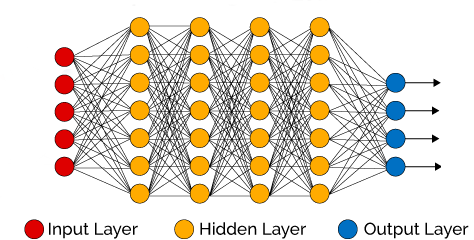
\includegraphics[width=8cm,height=3.8cm]{images/dnn.png}
            \caption{a Deep Neural Network.}
            \label{fig:dnn}
        \end{figure}}
    \end{itemize}
\end{frame}

\begin{frame}{NN learning process}
    \setbeamertemplate{itemize items}[square]
    \begin{itemize}
        \item{Assume a set $D=\{(x,y)\:|\:x\in\mathbb{R}^n,y\in\mathbb{N}\}$ of training data points.}
        \vspace{0.3cm}
        \item{A NN is a non-linear function $f$ parameterized by $w\in\mathbb{R}^d$.}
        \vspace{0.3cm}
        \item{Consider a globally continuous and differentiable \textbf{loss function} $\mathcal{L}:\mathcal{F}\times\mathcal{X}\times\mathcal{Y}\rightarrow\mathbb{R}_+$.}
        \vspace{0.3cm}
        \item{Training is performed by the mini-batch Gradient Descent (GD) algorithm
        \begin{itemize}
            \item[]{
            \begin{algorithm}[H]
                \begin{algorithmic}[1]
                    \WHILE{does not \emph{converge}}
                    \STATE \textbf{pick} randomly a mini-batch $\beta=\{(x_1,y_1),\dots,(x_{|\beta|},y_{|\beta|})\} \subset D$
                    \STATE \textbf{update} $w_{t+1}=w_t-\alpha\frac{1}{|\beta|}\sum_{i=1}^{|\beta|}\nabla_w\mathcal{L}(y_i,\hat{y_i})$
                    \ENDWHILE
                \end{algorithmic}
                \label{alg:gd}
            \end{algorithm}
            }
        \end{itemize}
        with $|\beta| \ll |D|$.}
    \end{itemize}
\end{frame}

\begin{frame}{Recurrent Neural Networks (RNN)}
    \setbeamertemplate{itemize items}[square]
    \begin{itemize}
        \item{Introduced by David Rumelhart in 1986.}
        \vspace{0.2cm}
        \item{Can handle sequential data.}
        \vspace{0.2cm}
        \item{Considers the current input and also the previously received inputs.}
        \vspace{0.2cm}
        \item{Can memorize previous inputs due to its internal memory.}
        \vspace{0.2cm}
        \item[]{
        \begin{figure}[H]
            \centering
            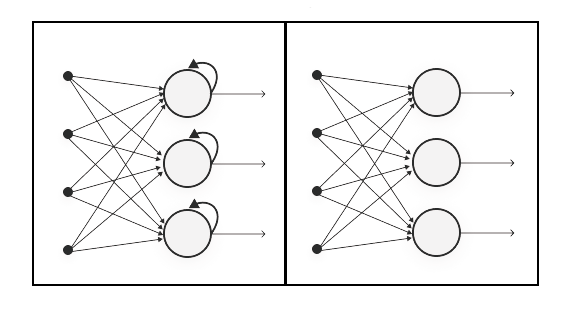
\includegraphics[width=7cm,height=3.5cm]{images/rnn-vs-fnn.png}
            \caption{a Recurrent Neural Network vs a Feed-forward one.}
            \label{fig:rnn-vs-fnn}
        \end{figure}
        }
    \end{itemize}
\end{frame}

\begin{frame}{LSTM Networks}
    \begin{columns}
        \column{0.55\textwidth}
        \setbeamertemplate{itemize items}[square]
        \begin{itemize}
            \item{LSTM for Long Short Term Memory.}
            \vspace{0.2cm}
            \item{Not fundamentally different\\from RNN.}
            \vspace{0.2cm}
            \item{Use different functions to\\compute hidden state.}
            \vspace{0.2cm}
            \item{Cells decide what to keep in memory.}
            \vspace{0.2cm}
            \item{Very effective in capturing\\long term dependencies.}
        \end{itemize}
        \column{0.45\textwidth}
        \begin{figure}
            \subfigure[\tiny{The repeating module in a standard RNN contains a single layer.}]{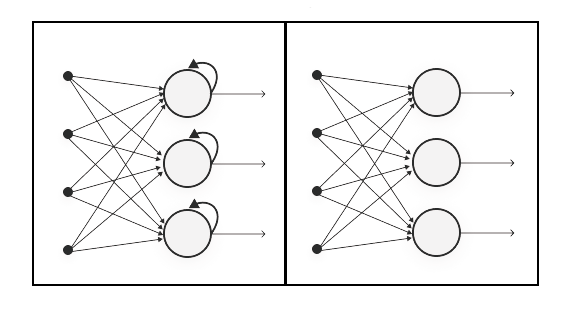
\includegraphics[width=3.8cm,height=2.5cm]{images/rnn.png}}
            \subfigure[\tiny{The repeating module in an LSTM contains four interacting layers.}]{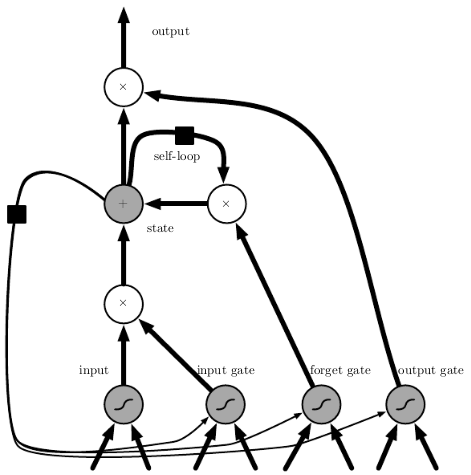
\includegraphics[width=3.8cm,height=2.5cm]{images/lstm.png}}
            \label{fig:rnn-vs-lstm}
        \end{figure}
    \end{columns}
\end{frame}

\subsection{Distributed Deep Learning}\label{subsec:distributed-deep-learning}

\begin{frame}{Network Architecture}
    \begin{columns}
        \column{0.5\textwidth}
        \setbeamertemplate{itemize items}[square]
        \begin{itemize}
            \item{A \textbf{star network} topology with
            \setbeamertemplate{itemize items}[circle]
            \begin{itemize}
                \item a \emph{parameter server}
                \item $n$ remote \emph{workers}
            \end{itemize}}
            \vspace{0.2cm}
            \item{Each worker $i \in [\,1,n]\,$ has a chunk $D_i$ of the whole training set $D$.}
            \vspace{0.2cm}
            \item{Each worker has a \textbf{replica} of the DL model.}
        \end{itemize}
        \column{0.5\textwidth}
        \begin{figure}
            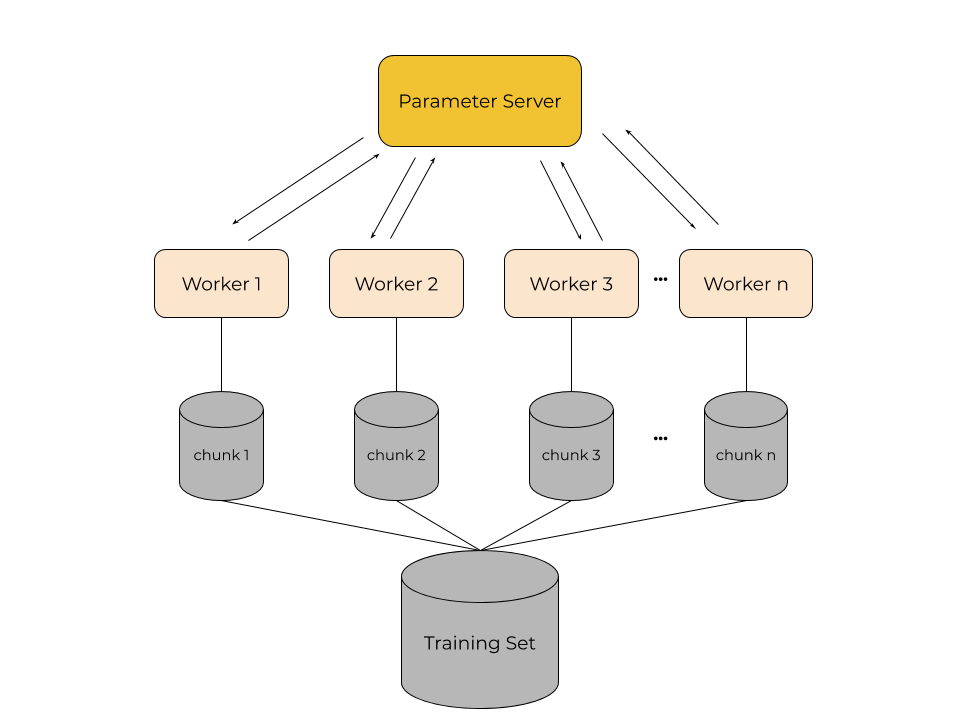
\includegraphics[width=8.5cm,height=6cm,center]{images/parameter-server.png}\label{fig:param-server}
        \end{figure}
    \end{columns}
\end{frame}

\begin{frame}{Parameter Server (PS) model}
    \setbeamertemplate{itemize items}[square]
    \begin{itemize}
        \item{The most known model for distributed DL.}
        \vspace{0.2}
        \item{\textbf{Pseudo algorithm}}
        \vspace{0.1}
        \item[]{
        \begin{algorithm}[H]
            \begin{algorithmic}[1]
                \STATE The PS initializes the parameters of the DL model.
                \STATE The PS broadcasts the model parameters to each worker.
                \STATE Each worker fits a mini-batch, taken from its chunk, using the mini-batch GD algorithm.
                \STATE When \textbf{step 3} is done, all workers send their model parameters\\to the PS where the aggregation takes place.
                \STATE While each chunk is not empty, go to \textbf{step 2}, otherwise \textbf{all done}.
            \end{algorithmic}
            \label{alg:param-server}
        \end{algorithm}
        }
    \end{itemize}
\end{frame}
    \subsection{Deep Learning using Functional Geometric Monitoring (FGM) protocol}\label{subsec:deep-learning-using-fgm-protocol}

\begin{frame}{Definitions}
    \begin{block}{Definition (Safe function for admissible region $A$)}
        A function $\phi :\mathbb{R}^d\rightarrow \mathbb{R}$ such that, for every $n$, and every $\pmb{X}_i$, i \in [\,1,n]\,\\
        \vspace{0.1cm}
        \begin{center}
            $\sum_{i=1}^n\phi (\pmb{X}_i) \leq 0$\hspace{0.4cm}$\Longrightarrow$\hspace{0.4cm}$\frac{1}{n}\sum_{i=1}^n\pmb{X}_i\in A$
        \end{center}
        We can call this function as \textbf{'spherical cap'}.
    \end{block}
    \vspace{0.4cm}
    \begin{columns}
        \column{0.65\textwidth}
        \begin{itemize}
            \item[]{The FGM protocol [Samoladas et al. 2018] monitors the condition $\sum_{i=1}^n\phi (\pmb{X}_i) \leq 0$.}
        \end{itemize}
        \column{0.35\textwidth}
        \begin{tikzpicture}
            \filldraw[color=red!60, fill=gray!50, fill opacity=0.3, very thick](0,0) circle (2);
            \coordinate (E) at (0,0);
            \coordinate (u1) at (0.3,-0.5);
            \coordinate (u2) at (-1.4,1.0);
            \coordinate (u3) at (-1.2,-1.1);
            \draw [fill] (E) circle (0.2em) node [anchor=south] {$\vec{E}$};
            \draw [->,thin] (-2,-2)--(u1)  node [anchor=north]{$\vec{X}_1$};
            \draw [->,thin] (-2,-2)--(u2) node [anchor=south west] {$\vec{X}_2$};
            \draw [->,thin] (-2,-2)--(u3) node [anchor=south]
            {$\vec{X}_3$};
            \coordinate (x) at (-0.76,-0.2);
            \draw [blue,dashed] (E)--(x);
            \draw [fill] (x) circle (0.2em) node [anchor=south] {$\vec{W}$};
            \draw [red,dashed] (E)--(2,0) node [pos=0.5, anchor=south] {$\sqrt{T}$};
        \end{tikzpicture}
    \end{columns}
\end{frame}

\begin{frame}{Correspondence with GM protocol}
    \setbeamertemplate{itemize items}[circle]
    \begin{itemize}
        \item{The \textbf{admissible region} in GM protocol (M. Kamp) is the \textbf{convex set}
        \newline
        \begin{center}
            $A=\{\pmb{X}_i\in\mathbb{R}^d\:\:|\:\:||\pmb{X}_i-\pmb{E}||_2^2 - T \leq 0\}$
        \end{center}
        }
        \vspace{0.4cm}
        \item{Samoladas et al. constructed the concave function $\phi:\mathbb{R}^d\rightarrow\mathbb{R}$ that is safe for $A$ as
        \newline
        \begin{center}
            $\phi(\pmb{X_i},\pmb{E}) = \max\{-T||\pmb{E}|| - \pmb{X_i}\frac{\pmb{E}}{\pmb{||E||}}, ||\pmb{X_i}+\pmb{E}|| - (1+T)||\pmb{E}||\}$
        \end{center}
        }
        \vspace{0.4cm}
        \item{Finally, the coordinator monitors the condition,
        \newline
        \begin{center}
            $\sum_{i=1}^n\phi(\pmb{X}_i,\pmb{E}) \leq 0$
        \end{center}
        }
    \end{itemize}
\end{frame}

\begin{frame}{The FGM Protocol (1)}
    \setbeamertemplate{itemize items}[circle]
    \begin{itemize}
        \item{At the \textbf{beginning} of a round,
        \vspace{0.2cm}
        \setbeamertemplate{itemize items}[square]
        \begin{itemize}
            \item{The coordinator knows the model parameters from all workers $\pmb{W}_i$.}
            \vspace{0.3cm}
            \item{The coordinator ships the estimate $\pmb{E}$ to all workers.}
            \vspace{0.3cm}
            \item{Each site calculates $\phi$ from $\pmb{E}$.}
            \vspace{0.3cm}
            \item{Each site initializes $\pmb{W}_i=\pmb{E}$.}
        \end{itemize}
        }
    \end{itemize}
\end{frame}

\begin{frame}{The FGM Protocol (2)}
    \setbeamertemplate{itemize items}[circle]
    \begin{itemize}
        \item{\textbf{During} a round,
        \vspace{0.2cm}
        \setbeamertemplate{itemize items}[square]
        \begin{itemize}
            \item{Each worker updates $\pmb{W}_i$ by fitting a batch of samples.}
            \vspace{0.3cm}
            \item{Next, each worker calculates its drift vector $\pmb{X}_i$ and also checks\\the \textbf{local violation} condition.}
            \vspace{0.3cm}
            \item{If a \textbf{local violation} occurs, the coordinator decides if a new round or a new subround begins.}
        \end{itemize}
        }
    \end{itemize}
\end{frame}

\begin{frame}{The FGM Protocol (3)}
    \setbeamertemplate{itemize items}[circle]
    \begin{itemize}
        \item{At the \textbf{end} of a round,
        \vspace{0.2cm}
        \setbeamertemplate{itemize items}[square]
        \begin{itemize}
            \item{The coordinator receives from each worker the current $\pmb{X}_i$.}
            \vspace{0.3cm}
            \item{The coordinator calculates the new estimate ($\pmb{E}$) and quantum ($\pmb{\theta}$).}
        \end{itemize}
        }
    \end{itemize}
\end{frame}

\begin{frame}{Conditions}
    \setbeamertemplate{itemize items}[circle]
    \begin{itemize}
        \item{The coordinator monitors the following condition,\\
        \begin{center}
            $\psi = \sum_{i=1}^n\phi(\pmb{X}_i,\pmb{E}) \leq 0$
        \end{center}
        }
        \vspace{0.3cm}
        \item{If $\psi\approx0$, the round ends and a new begins, otherwise a new subround begins.}
        \vspace{0.3cm}
        \item{The \textbf{goal} of each subround is to check the condition $\psi \leq 0$ coarsely, with a precision of $\theta = -\frac{\psi}{2n}$ (\emph{quantum}), achieving
        this with as little communication as possible.}
    \end{itemize}
\end{frame}
    \subsection{Protocols Comparison}\label{subsec:protocols-comparison}

\begin{frame}{Experiments Setup}
    \setbeamertemplate{itemize items}[circle]
    \begin{itemize}
        \item{\textbf{Quantities} that we care for
        \setbeamertemplate{itemize items}[square]
        \begin{itemize}
            \item{ML model prediction \textbf{accuracy}}
            \item{number of \textbf{rounds} of each protocol}
            \item{network \textbf{traffic} in bytes that each protocol needed to perform}
        \end{itemize}
        }
        \vspace{0.2cm}
        \item{The experiments conducted for \textbf{various}
        \setbeamertemplate{itemize items}[square]
        \begin{itemize}
            \item{thresholds ($\pmb{T}$)}
            \item{mini-batch sizes ($\pmb{|\beta|}$)}
            \item{number of workers ($\pmb{n}$)}
        \end{itemize}
        }
        \vspace{0.2cm}
        \item{Both datasets cut into $\pmb{n}$ chunks.}
        \vspace{0.2cm}
        \item{The working load allocated \textbf{uniformly} to each worker.}
    \end{itemize}
\end{frame}

\begin{frame}{Machine Learning Problems (1)}
    \setbeamertemplate{itemize items}[circle]
    \begin{itemize}
        \item{We compare the two protocols in \textbf{two} distinct ML problems using the \textbf{same safe function} (spherical cap).}
        \vspace{0.3cm}
        \item{\textbf{Problem 1} - Classification
        \vspace{0.1cm}
        \setbeamertemplate{itemize items}[square]
        \begin{itemize}
            \item{\textbf{Dataset:} San Francisco Crime Classification (SFCC)}
            \vspace{0.1cm}
            \item{\textbf{Features:} $9$}
            \vspace{0.1cm}
            \item{\textbf{Classes:} $39$}
            \vspace{0.1cm}
            \item{\textbf{Dataset size:} $878,049$ data points}
            \vspace{0.1cm}
            \item{The \textbf{goal} is to predict the category of crime that occurred, given the time and location and the rest of
            variables.}
        \end{itemize}
        }
    \end{itemize}
\end{frame}

\begin{frame}{Machine Learning Problems (2)}
    \setbeamertemplate{itemize items}[circle]
    \begin{itemize}
        \item{\textbf{Problem 2} - Natural Language Processing (NLP)
        \vspace{0.1cm}
        \setbeamertemplate{itemize items}[square]
        \begin{itemize}
            \item{\textbf{Dataset:} Amazon Fine Food Reviews (AFFR)}
            \vspace{0.2cm}
            \item{\textbf{Max input words:} $200$}
            \vspace{0.2cm}
            \item{\textbf{Classes:} $2$}
            \vspace{0.2cm}
            \item{\textbf{Dataset size:} $568,454$ data points}
            \vspace{0.2cm}
            \item{The \textbf{goal} is to predict if the given review is positive or negative\\\textbf{(Sentiment Analysis)}.}
        \end{itemize}
        }
    \end{itemize}
\end{frame}

\begin{frame}{Results (1) - Changing the threshold ($\pmb{T}$)}
%    \begin{itemize}
%        \item[]{A comment.}
%    \end{itemize}
%    \vspace{-0.4cm}
    \begin{figure}
        \subfigure{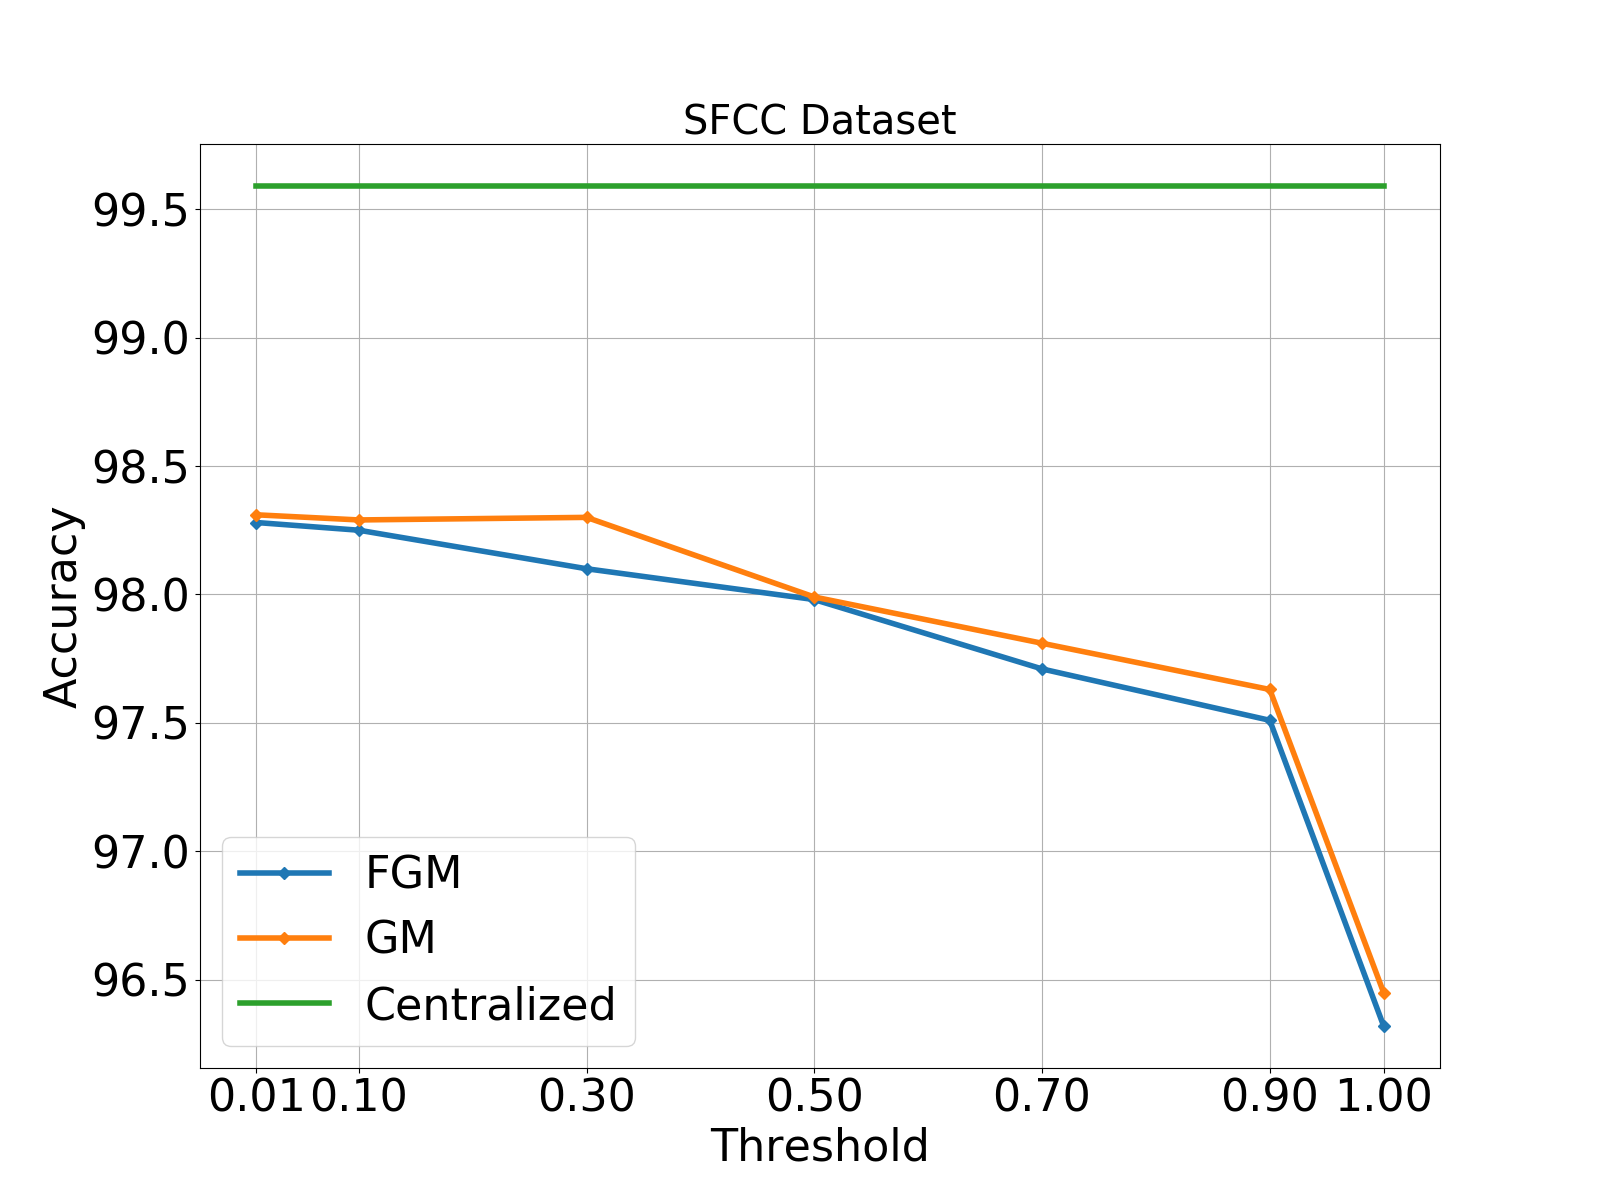
\includegraphics[width=3.9cm,height=3.5cm]{./images/results/sfc-plots/exp_Fig_1_1.png}}
        \subfigure{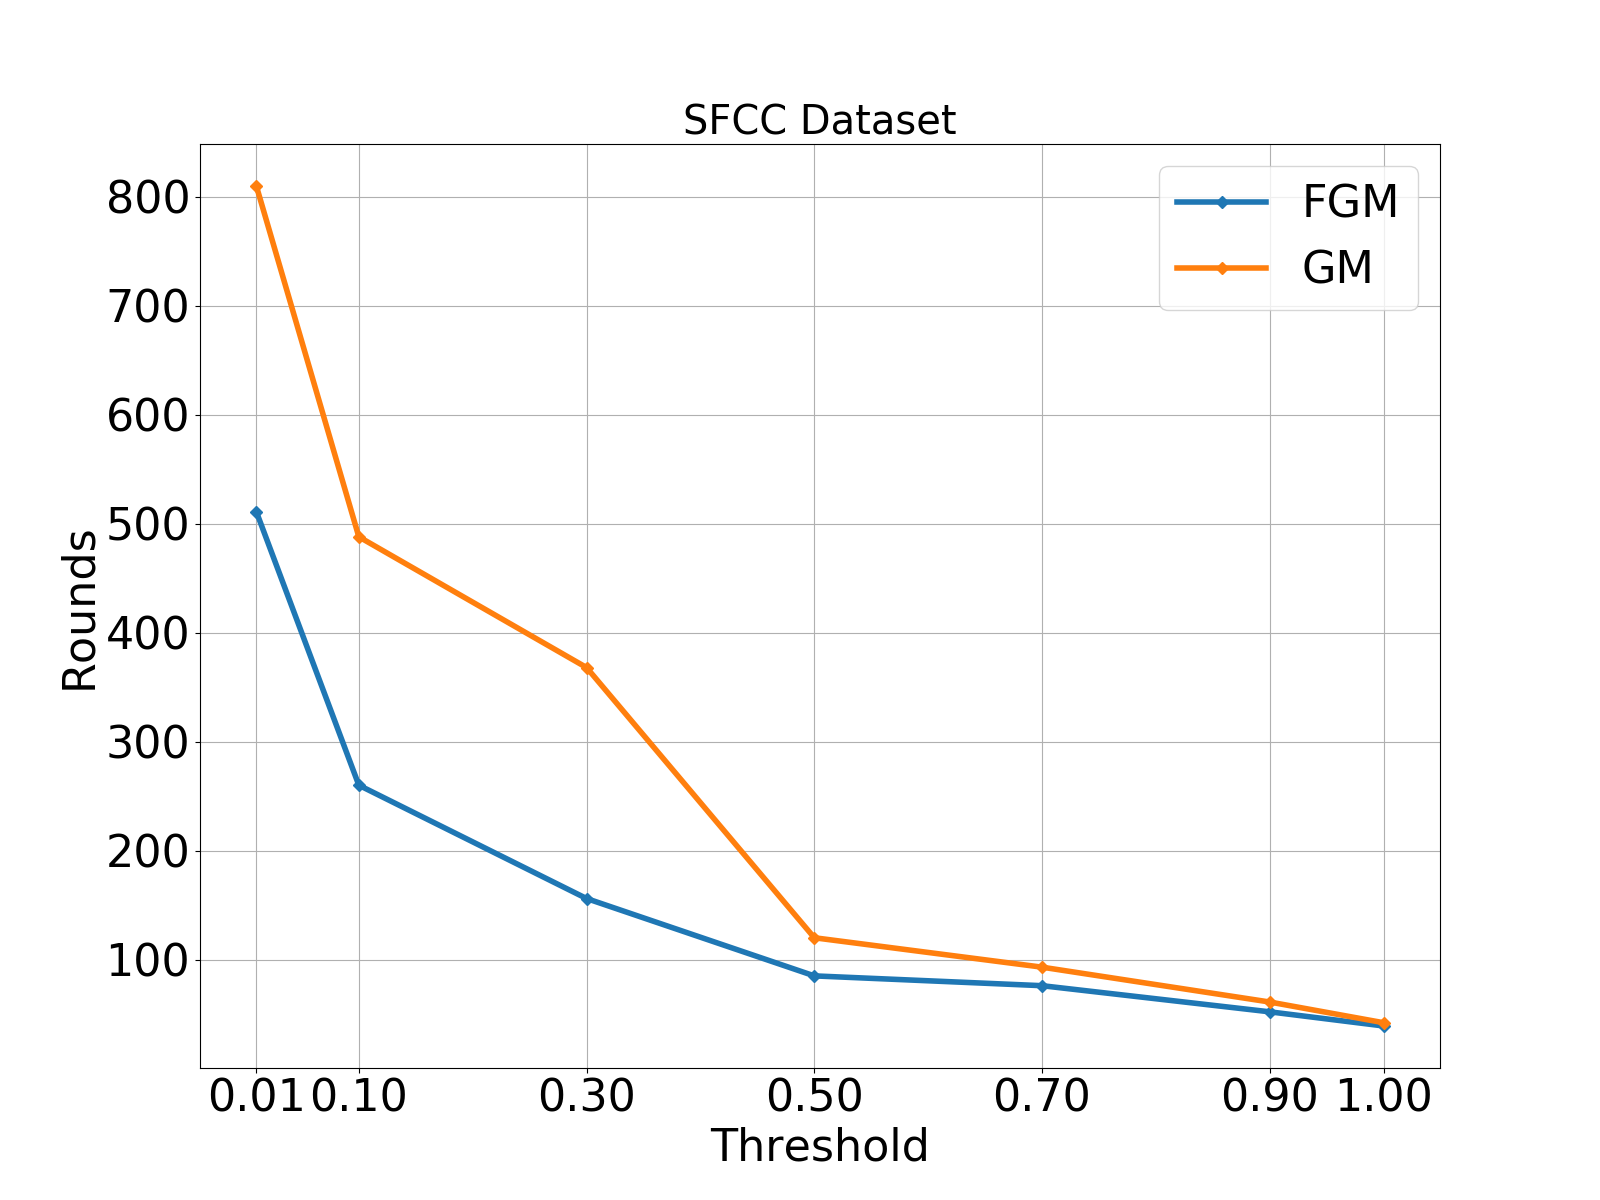
\includegraphics[width=3.9cm,height=3.5cm]{./images/results/sfc-plots/exp_Fig_1_2.png}}
        \subfigure{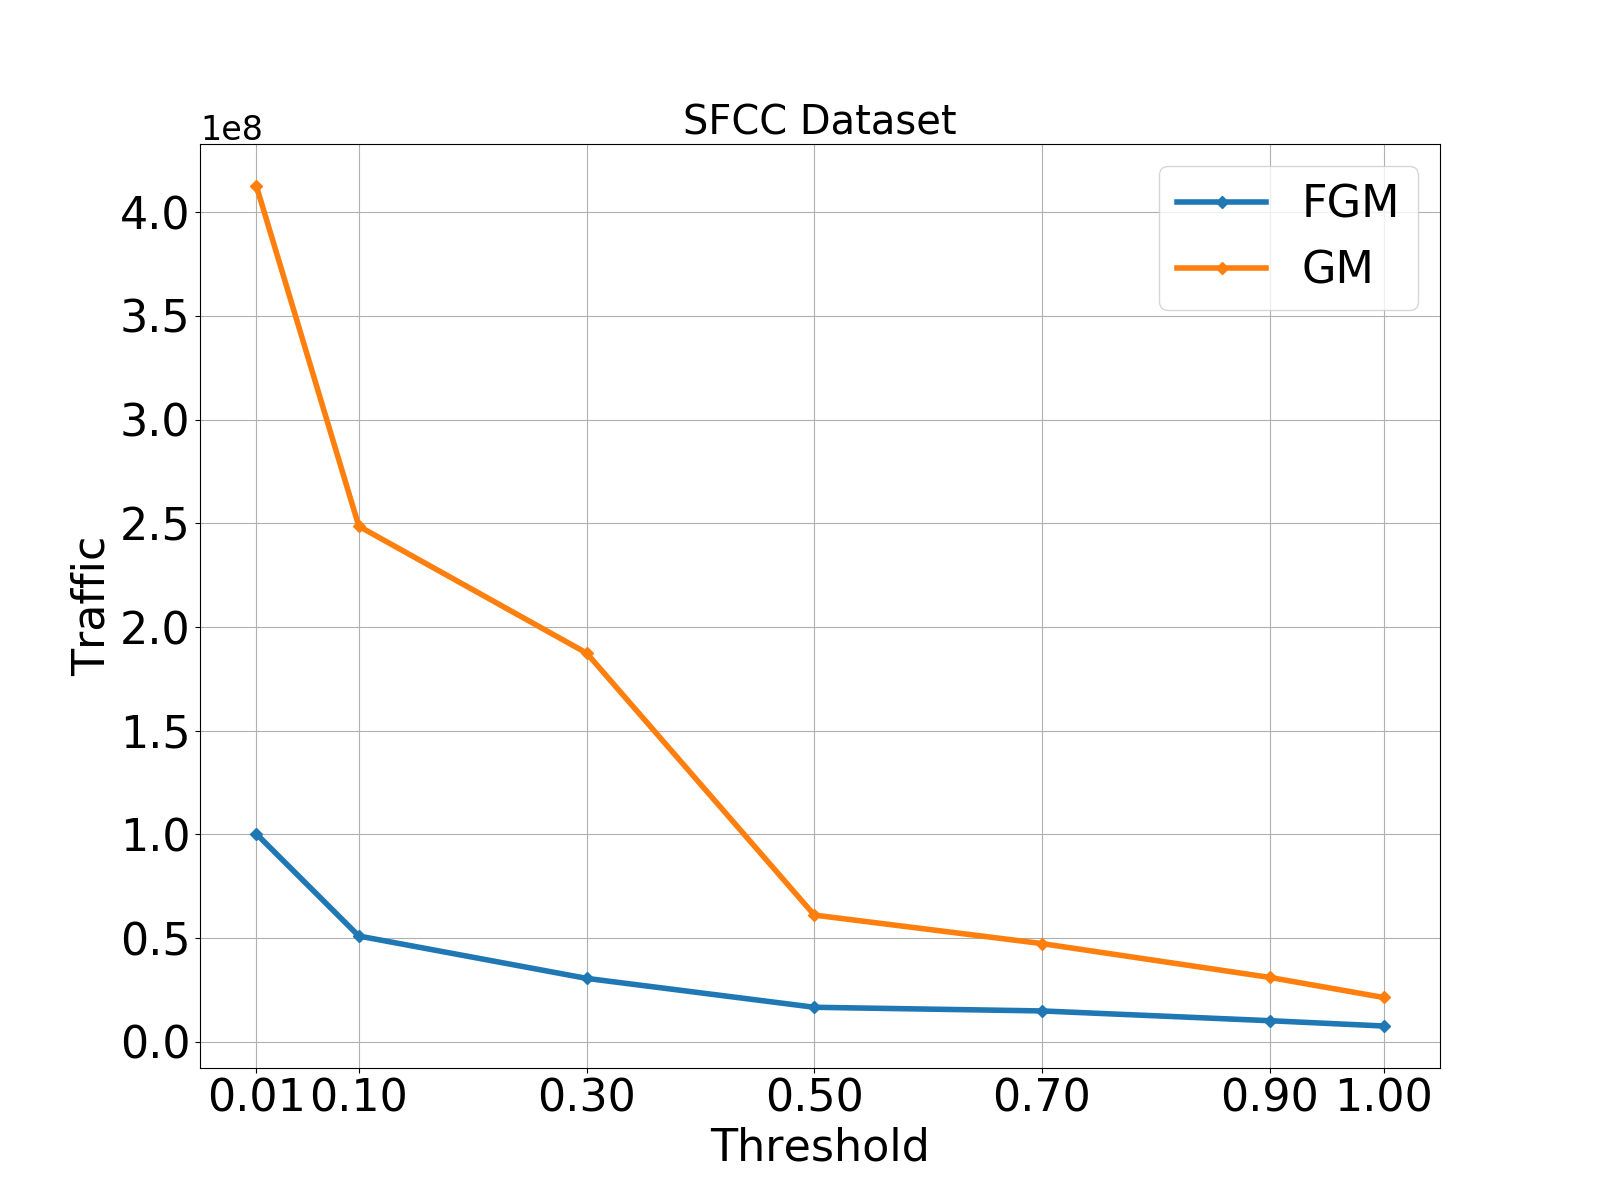
\includegraphics[width=3.9cm,height=3.5cm]{./images/results/sfc-plots/exp_Fig_1_3.png}}
        \subfigure{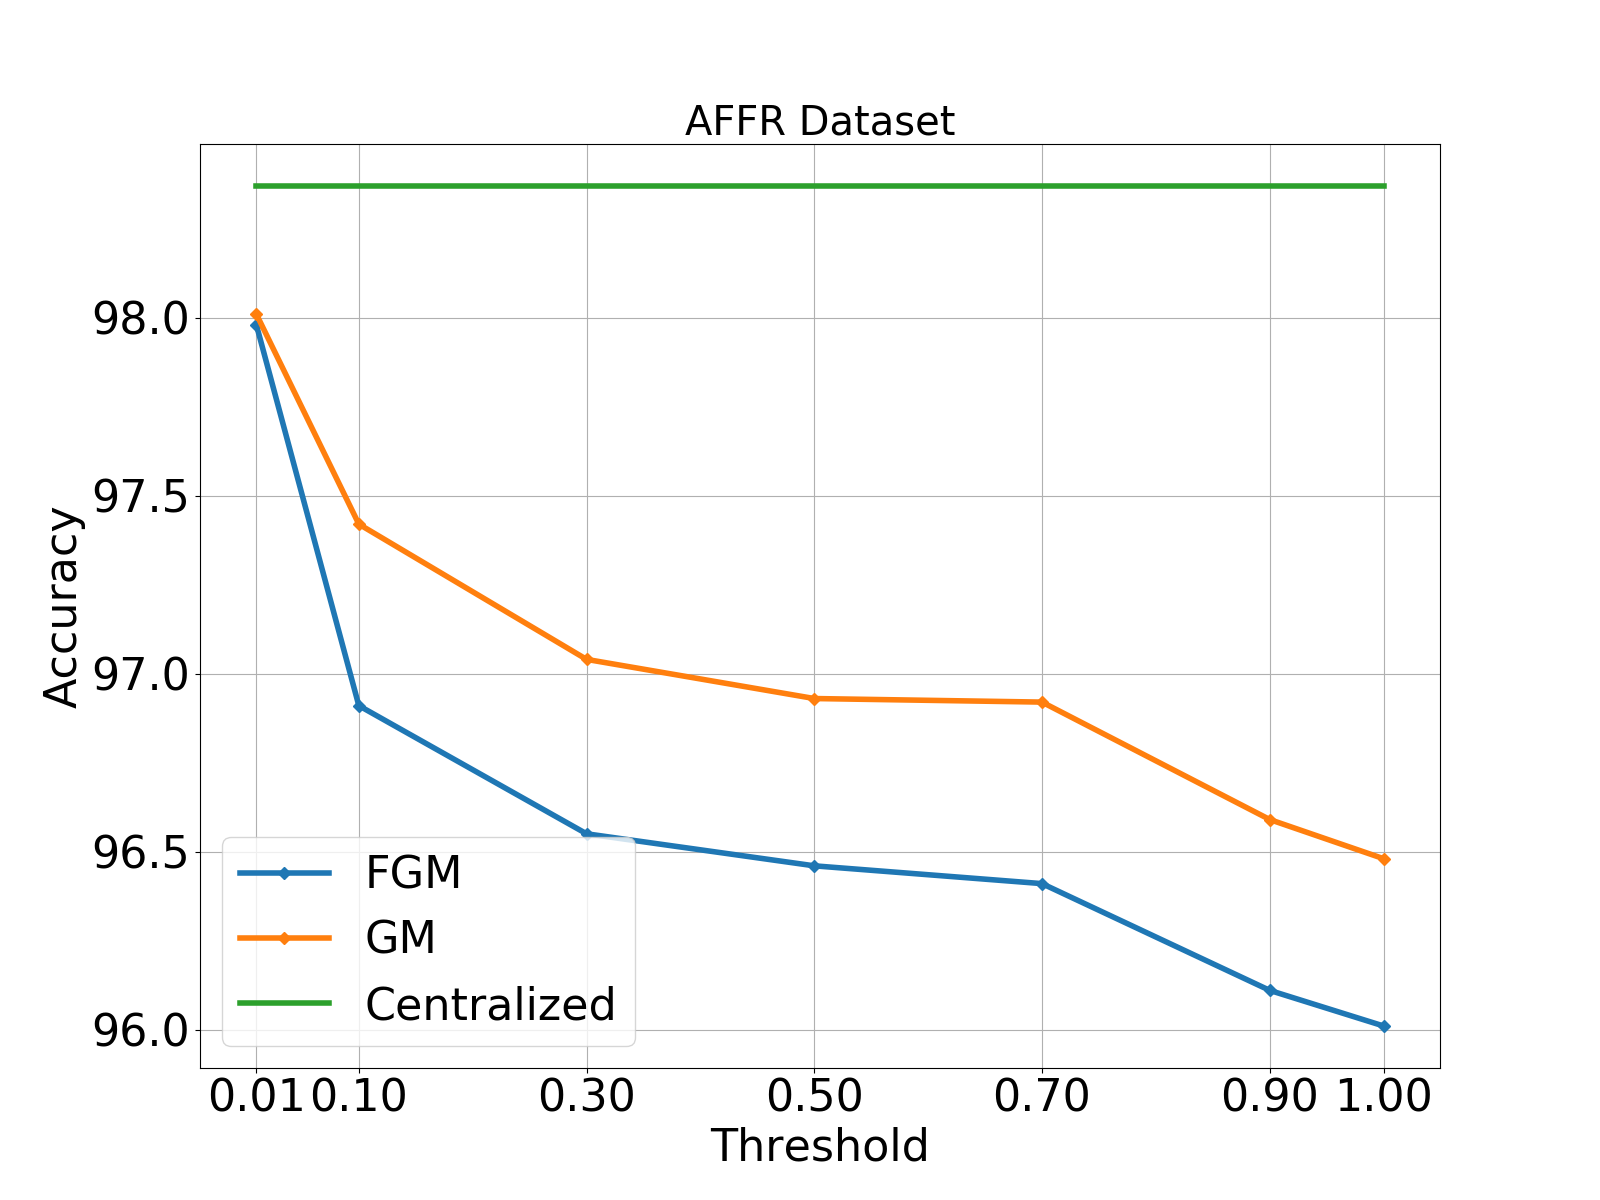
\includegraphics[width=3.9cm,height=3.5cm]{./images/results/amazon-plots/exp_Fig_1_1.png}}
        \subfigure{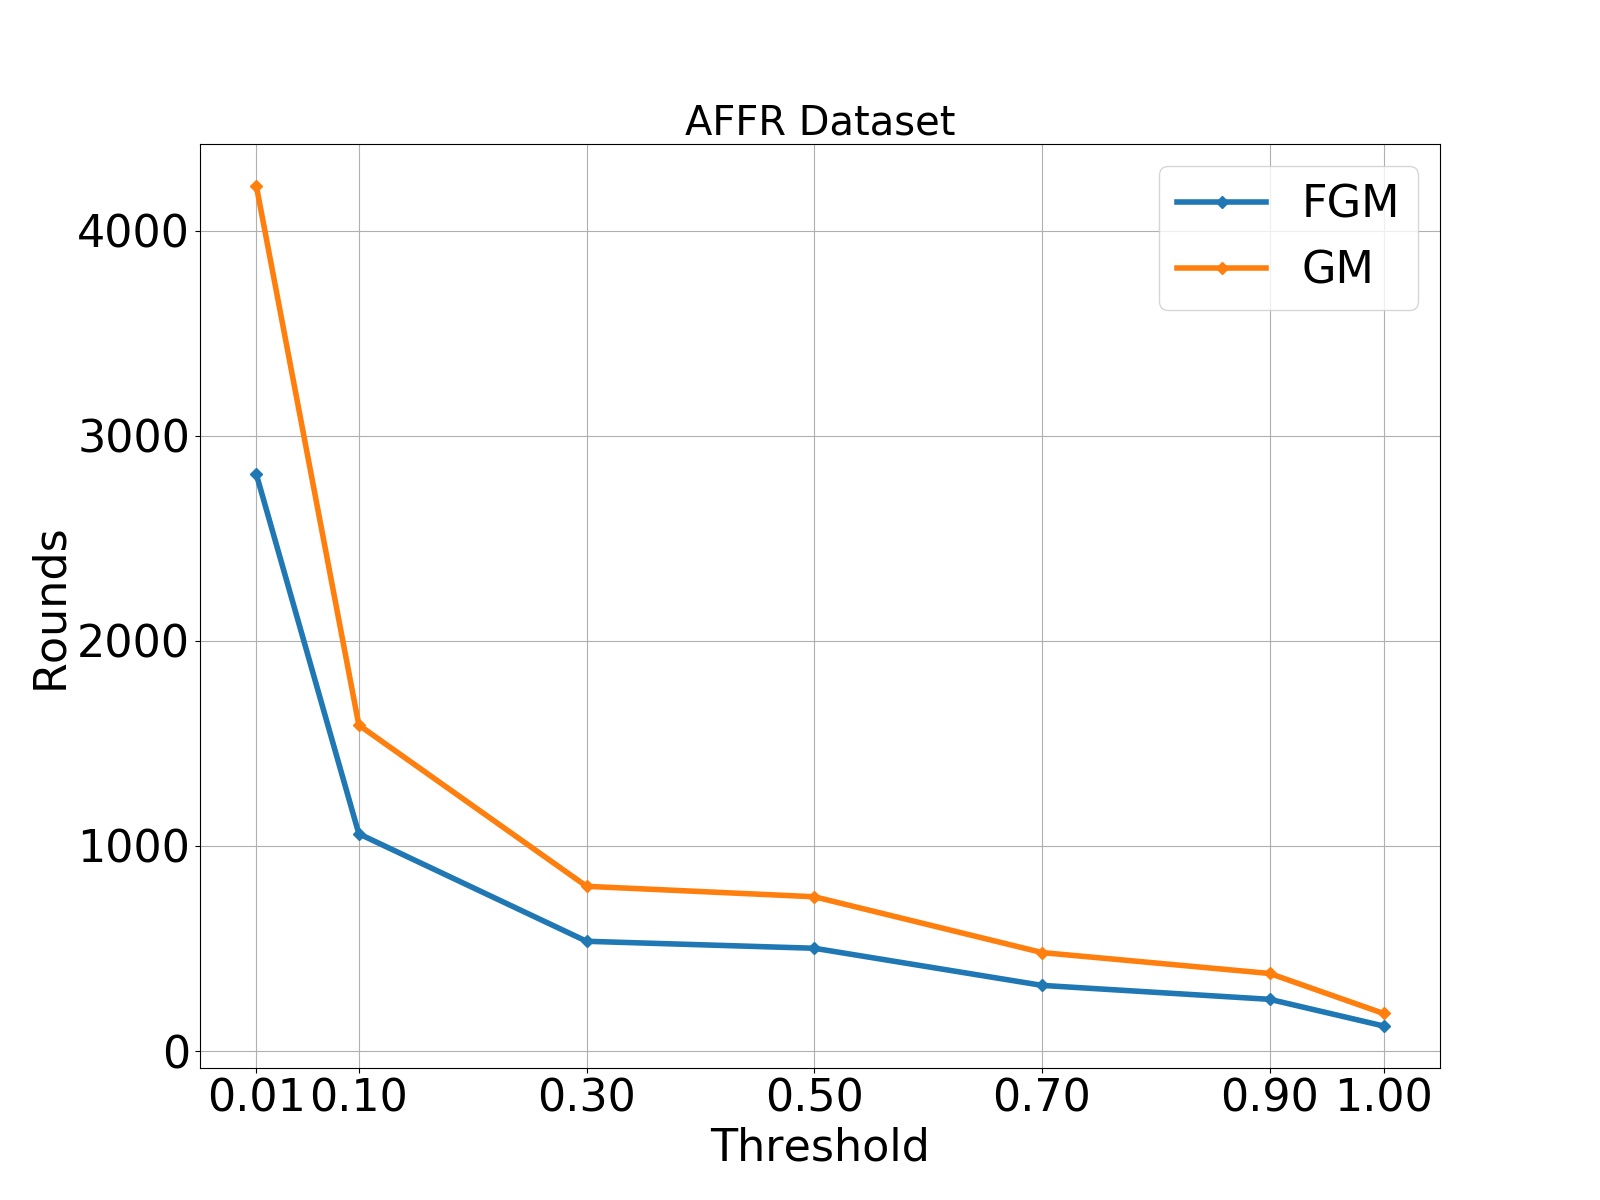
\includegraphics[width=3.9cm,height=3.5cm]{./images/results/amazon-plots/exp_Fig_1_2.png}}
        \subfigure{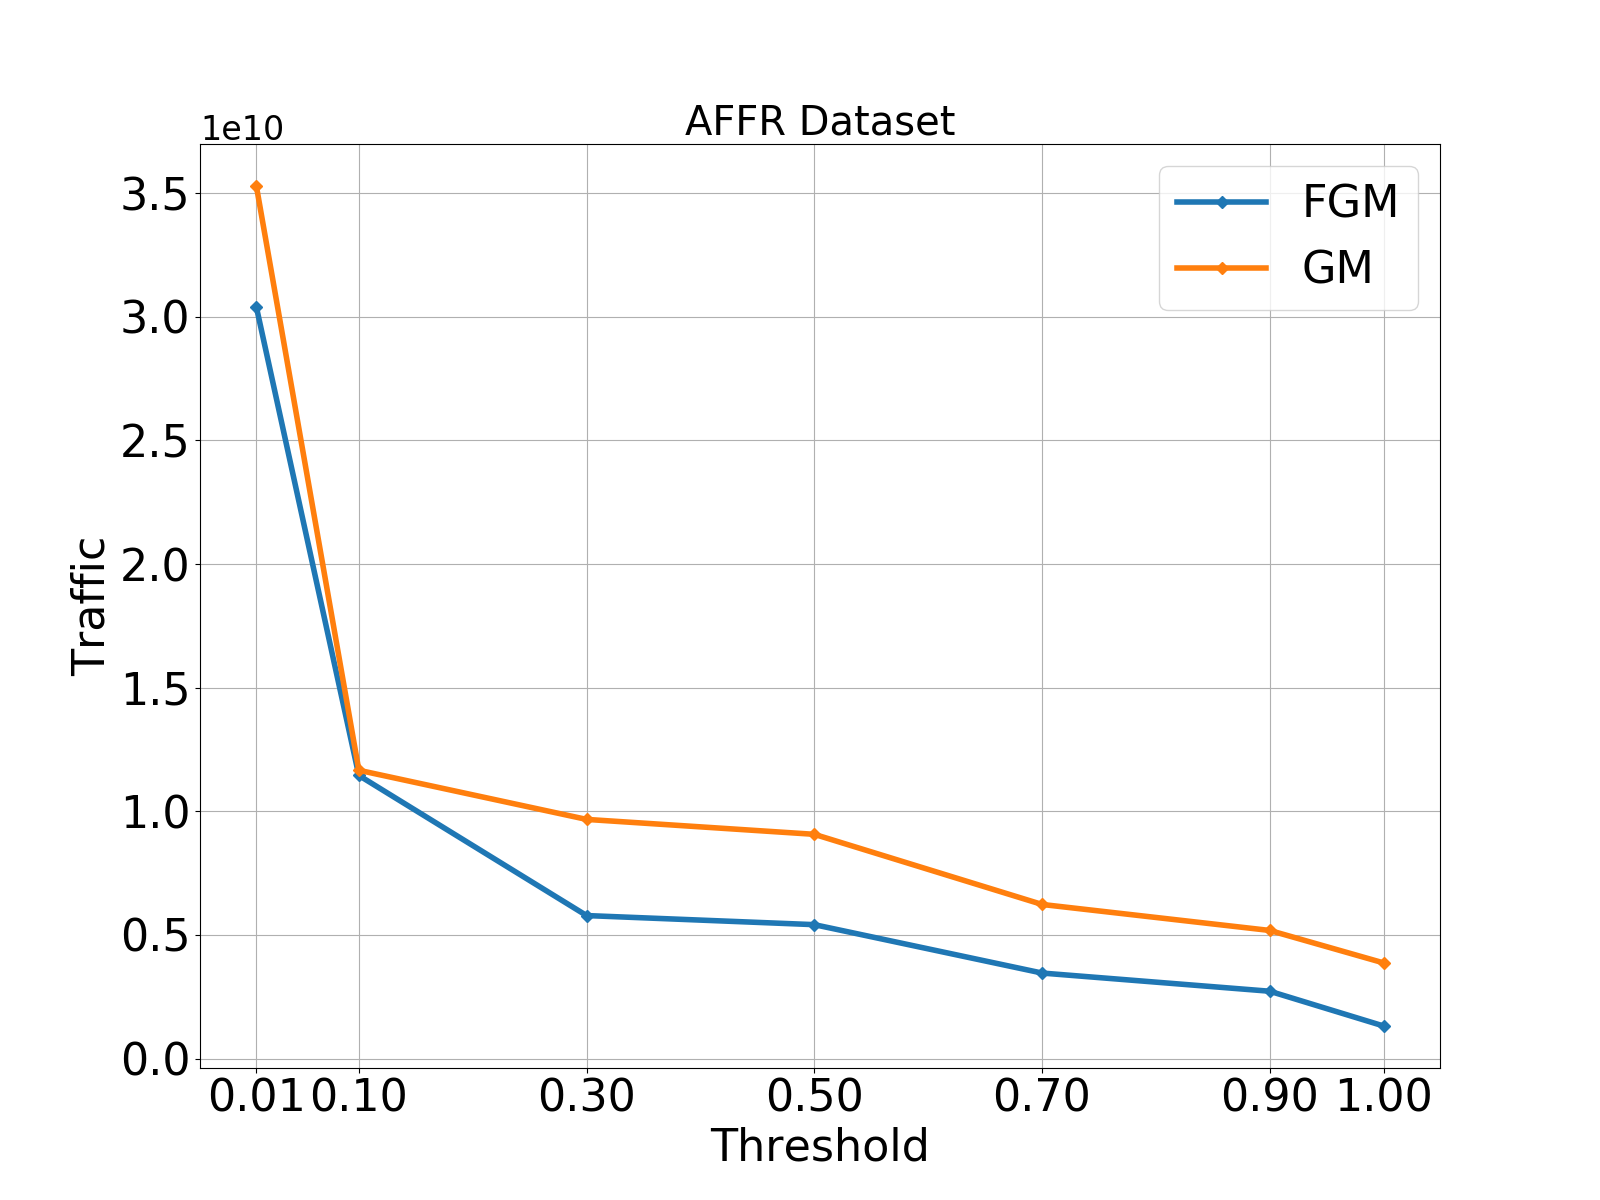
\includegraphics[width=3.9cm,height=3.5cm]{./images/results/amazon-plots/exp_Fig_1_3.png}}
        \label{fig:sfc-amazon-thres}
    \end{figure}
\end{frame}

\begin{frame}{Results (2) - Changing the mini-batch size ($\pmb{|\beta|}$)}
%    \begin{itemize}
%        \item[]{A comment.}
%    \end{itemize}
%    \vspace{-0.4cm}
    \begin{figure}
        \subfigure{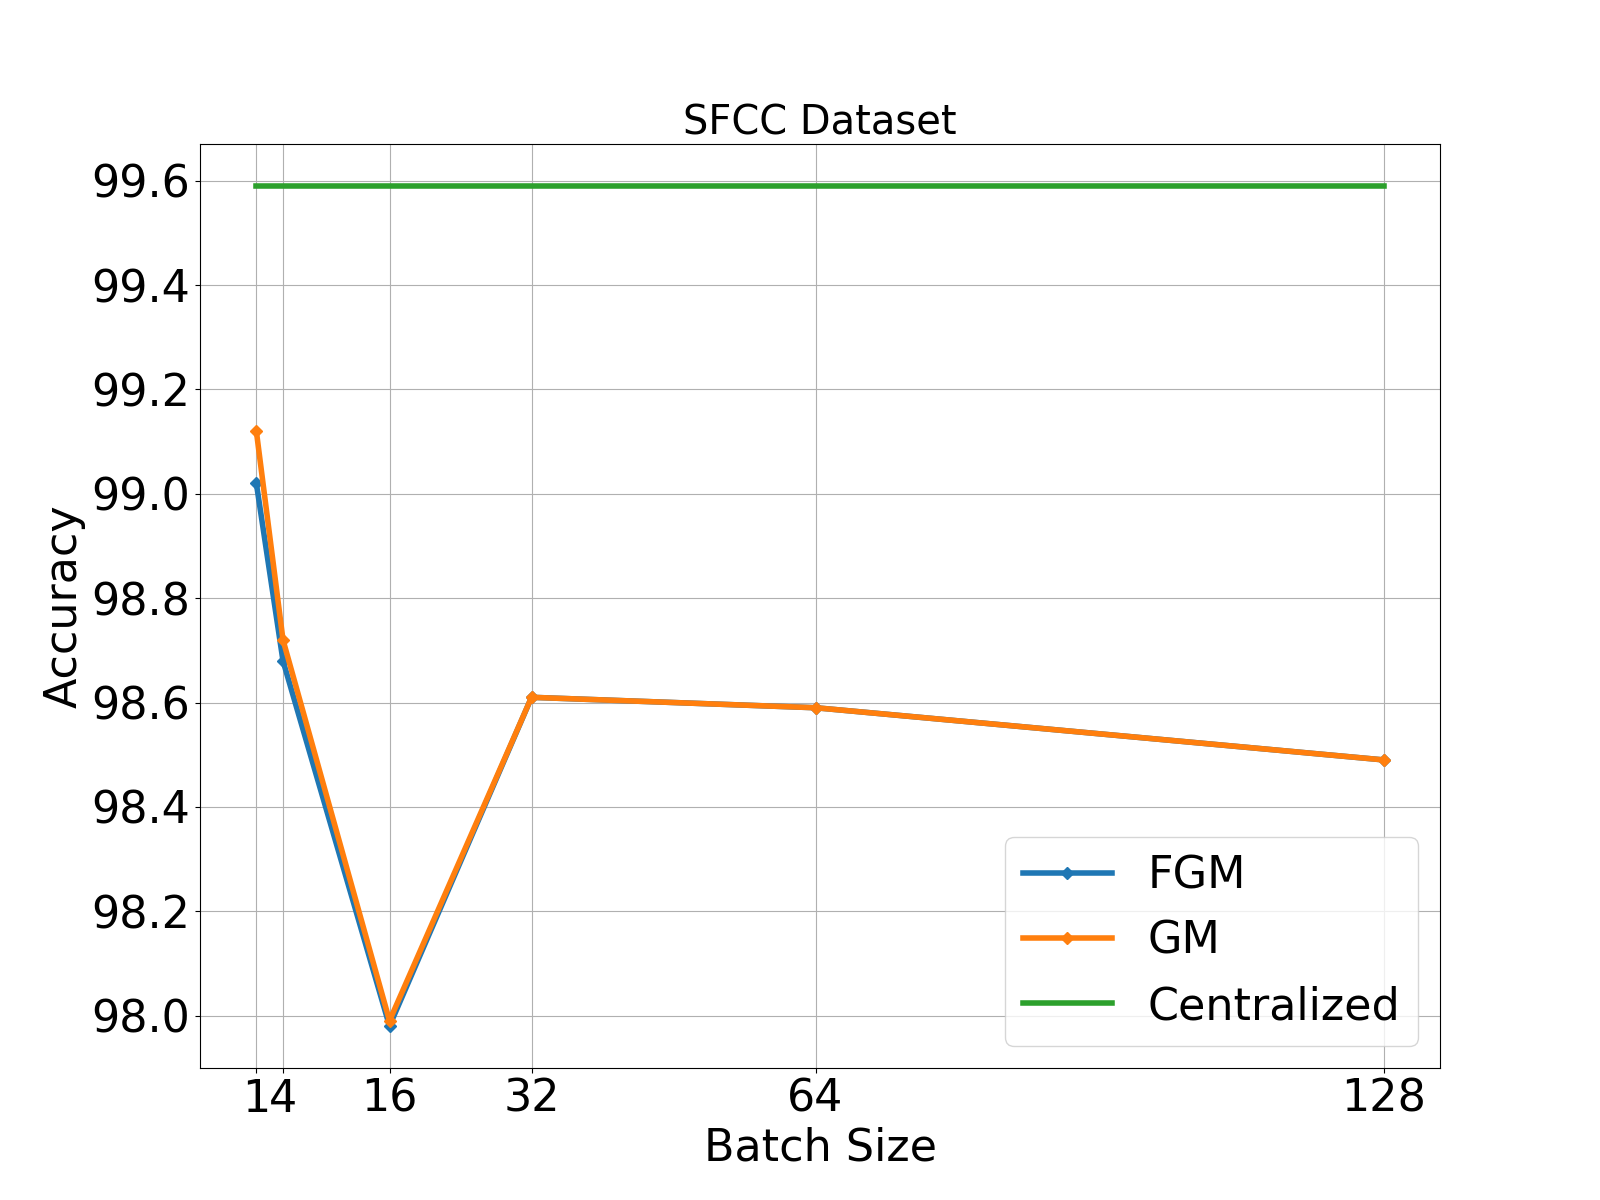
\includegraphics[width=3.9cm,height=3.5cm]{./images/results/sfc-plots/exp_Fig_2_1.png}}
        \subfigure{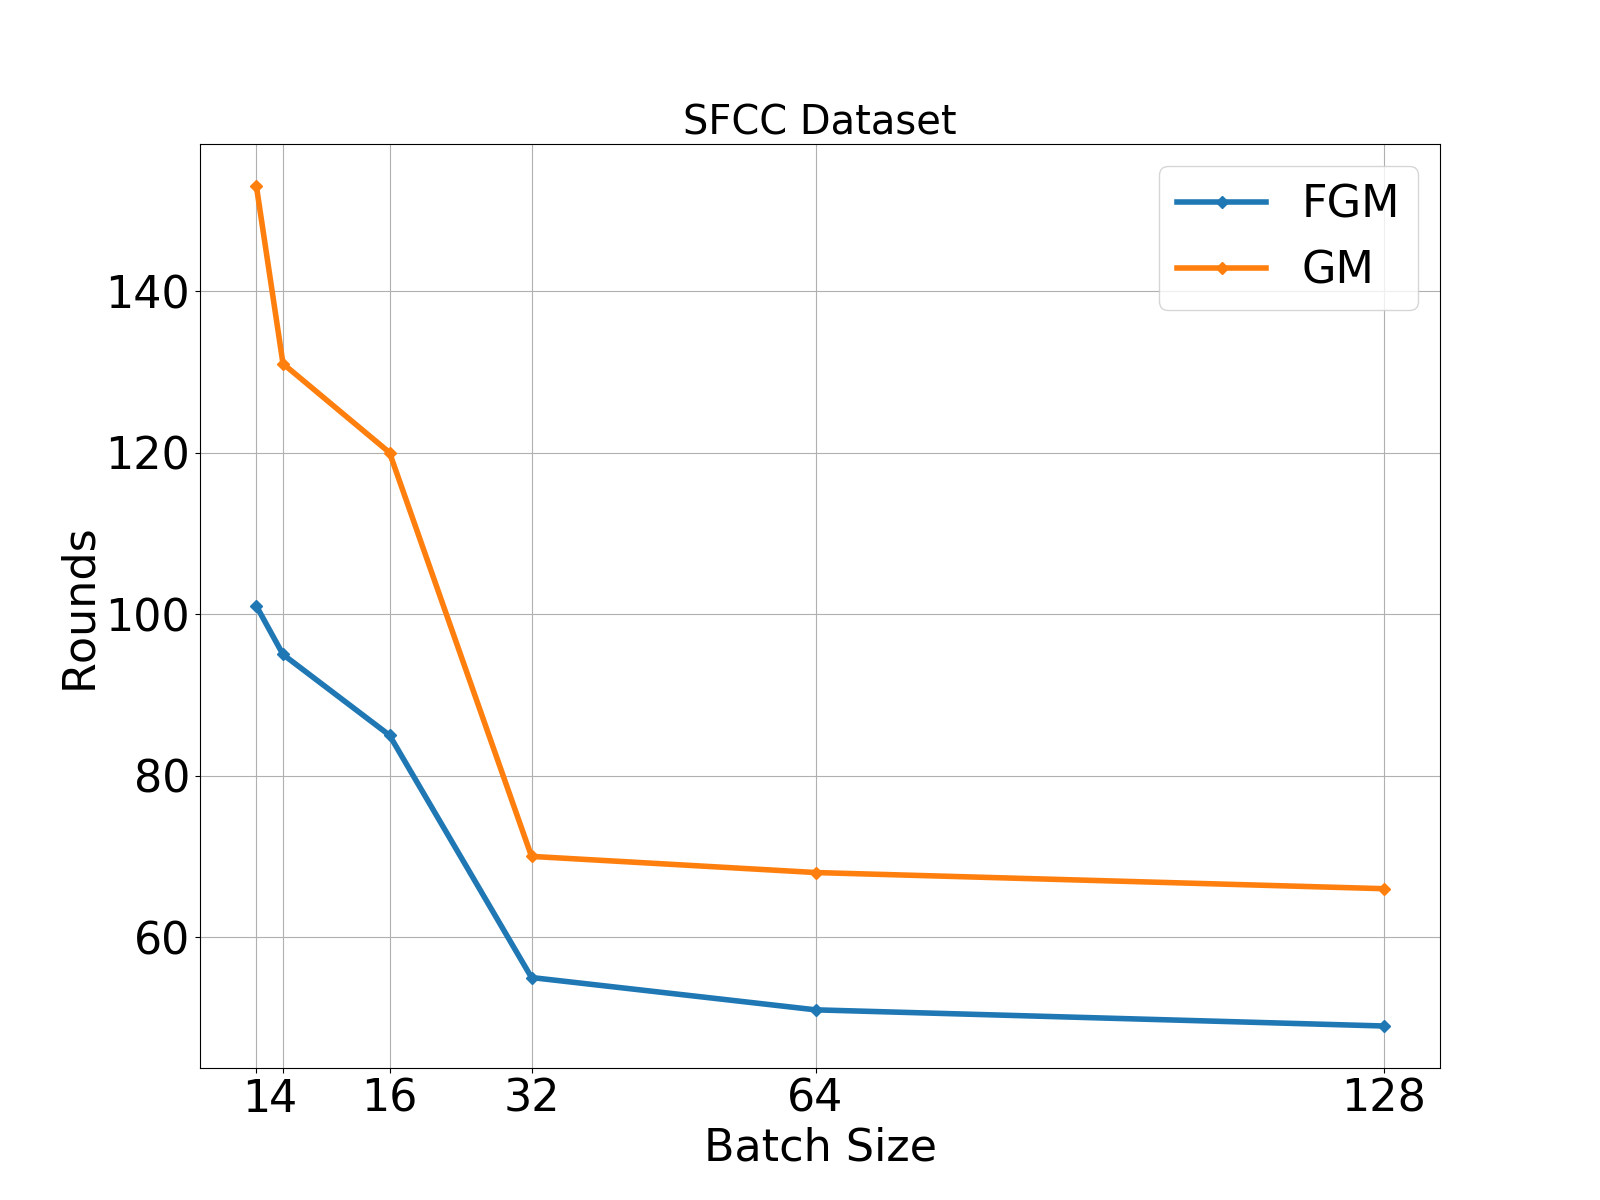
\includegraphics[width=3.9cm,height=3.5cm]{./images/results/sfc-plots/exp_Fig_2_2.png}}
        \subfigure{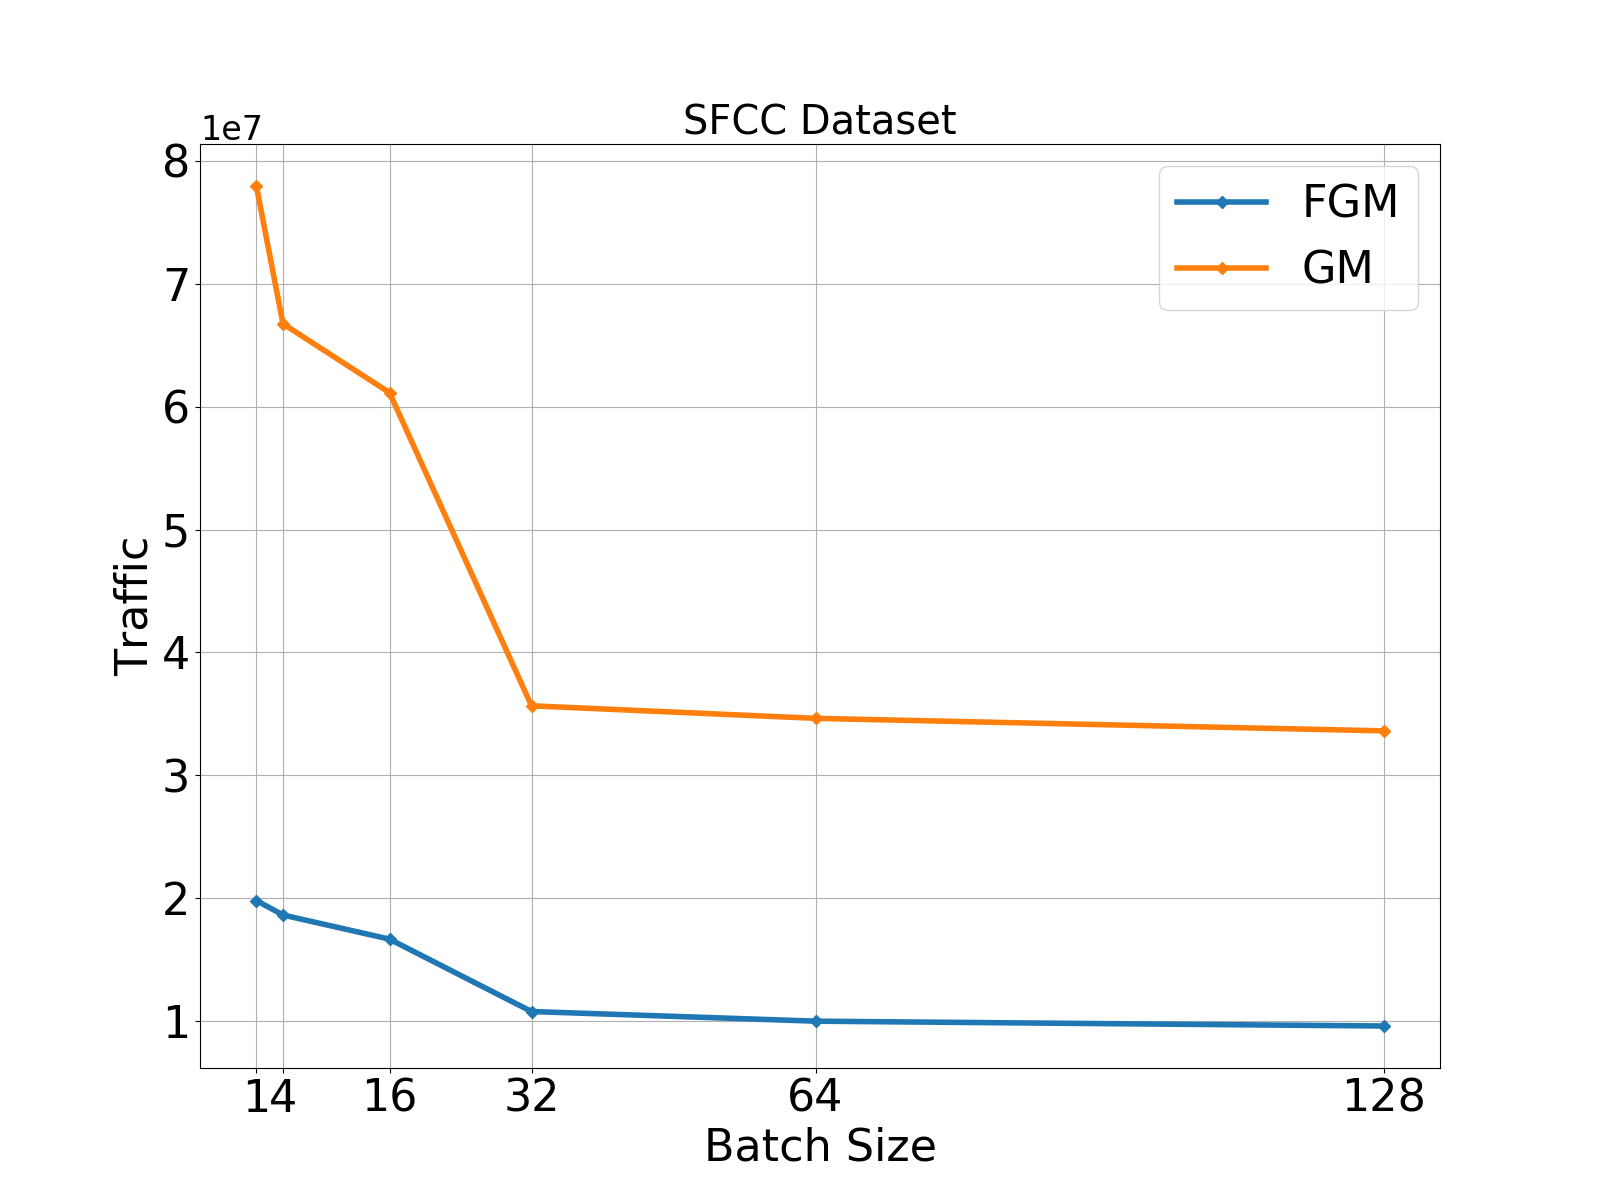
\includegraphics[width=3.9cm,height=3.5cm]{./images/results/sfc-plots/exp_Fig_2_3.png}}
        \subfigure{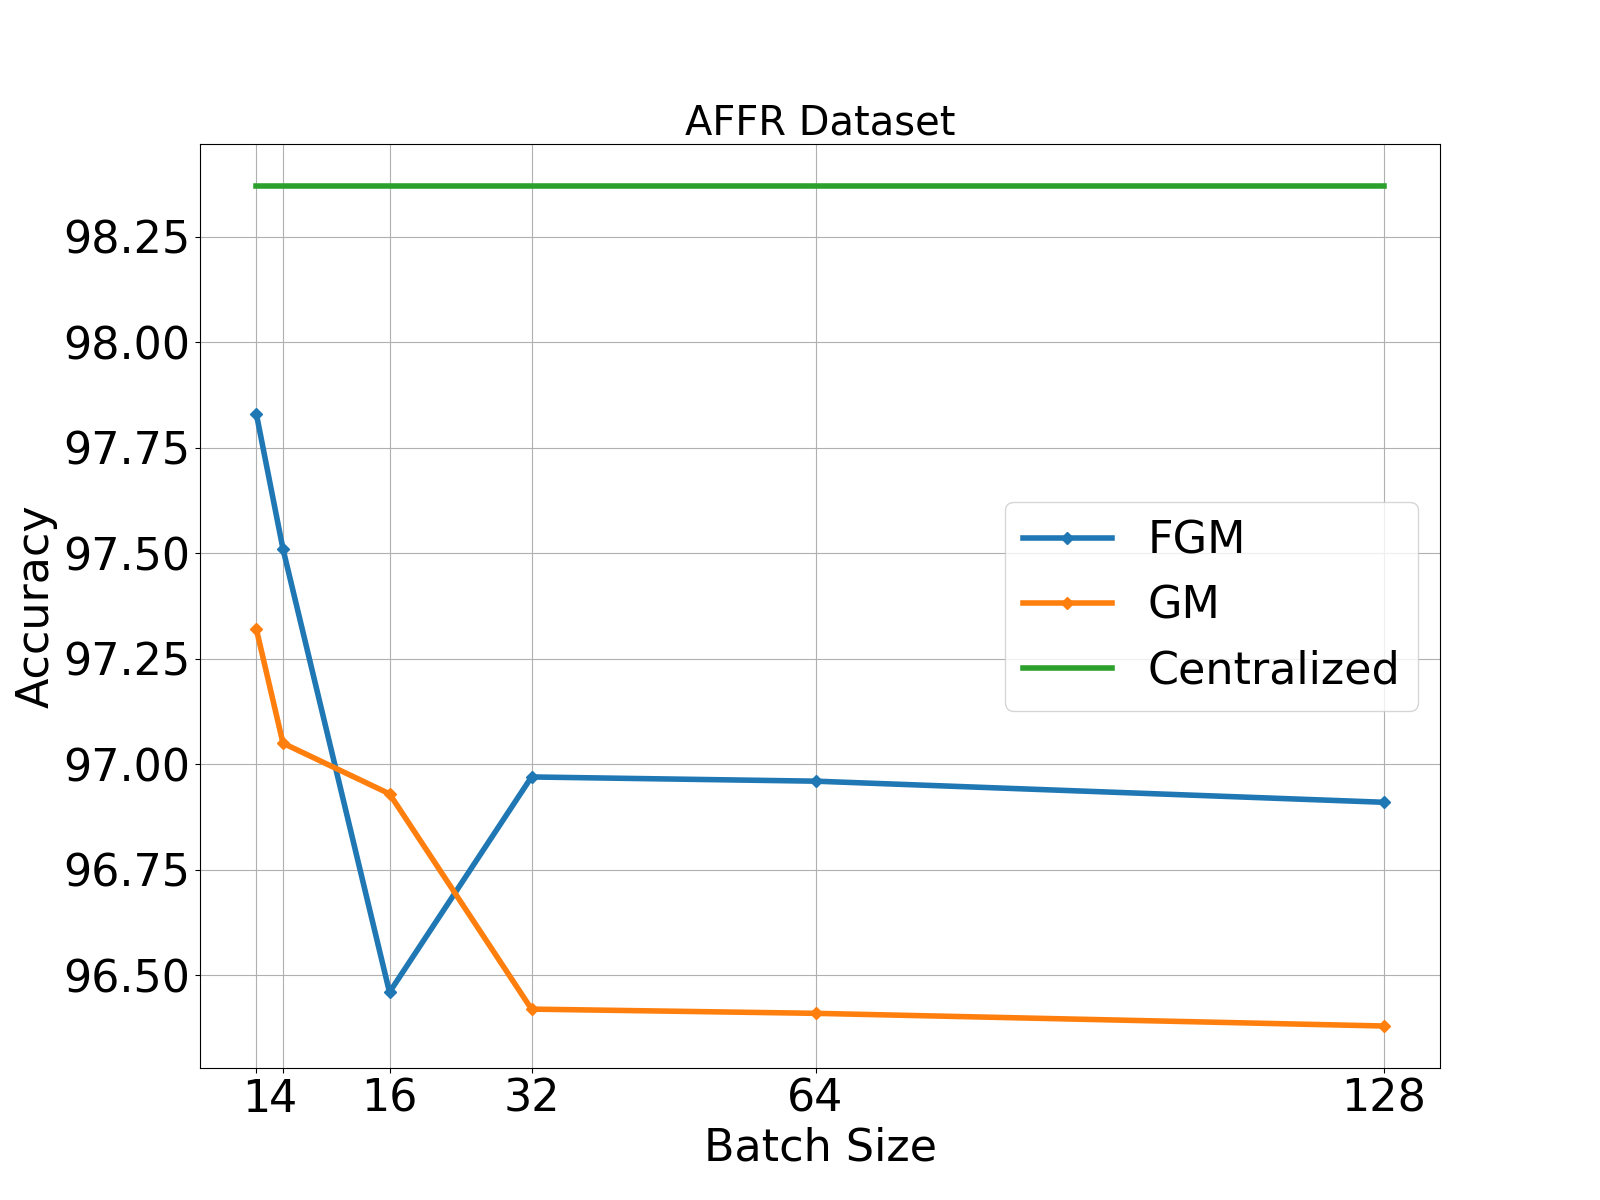
\includegraphics[width=3.9cm,height=3.5cm]{./images/results/amazon-plots/exp_Fig_2_1.png}}
        \subfigure{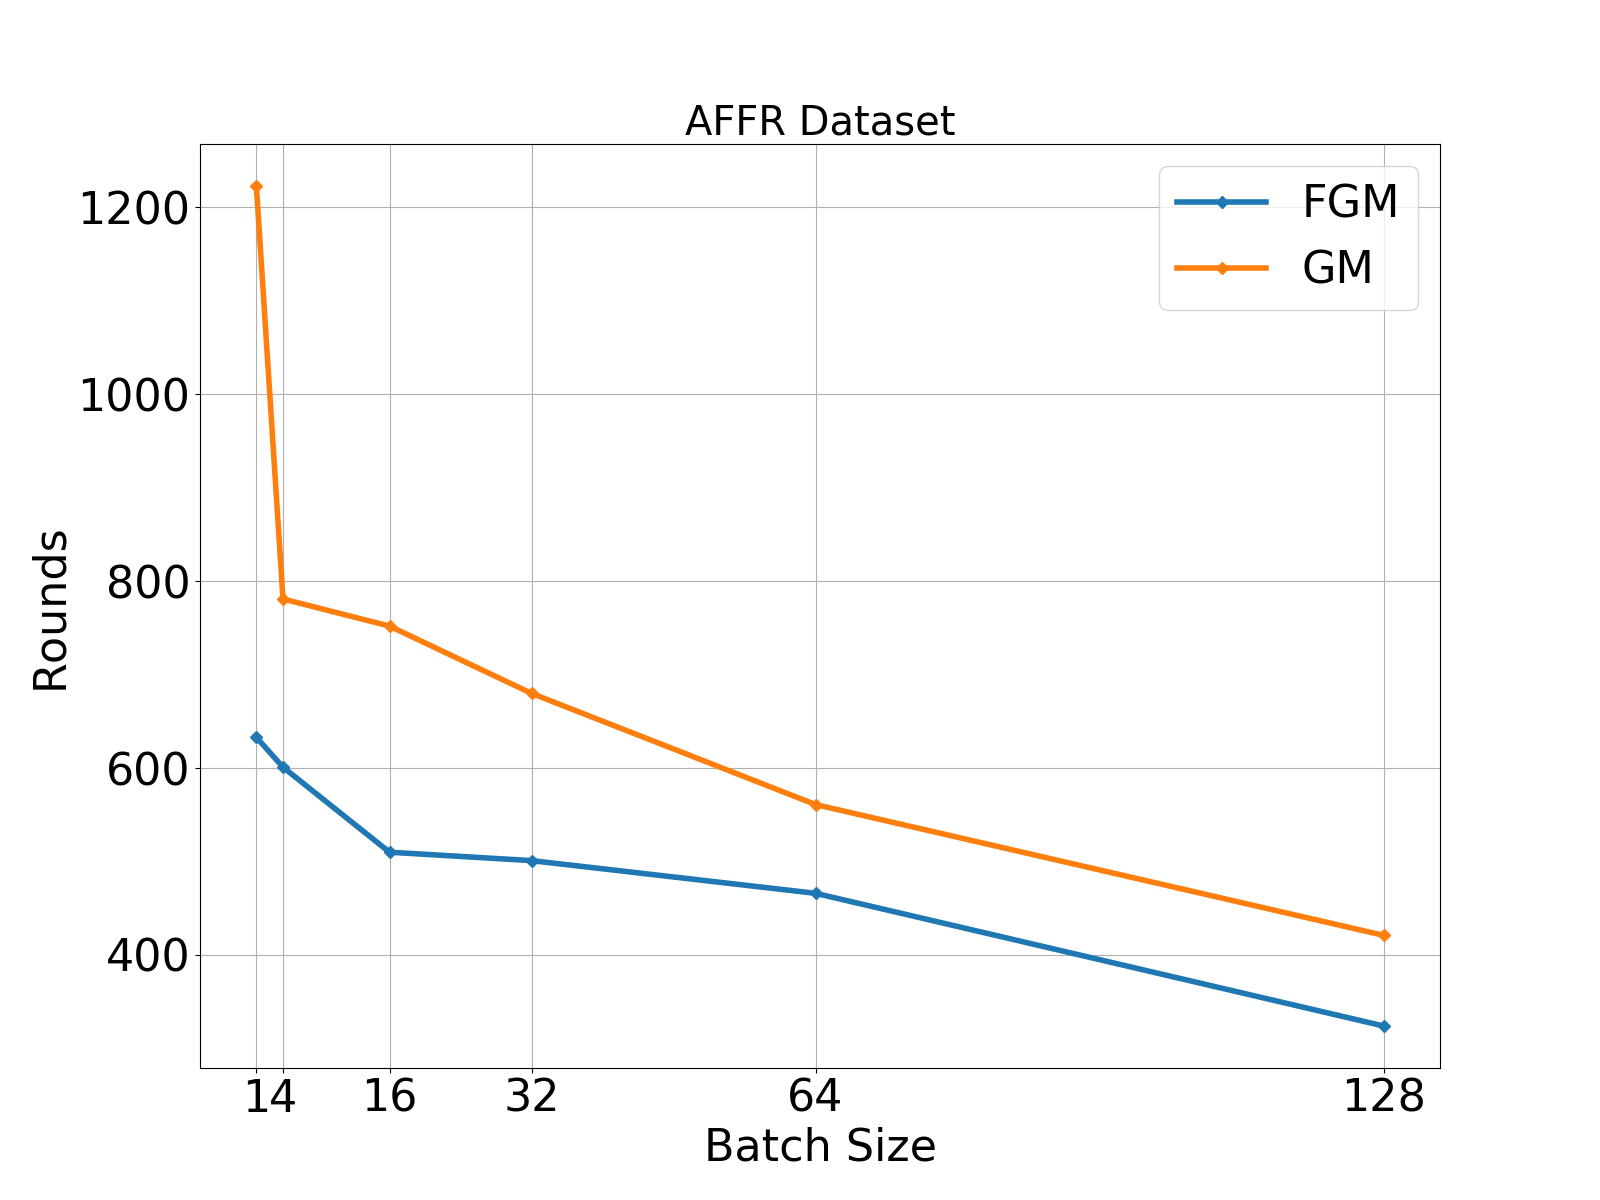
\includegraphics[width=3.9cm,height=3.5cm]{./images/results/amazon-plots/exp_Fig_2_2.png}}
        \subfigure{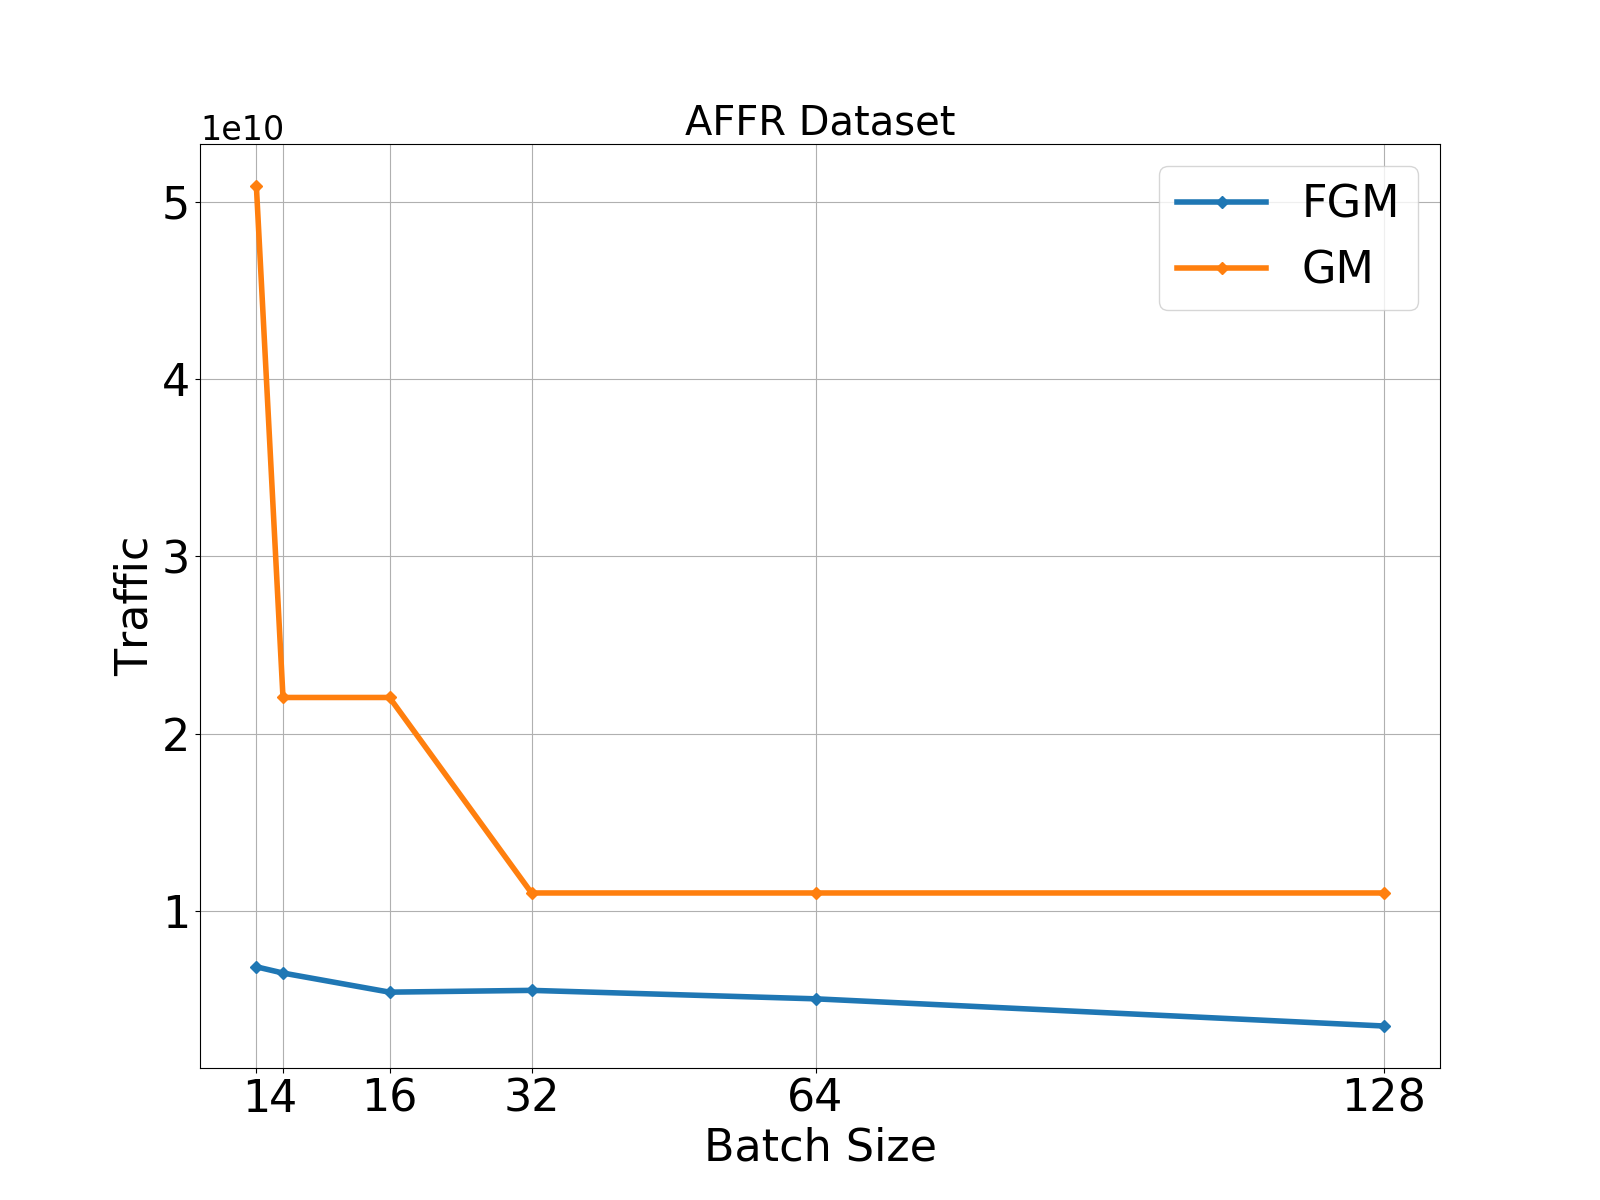
\includegraphics[width=3.9cm,height=3.5cm]{./images/results/amazon-plots/exp_Fig_2_3.png}}
        \label{fig:sfc-amazon-bs}
    \end{figure}
\end{frame}

\begin{frame}{Results (3) - Changing the number of workers ($\pmb{n}$)}
%    \begin{itemize}
%        \item[]{A comment.}
%    \end{itemize}
%    \vspace{-0.4cm}
    \begin{figure}
        \subfigure{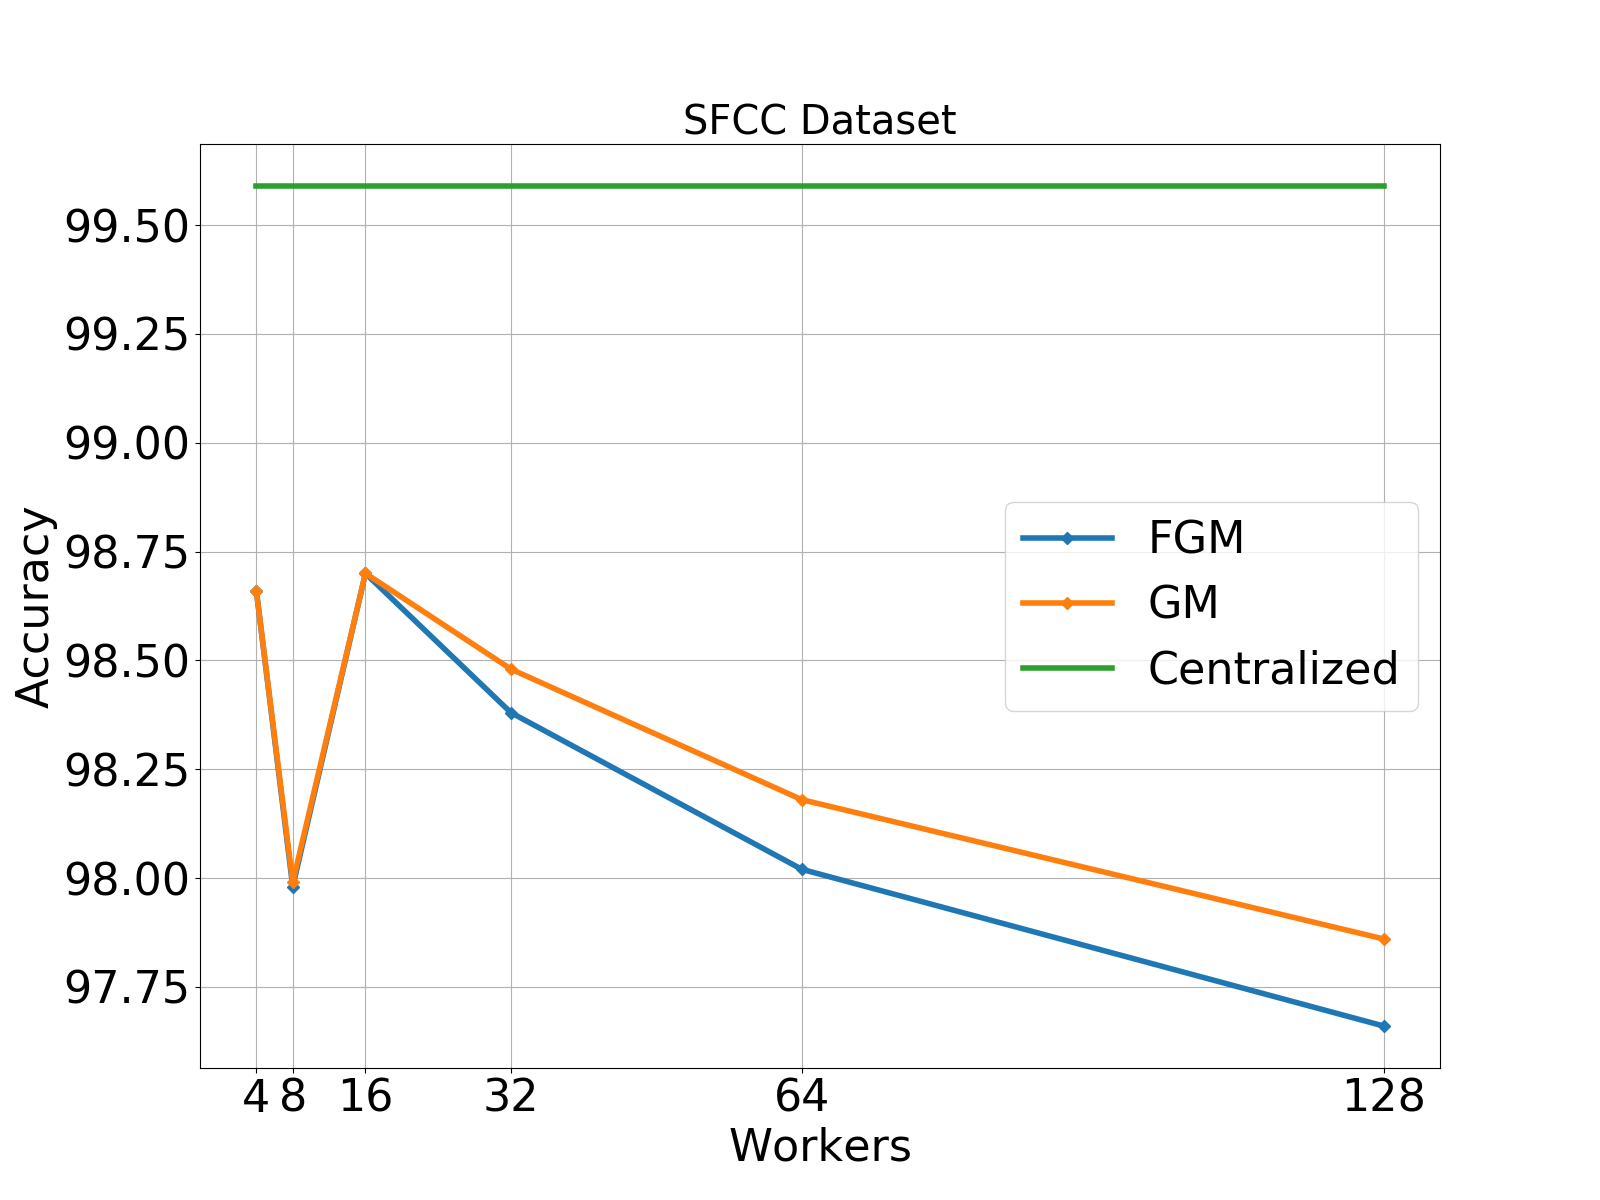
\includegraphics[width=3.9cm,height=3.5cm]{./images/results/sfc-plots/exp_Fig_3_1.png}}
        \subfigure{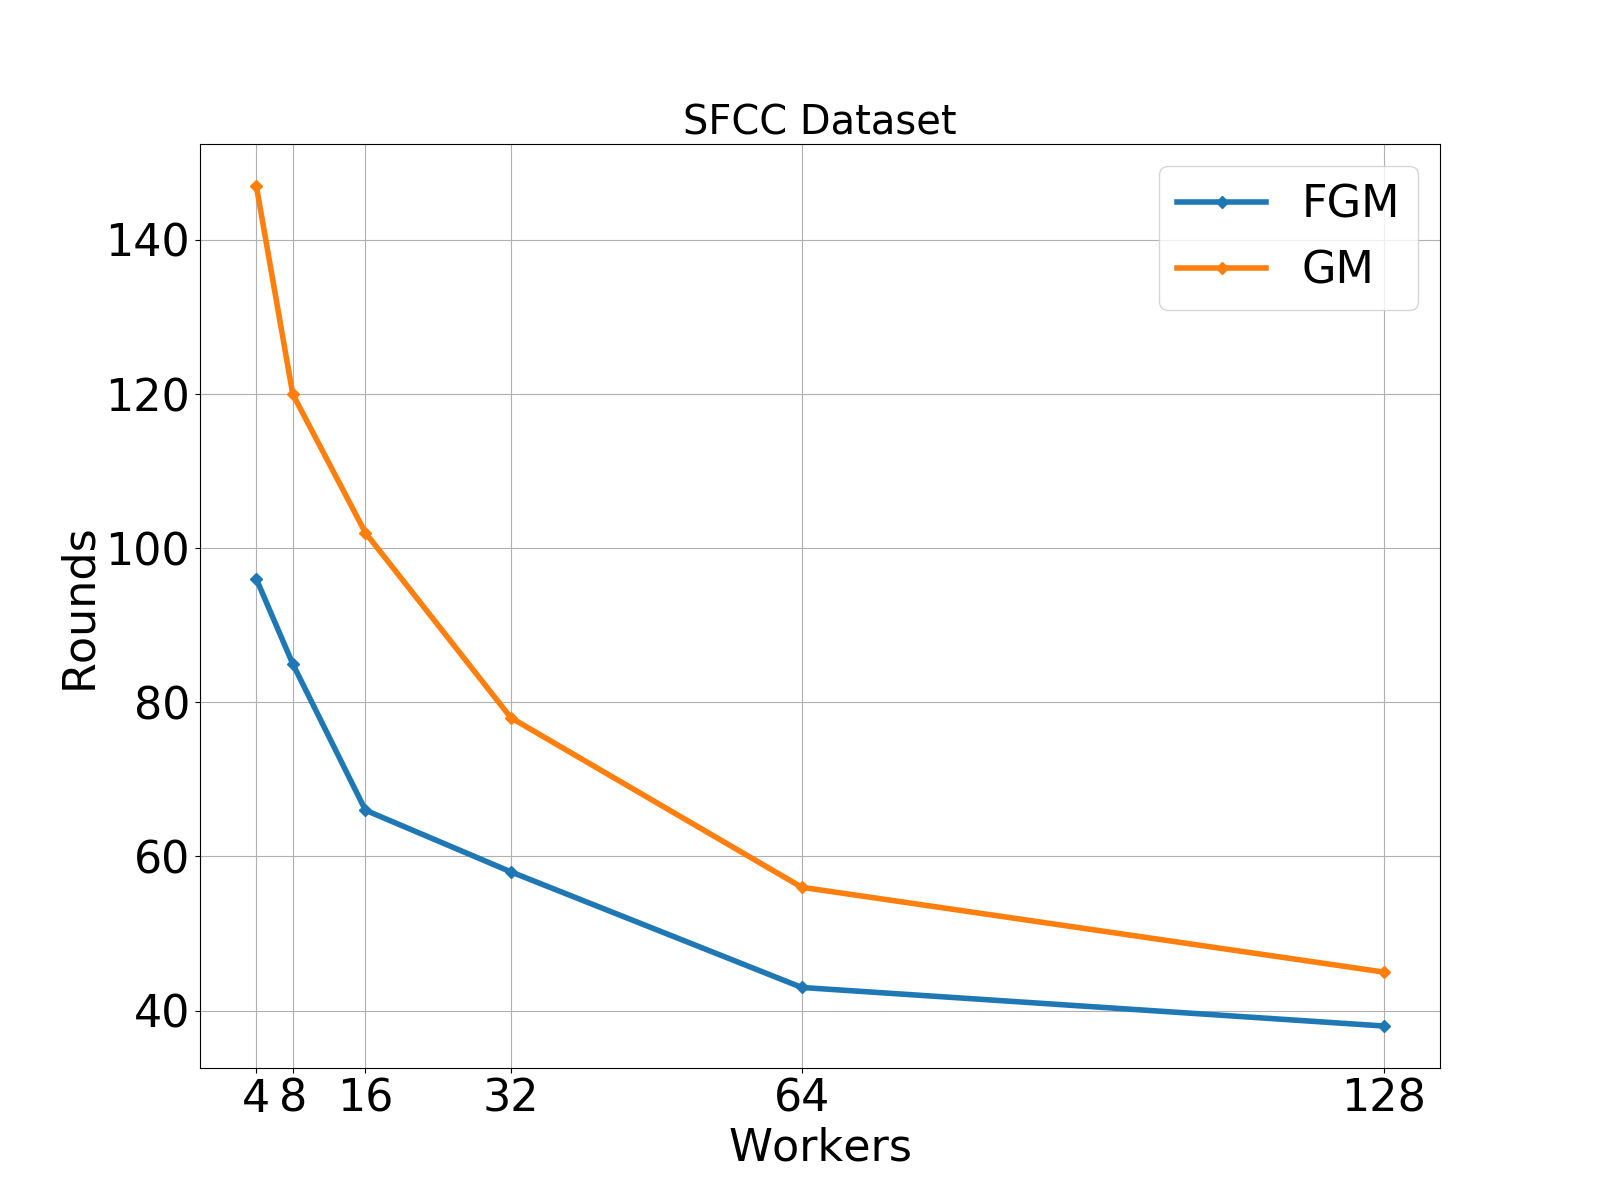
\includegraphics[width=3.9cm,height=3.5cm]{./images/results/sfc-plots/exp_Fig_3_2.png}}
        \subfigure{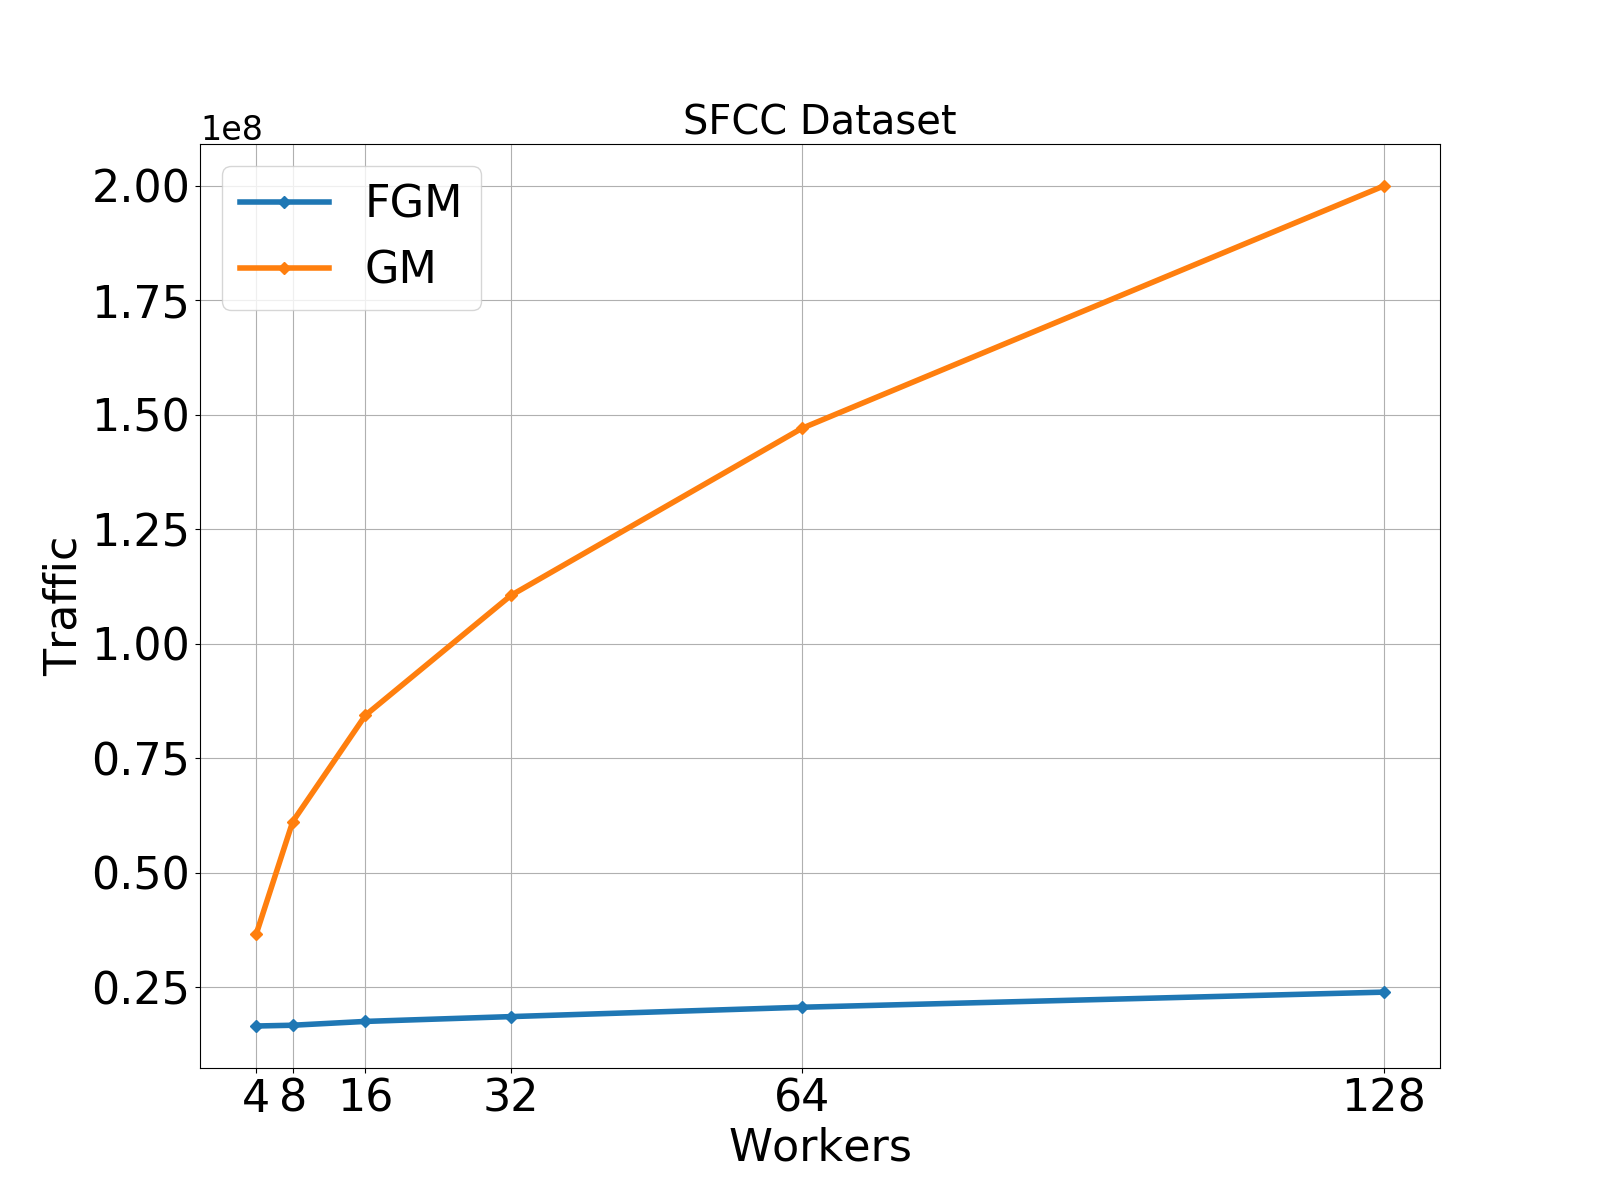
\includegraphics[width=3.9cm,height=3.5cm]{./images/results/sfc-plots/exp_Fig_3_3.png}}
        \subfigure{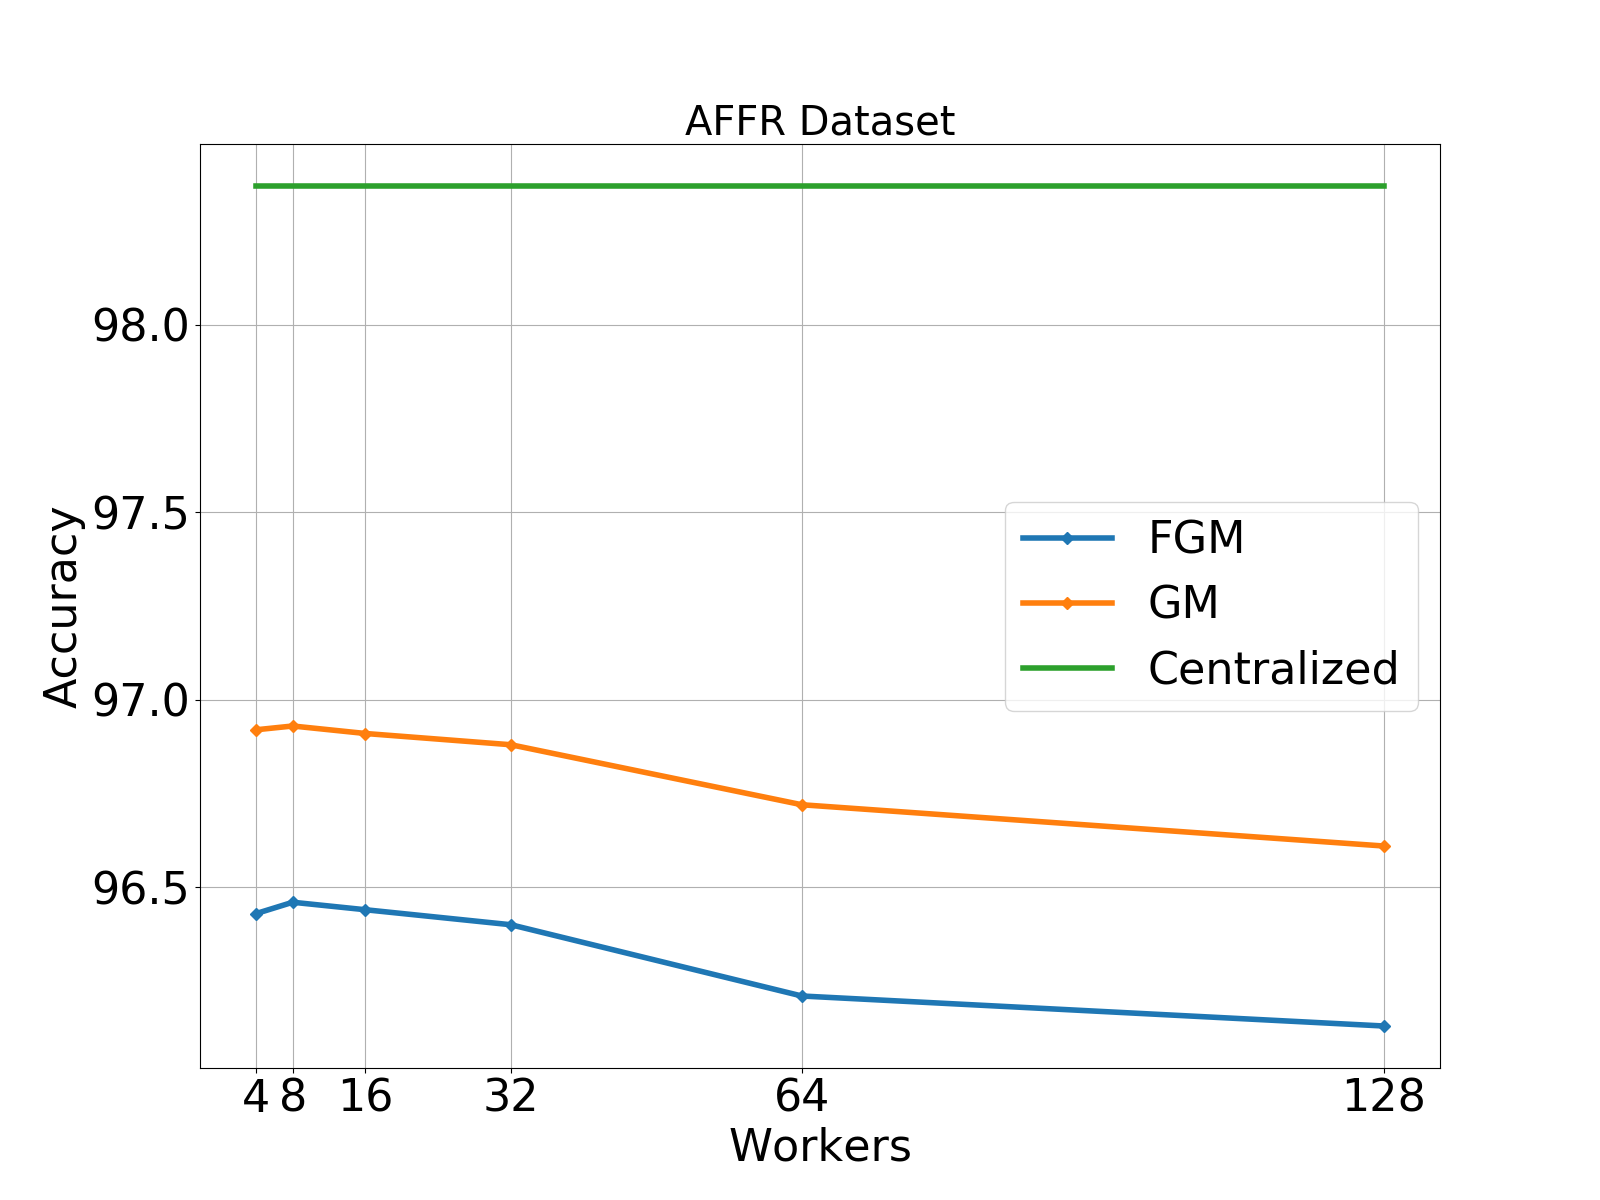
\includegraphics[width=3.9cm,height=3.5cm]{./images/results/amazon-plots/exp_Fig_3_1.png}}
        \subfigure{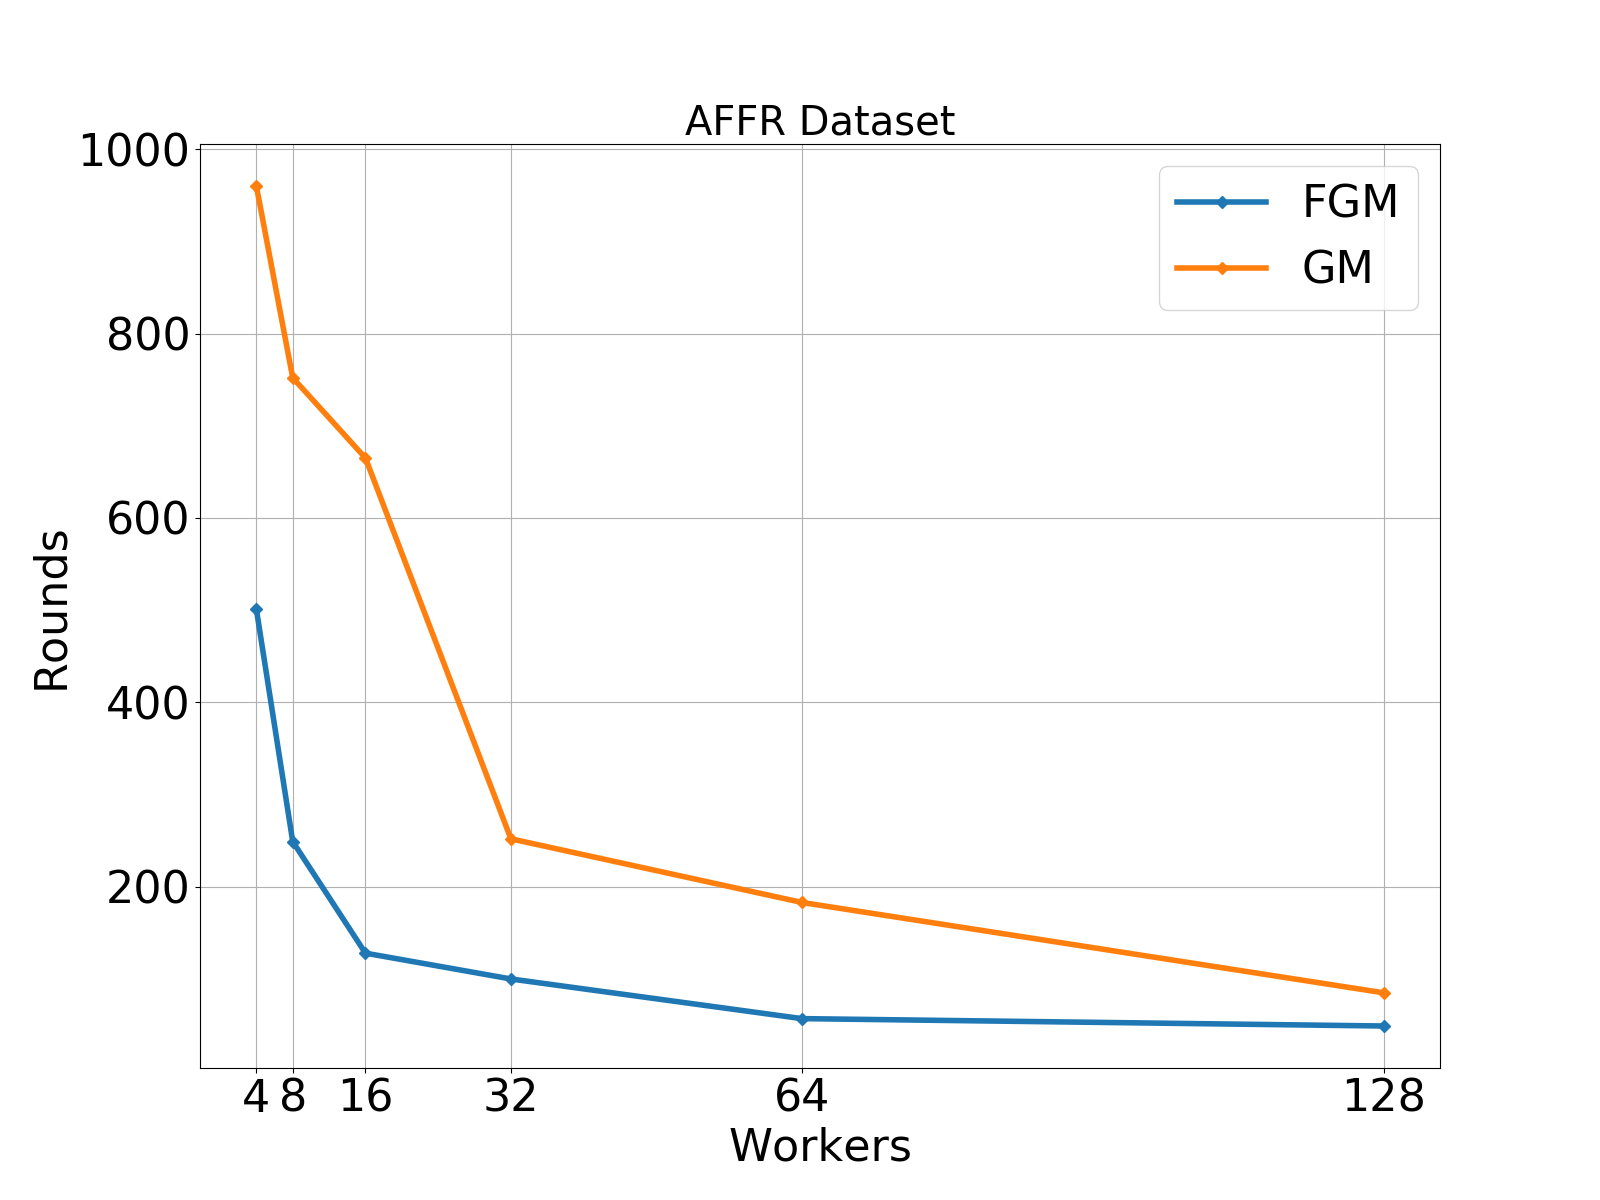
\includegraphics[width=3.9cm,height=3.5cm]{./images/results/amazon-plots/exp_Fig_3_2.png}}
        \subfigure{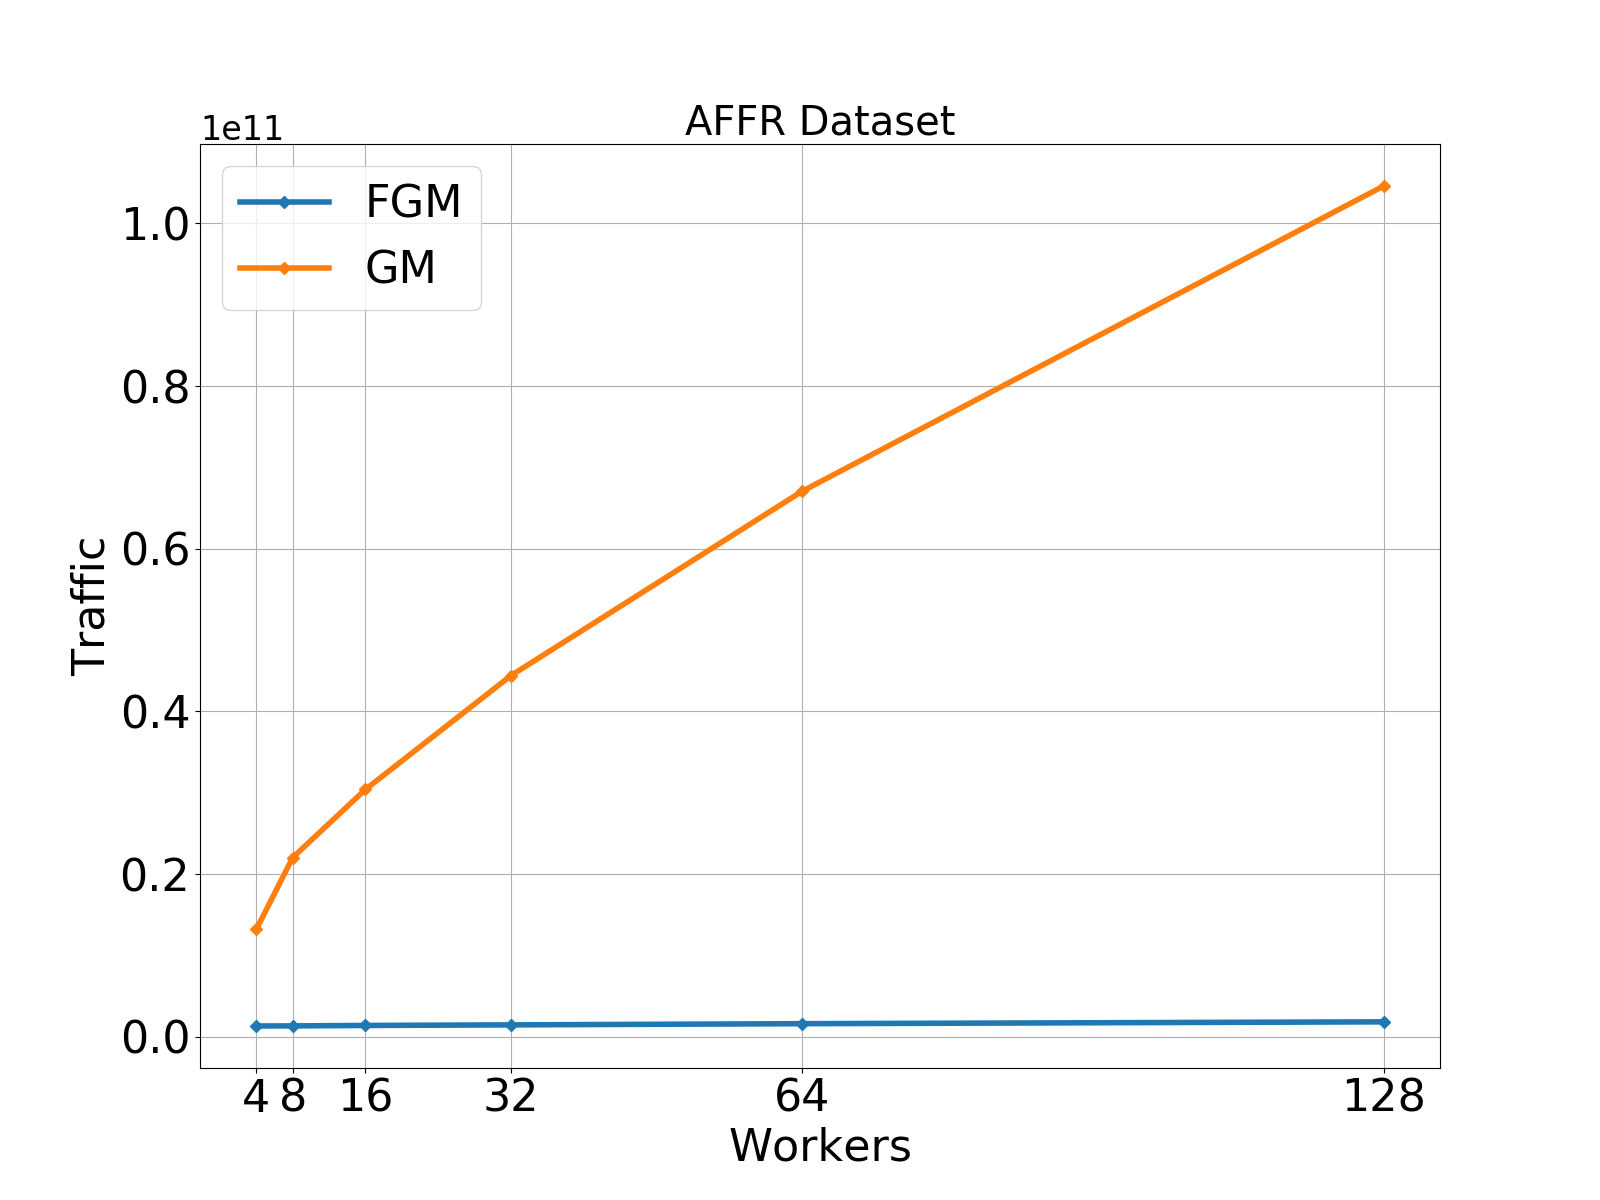
\includegraphics[width=3.9cm,height=3.5cm]{./images/results/amazon-plots/exp_Fig_3_3.png}}
        \label{fig:sfc-amazon-workers}
    \end{figure}
\end{frame}

\begin{frame}{Results (4) - Focusing on a specific case}
%    \begin{itemize}
%        \item{A comment.}
%    \end{itemize}
%    \vspace{-0.35cm}
    \begin{figure}
        \subfigure{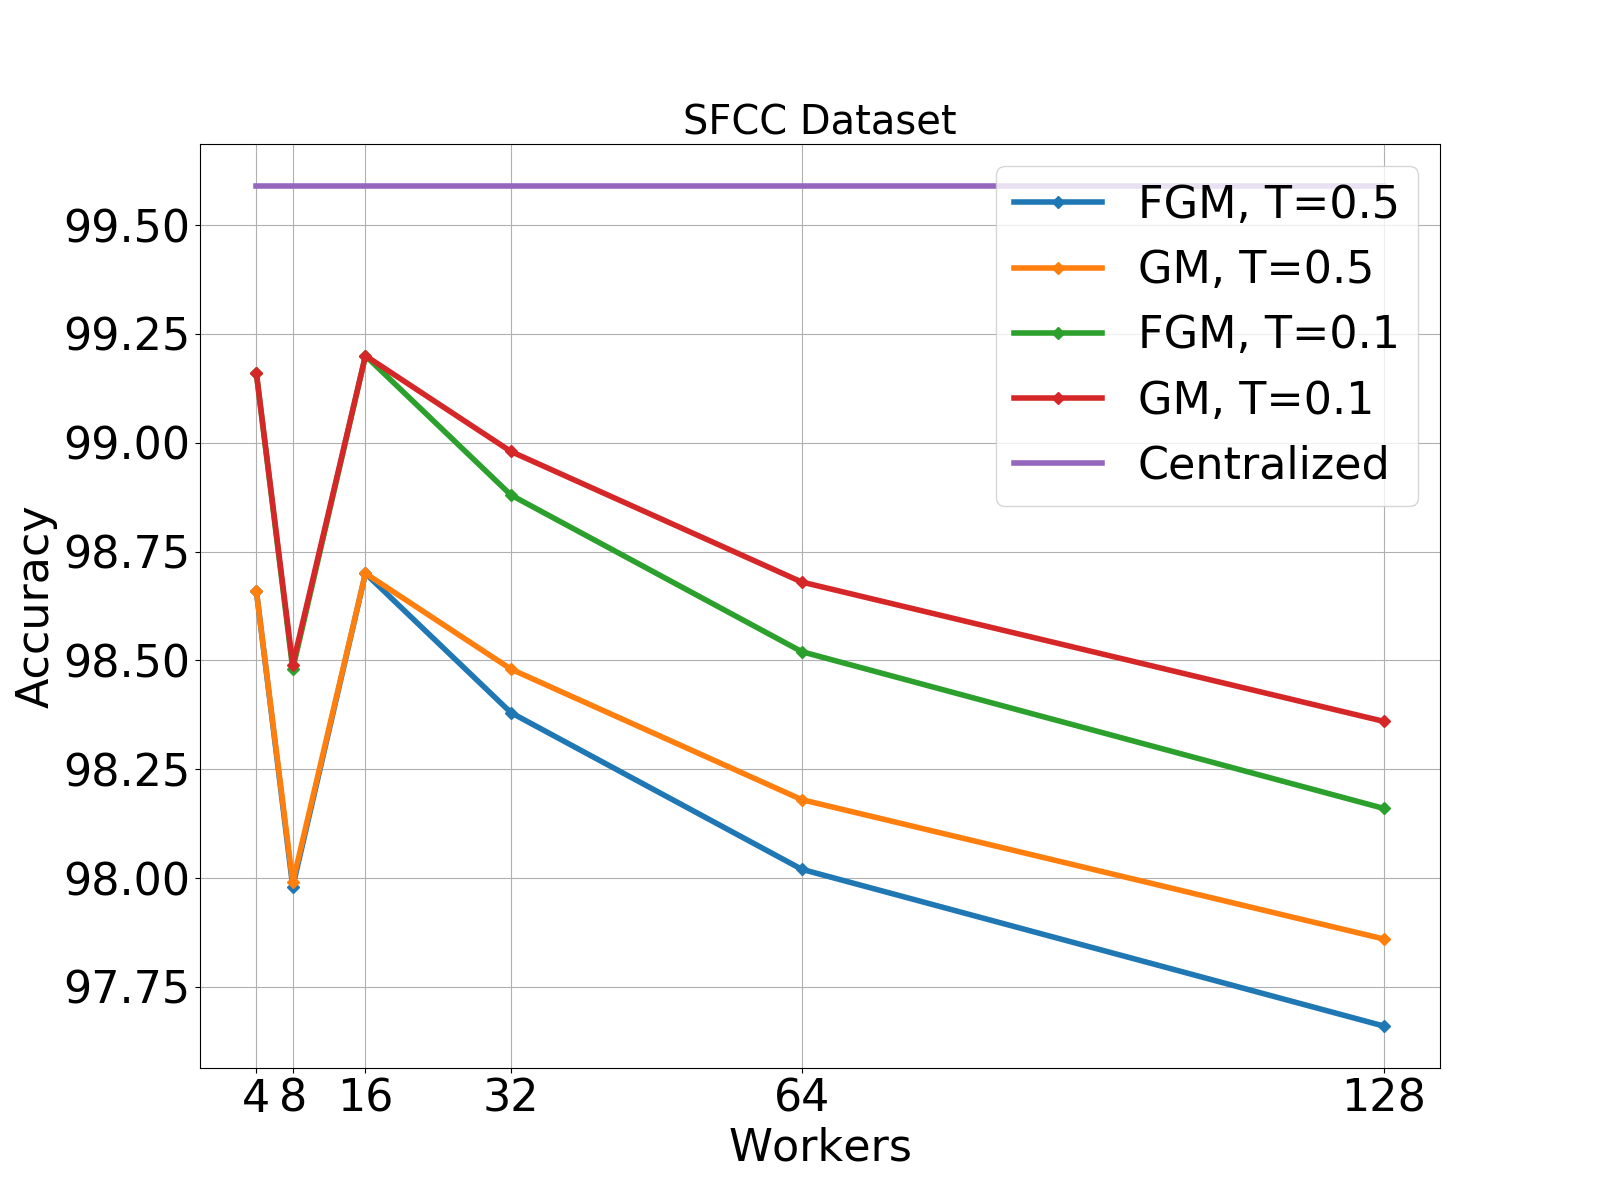
\includegraphics[width=5.2cm,height=3.7cm]{./images/results/sfc-plots/exp_Fig_3_1_b.png}}
        \subfigure{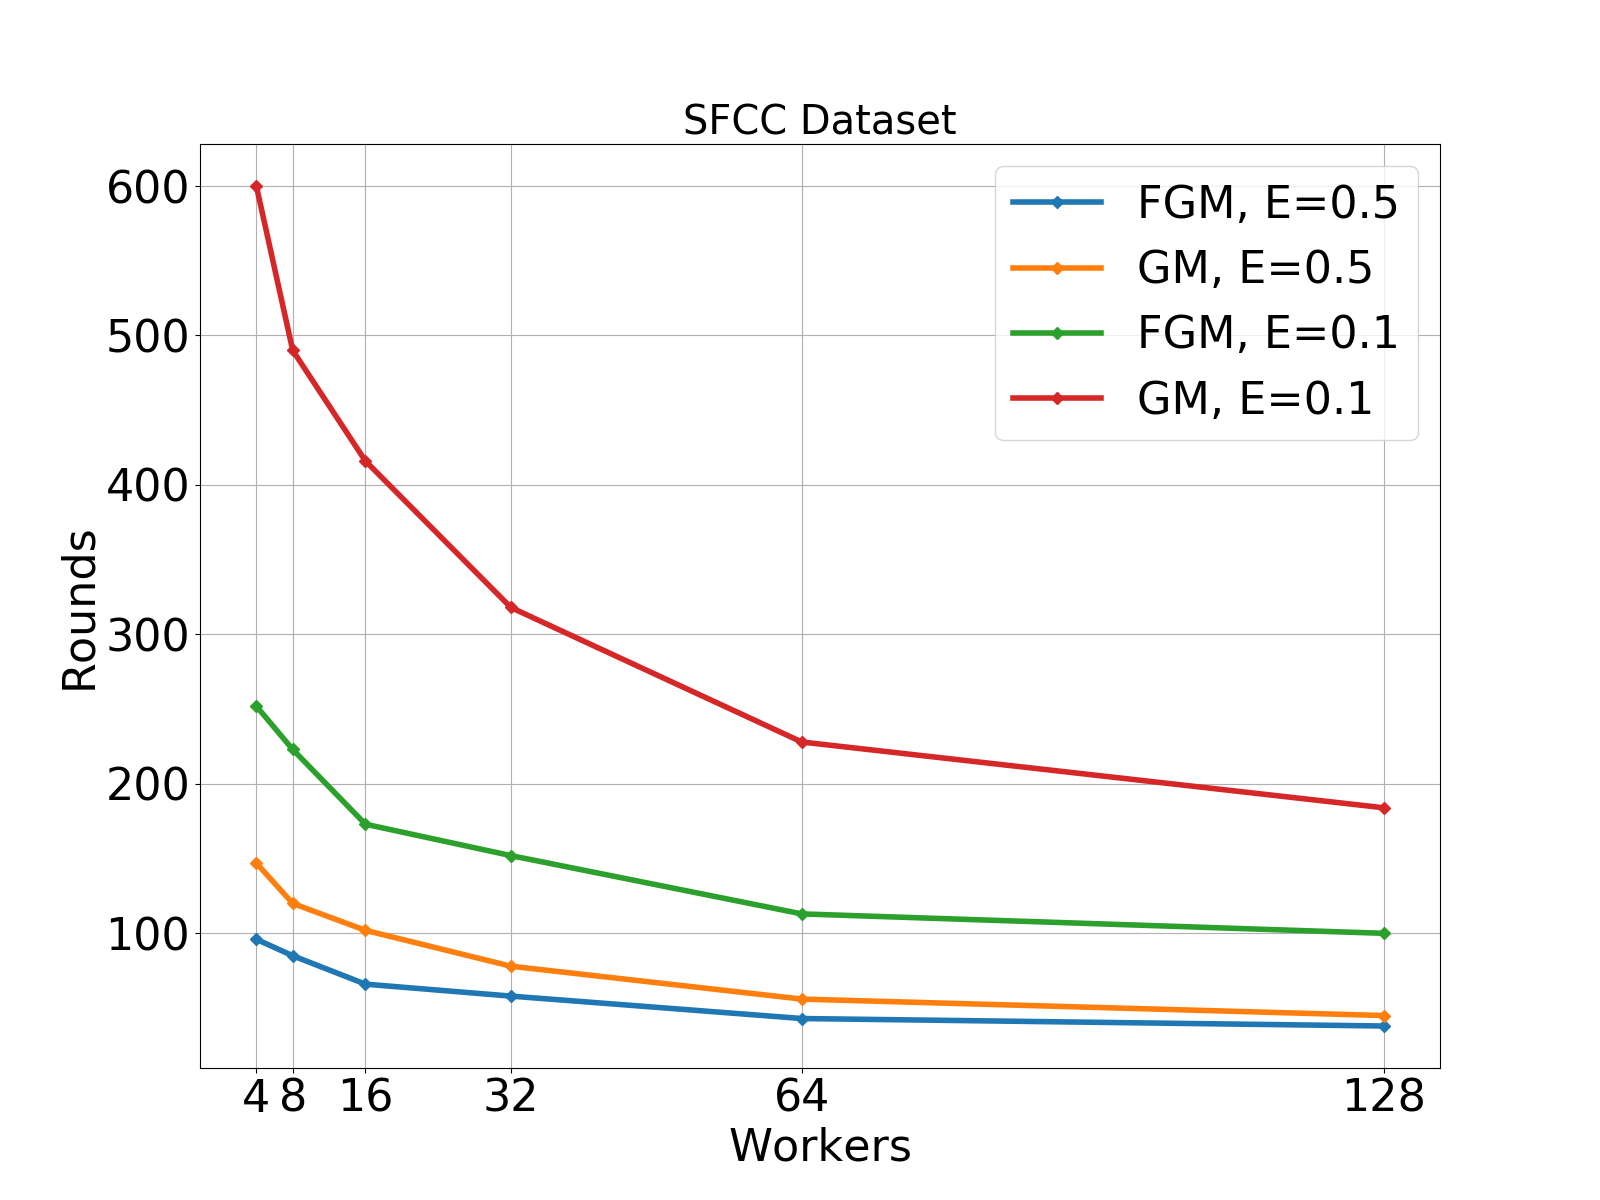
\includegraphics[width=5.2cm,height=3.7cm]{./images/results/sfc-plots/exp_Fig_3_2_b.png}}
        \subfigure{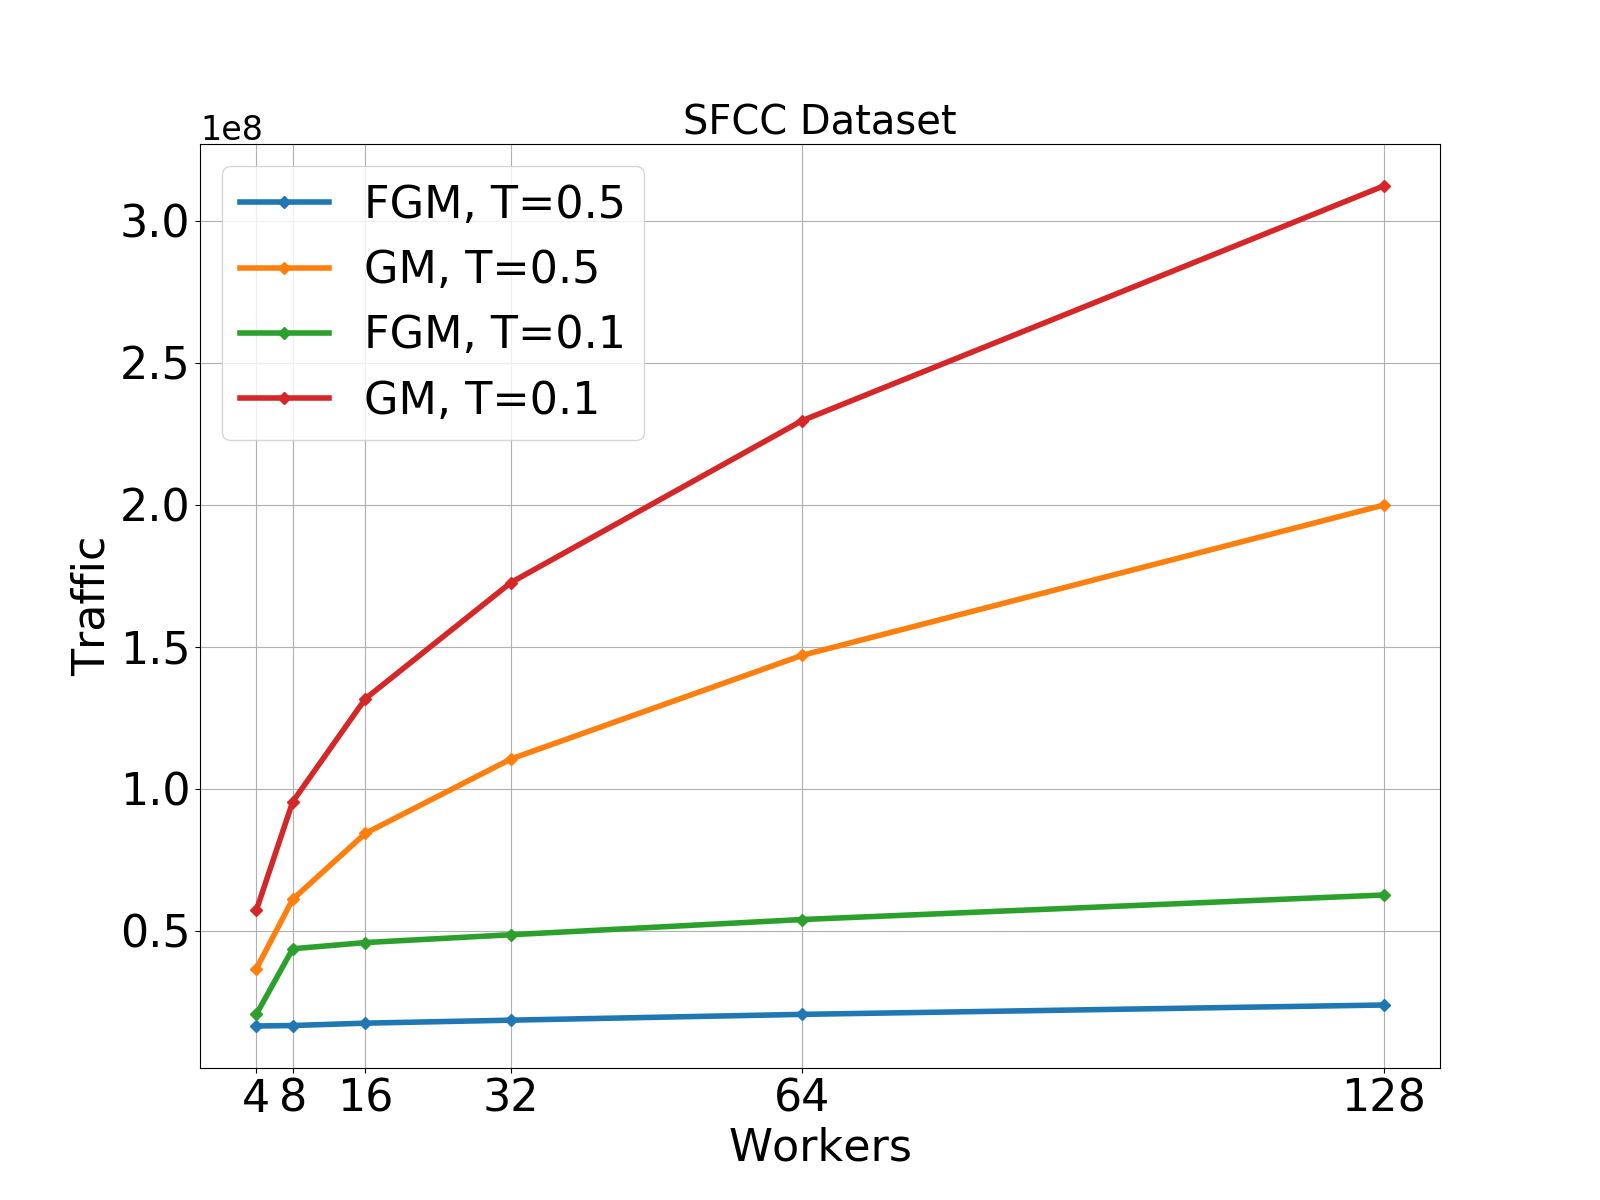
\includegraphics[width=5.2cm,height=3.7cm]{./images/results/sfc-plots/exp_Fig_3_3_b.png}}
        \label{fig:sfc_thres_workers}
    \end{figure}
\end{frame}

\subsection{Safe Functions Comparison}\label{subsec:safe-functions-comparison}

\begin{frame}{Safe Zone Problem}
    \setbeamertemplate{itemize items}[circle]
    \begin{itemize}
        \item{This time, we compare the two safe functions using the\\ \emph{same} protocol (\textbf{FGM}).}
        \item{The two safe functions are,}
        \vspace{0.2cm}
        \item[]{
        \begin{block}{Safe Function 1 (SF1) - \emph{'Simple norm'}}
            $\phi(\pmb{X_i},\pmb{E}) = ||\pmb{X_i}-\pmb{E}||_2^2 - T$
        \end{block}}
        \vspace{0.3cm}
        \begin{block}{Safe Function 2 (SF2) - \emph{'Spherical cap'}}
            $\phi(\pmb{X_i},\pmb{E}) = \max\{-T||\pmb{E}|| - \pmb{X_i}\frac{\pmb{E}}{\pmb{||E||}}, ||\pmb{X_i}+\pmb{E}|| - (1+T)||\pmb{E}||\}$
        \end{block}
    \end{itemize}
\end{frame}

\begin{frame}{Results (1) - Accuracy}
    \setbeamertemplate{itemize items}[circle]
    \begin{itemize}
        \item{\textbf{SF1} achieves a little bit \textbf{better} accuracy.}
    \end{itemize}
    \vspace{-0.35cm}
    \begin{figure}
        \subfigure{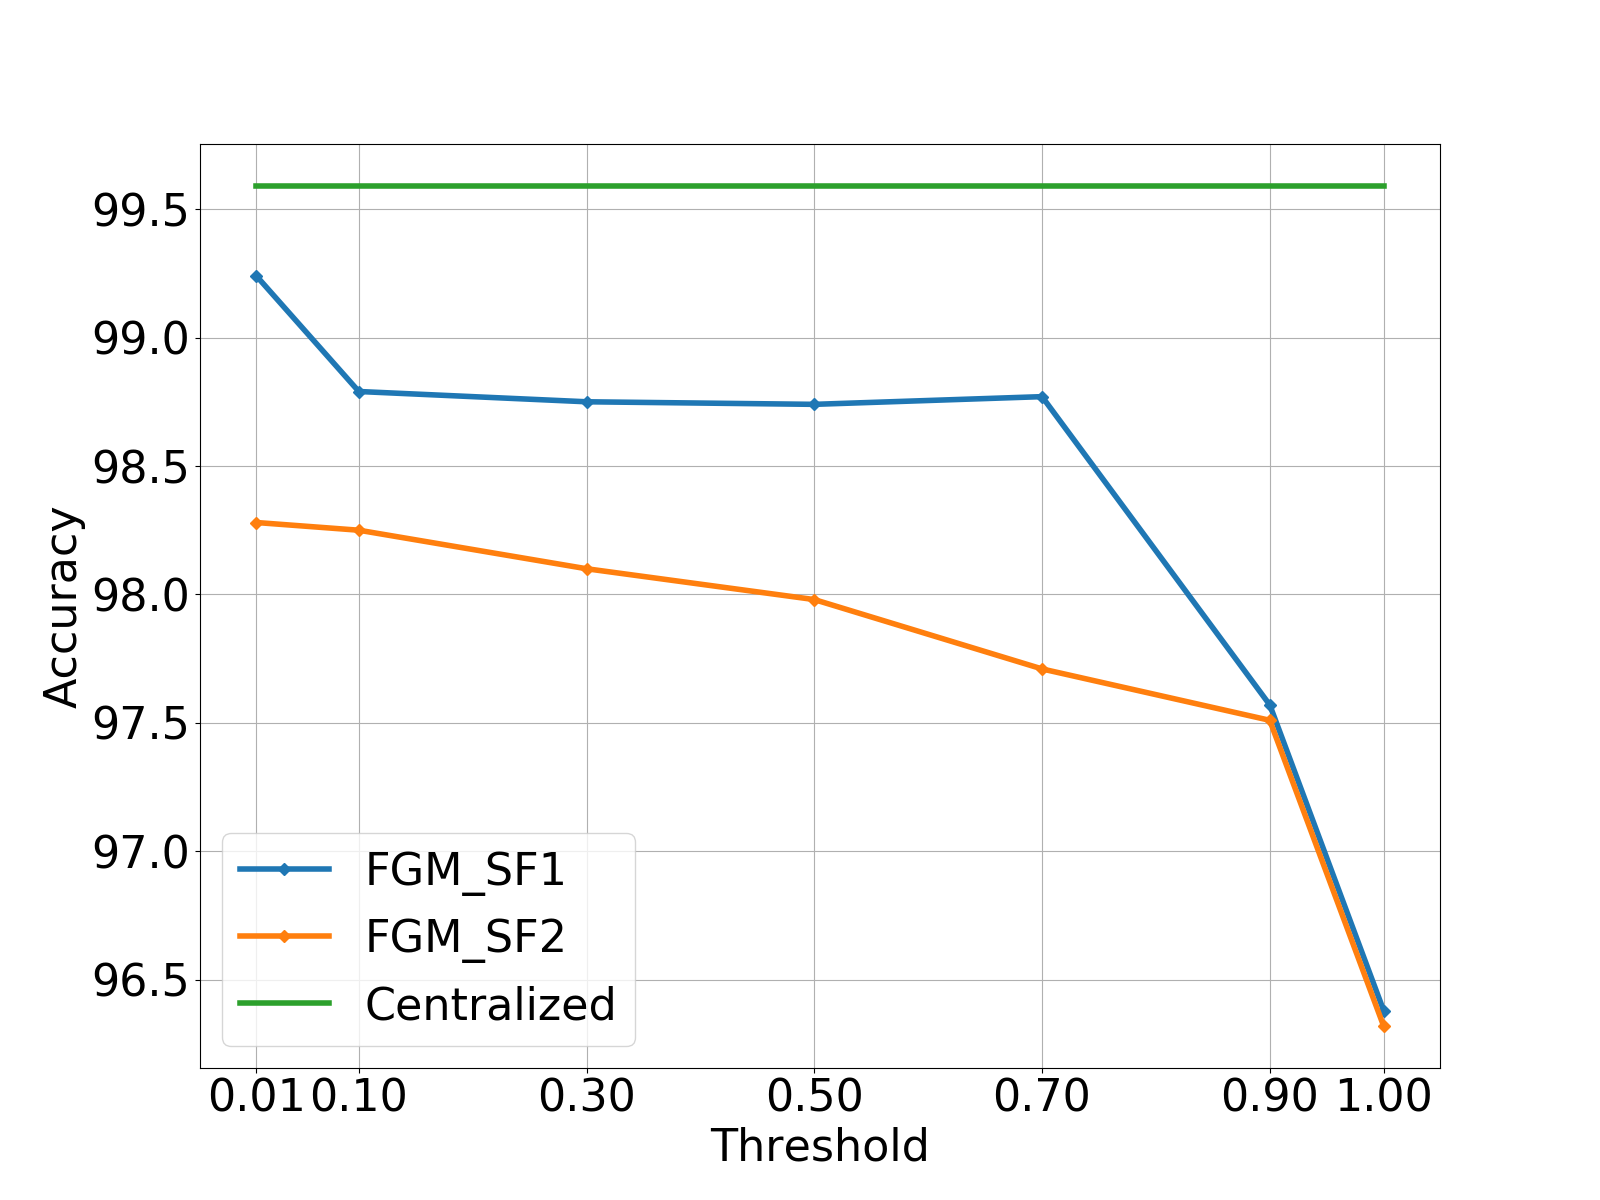
\includegraphics[width=5.2cm,height=3.7cm]{./images/results/sf-comp/exp_Fig_1_1.png}}
        \subfigure{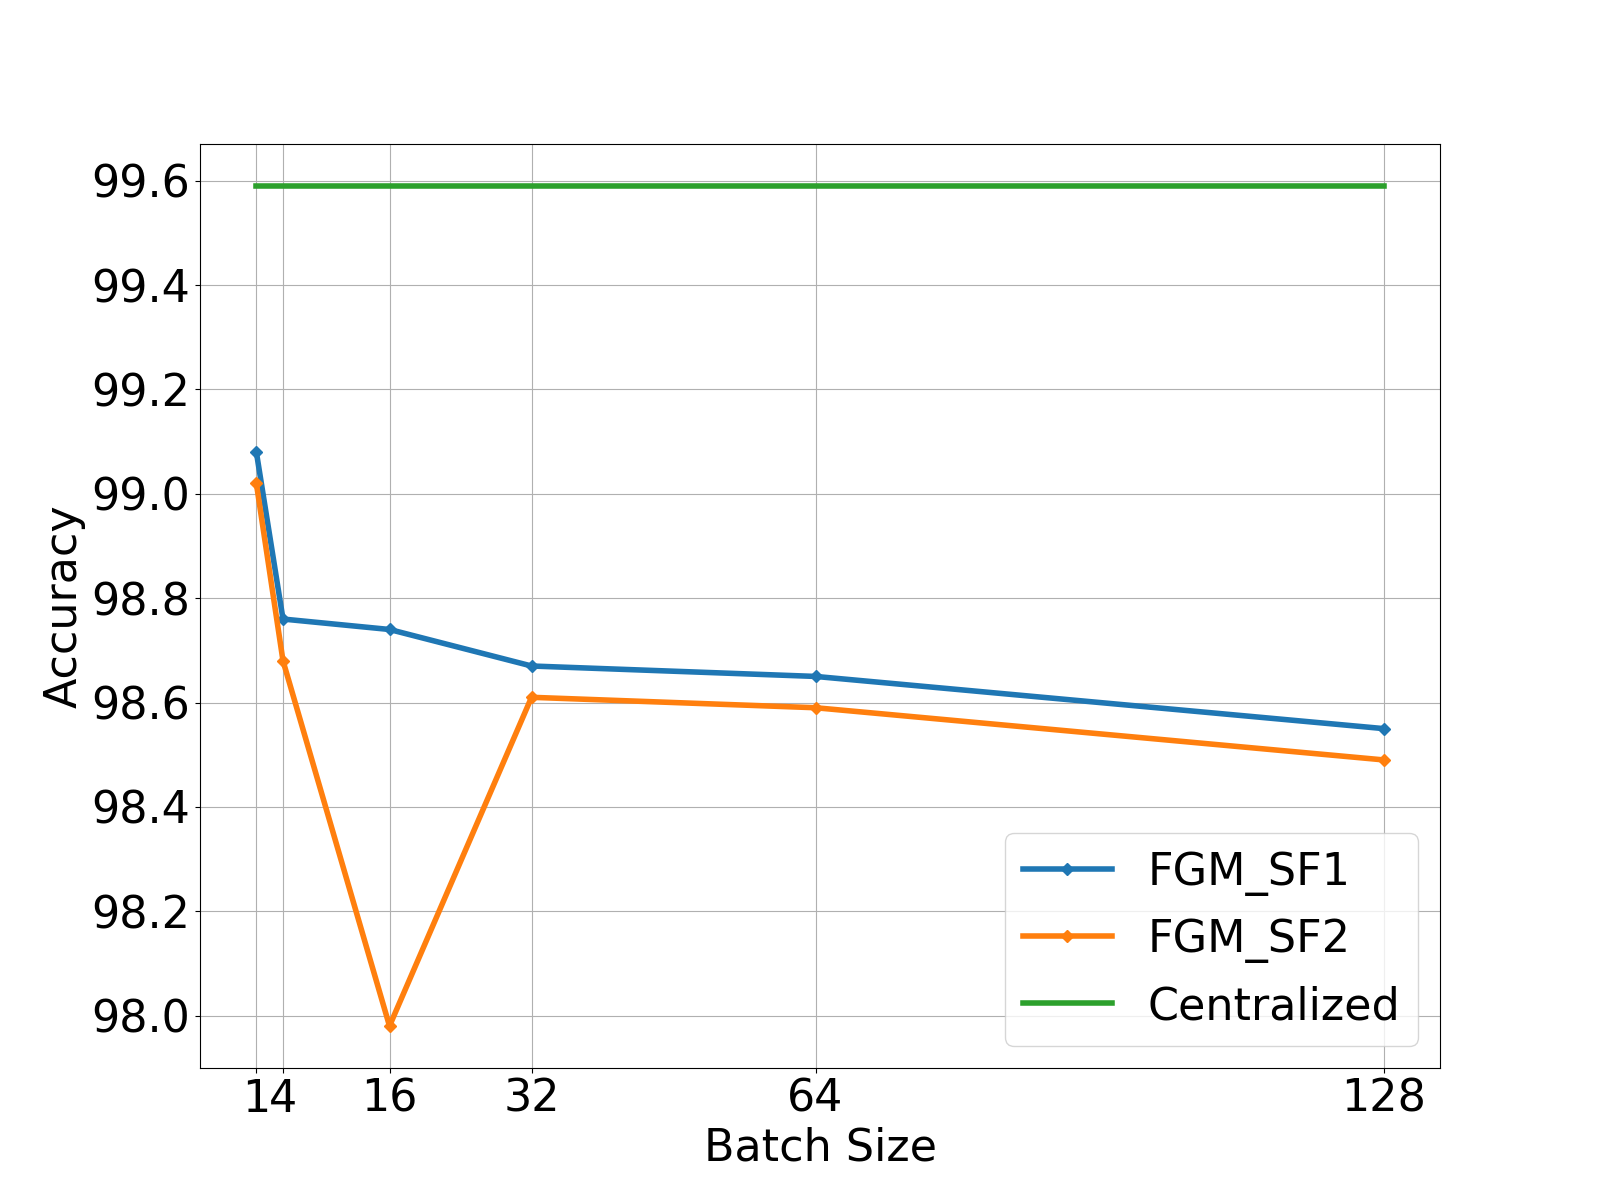
\includegraphics[width=5.2cm,height=3.7cm]{./images/results/sf-comp/exp_Fig_2_1.png}}
        \subfigure{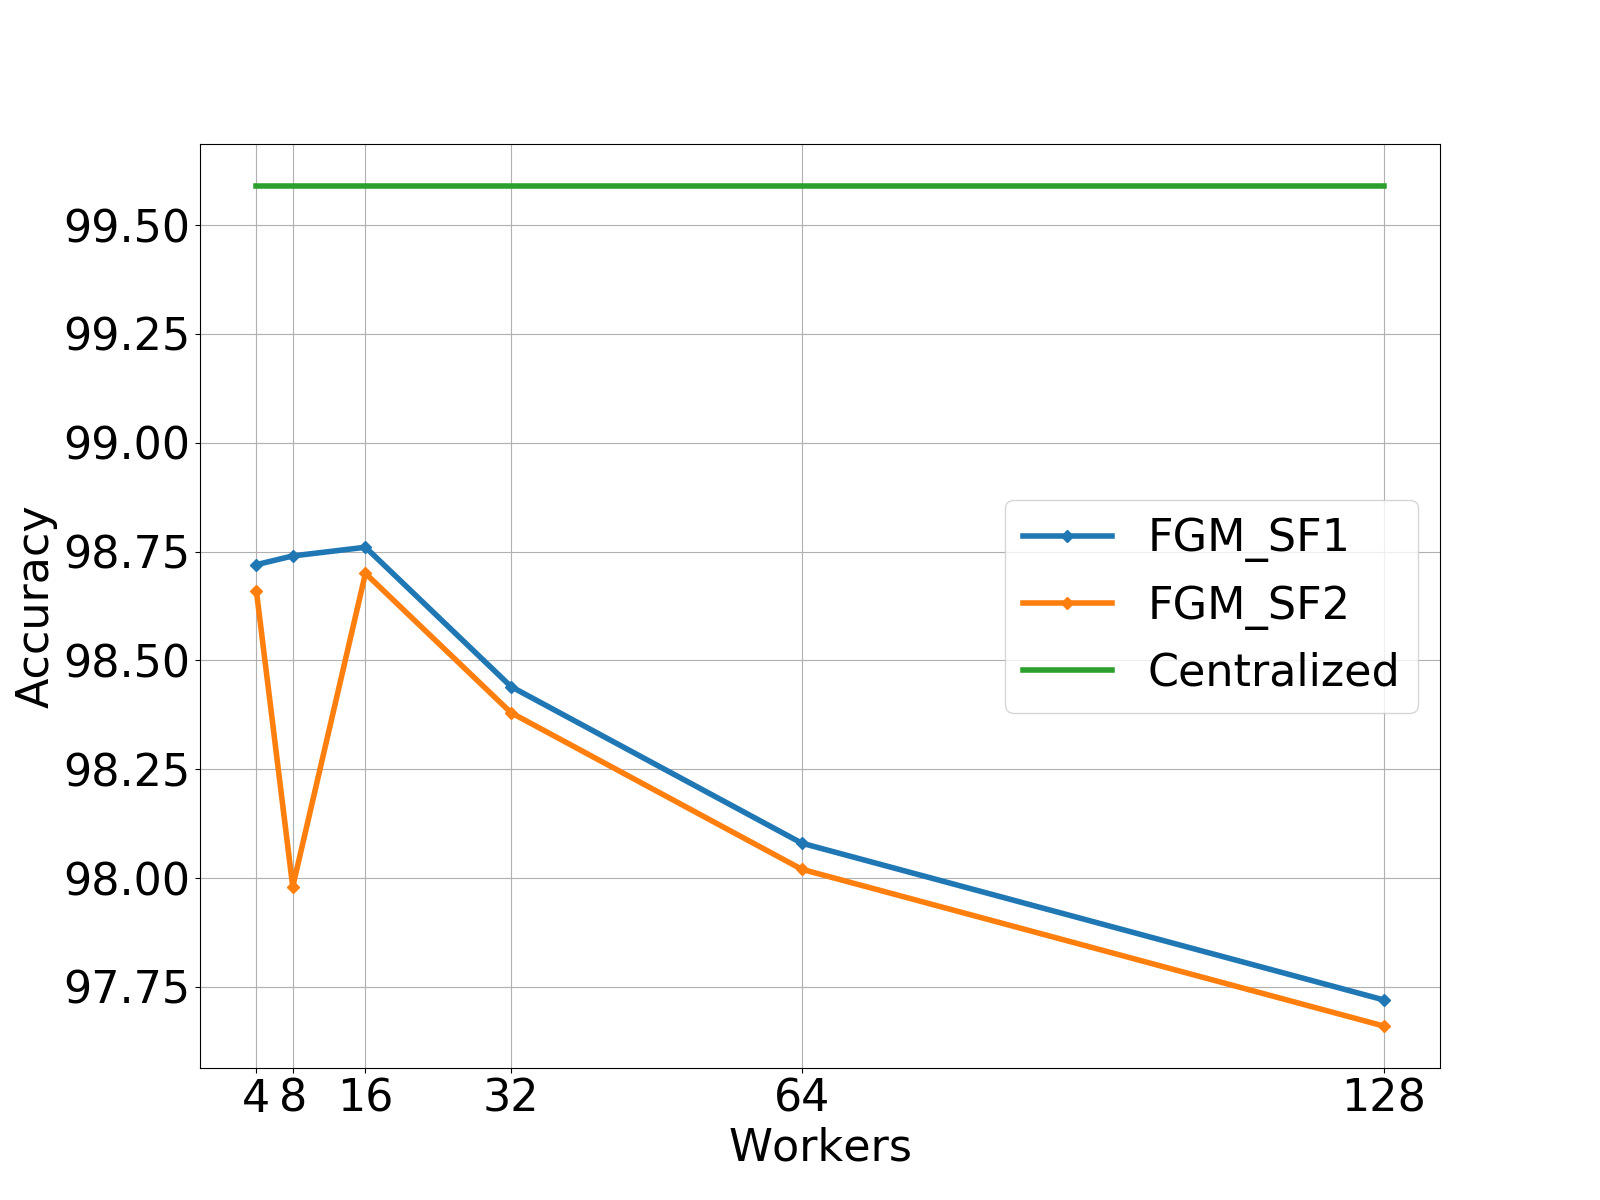
\includegraphics[width=5.2cm,height=3.7cm]{./images/results/sf-comp/exp_Fig_3_1.png}}
        \label{fig:sf_acc}
    \end{figure}
\end{frame}

\begin{frame}{Results (2) - Number of rounds}
%    \setbeamertemplate{itemize items}[circle]
%    \begin{itemize}
%        \item{A comment}
%    \end{itemize}
%    \vspace{-0.35cm}
    \begin{figure}
        \subfigure{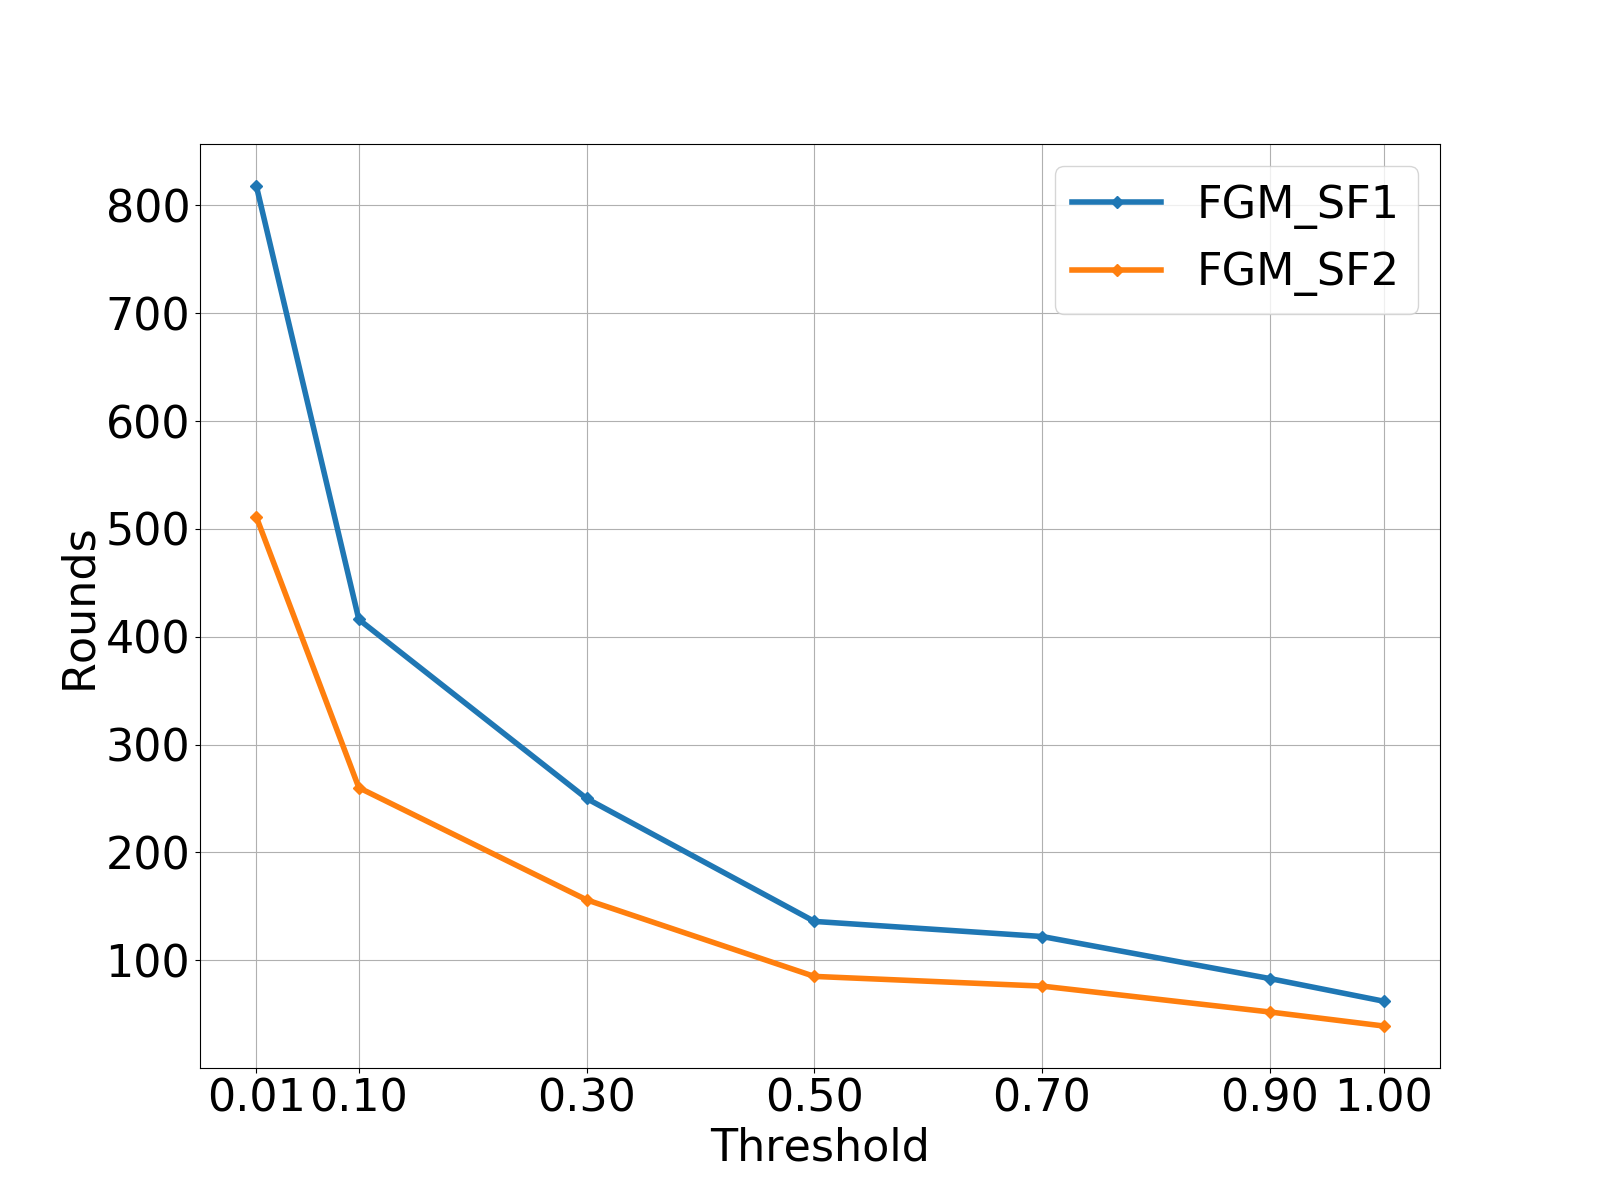
\includegraphics[width=5.2cm,height=3.7cm]{./images/results/sf-comp/exp_Fig_1_2.png}}
        \subfigure{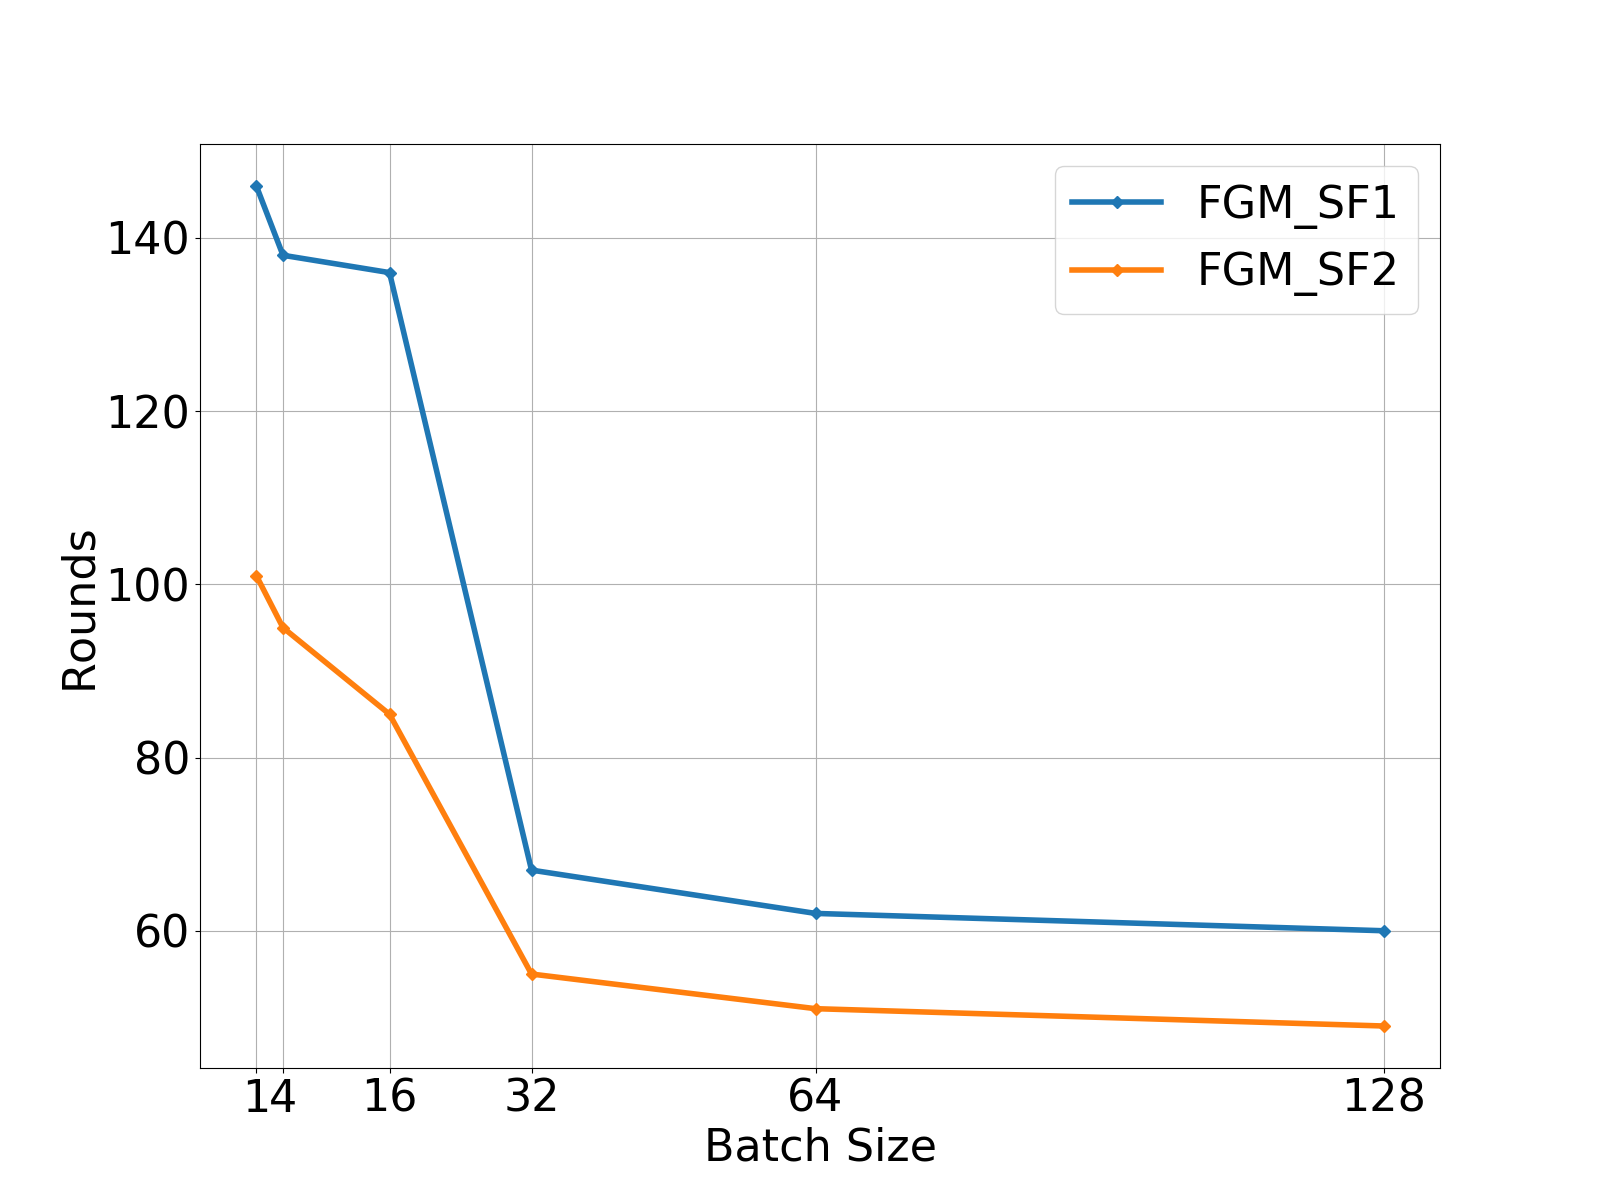
\includegraphics[width=5.2cm,height=3.7cm]{./images/results/sf-comp/exp_Fig_2_2.png}}
        \subfigure{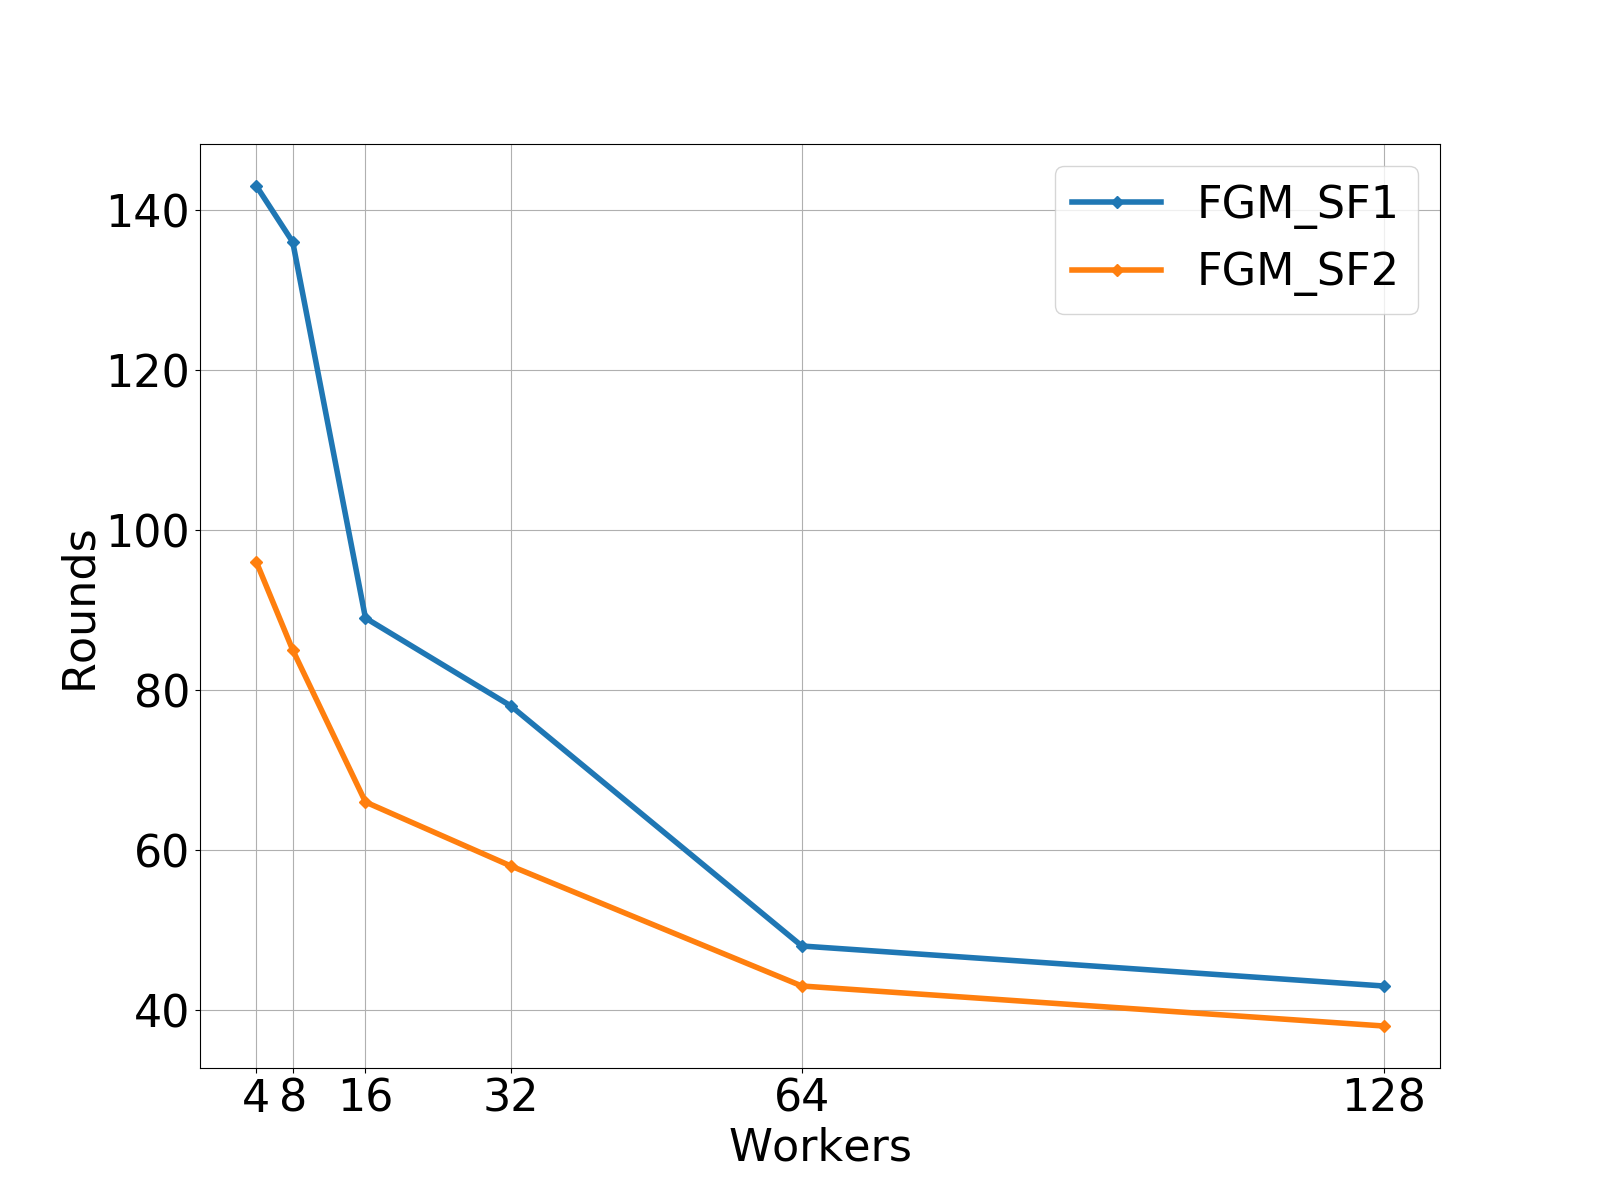
\includegraphics[width=5.2cm,height=3.7cm]{./images/results/sf-comp/exp_Fig_3_2.png}}
        \label{fig:sf_rnds}
    \end{figure}
\end{frame}

\begin{frame}{Results (3) - Scalabilty Analysis}
    \setbeamertemplate{itemize items}[circle]
    \begin{itemize}
        \item{\textbf{SF2} is more \textbf{efficient} by up to 56\%.}
    \end{itemize}
    \vspace{-0.35cm}
    \begin{figure}
        \subfigure{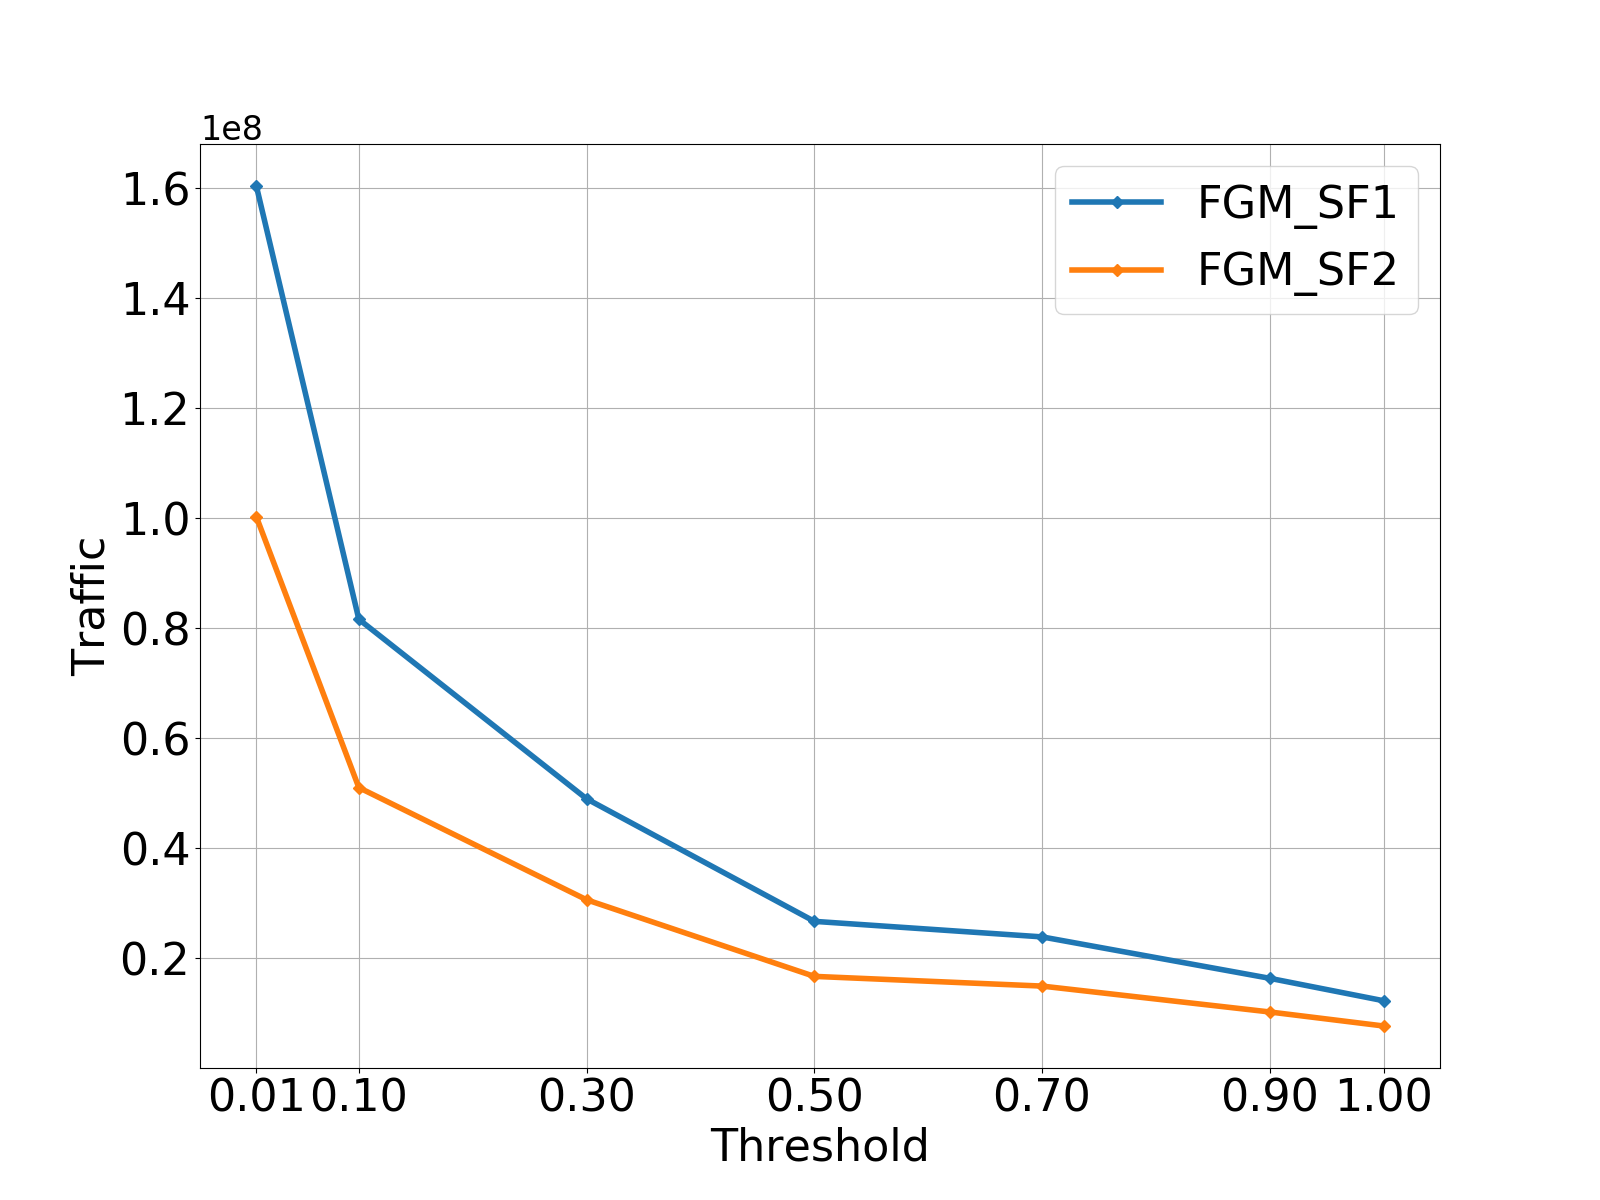
\includegraphics[width=5.2cm,height=3.7cm]{./images/results/sf-comp/exp_Fig_1_3.png}}
        \subfigure{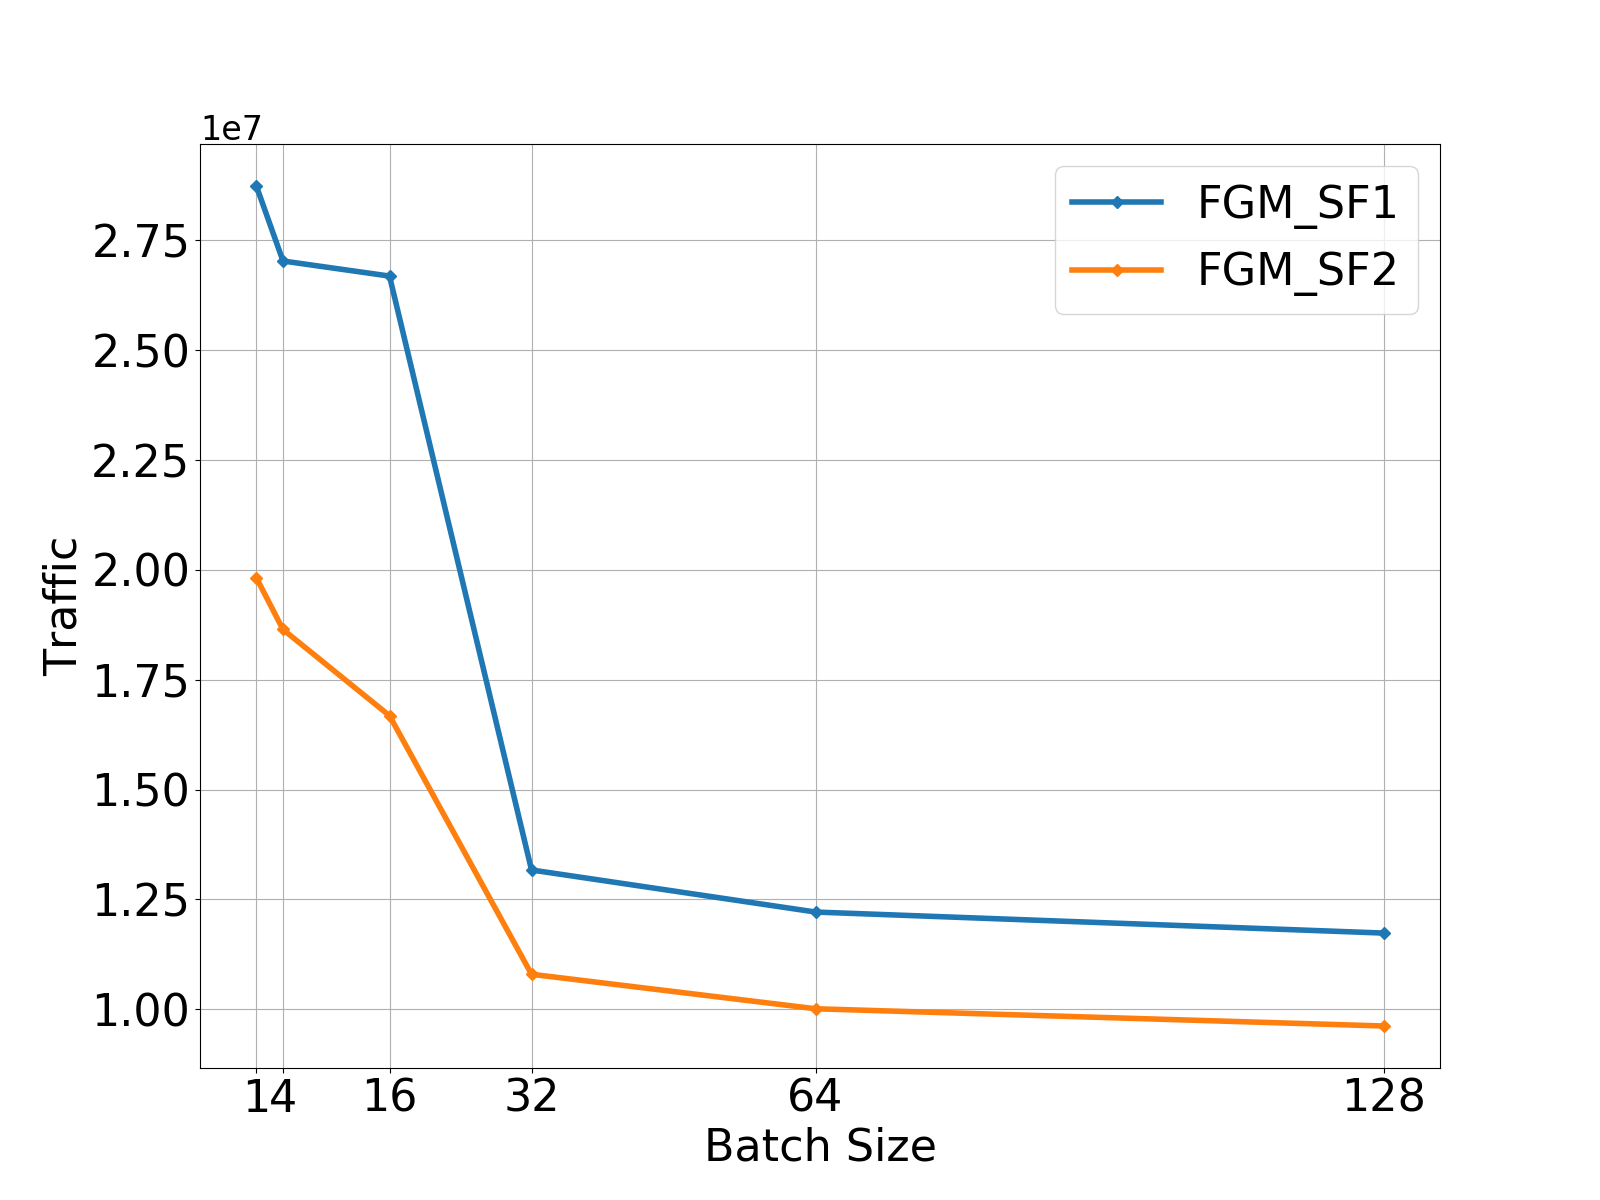
\includegraphics[width=5.2cm,height=3.7cm]{./images/results/sf-comp/exp_Fig_2_3.png}}
        \subfigure{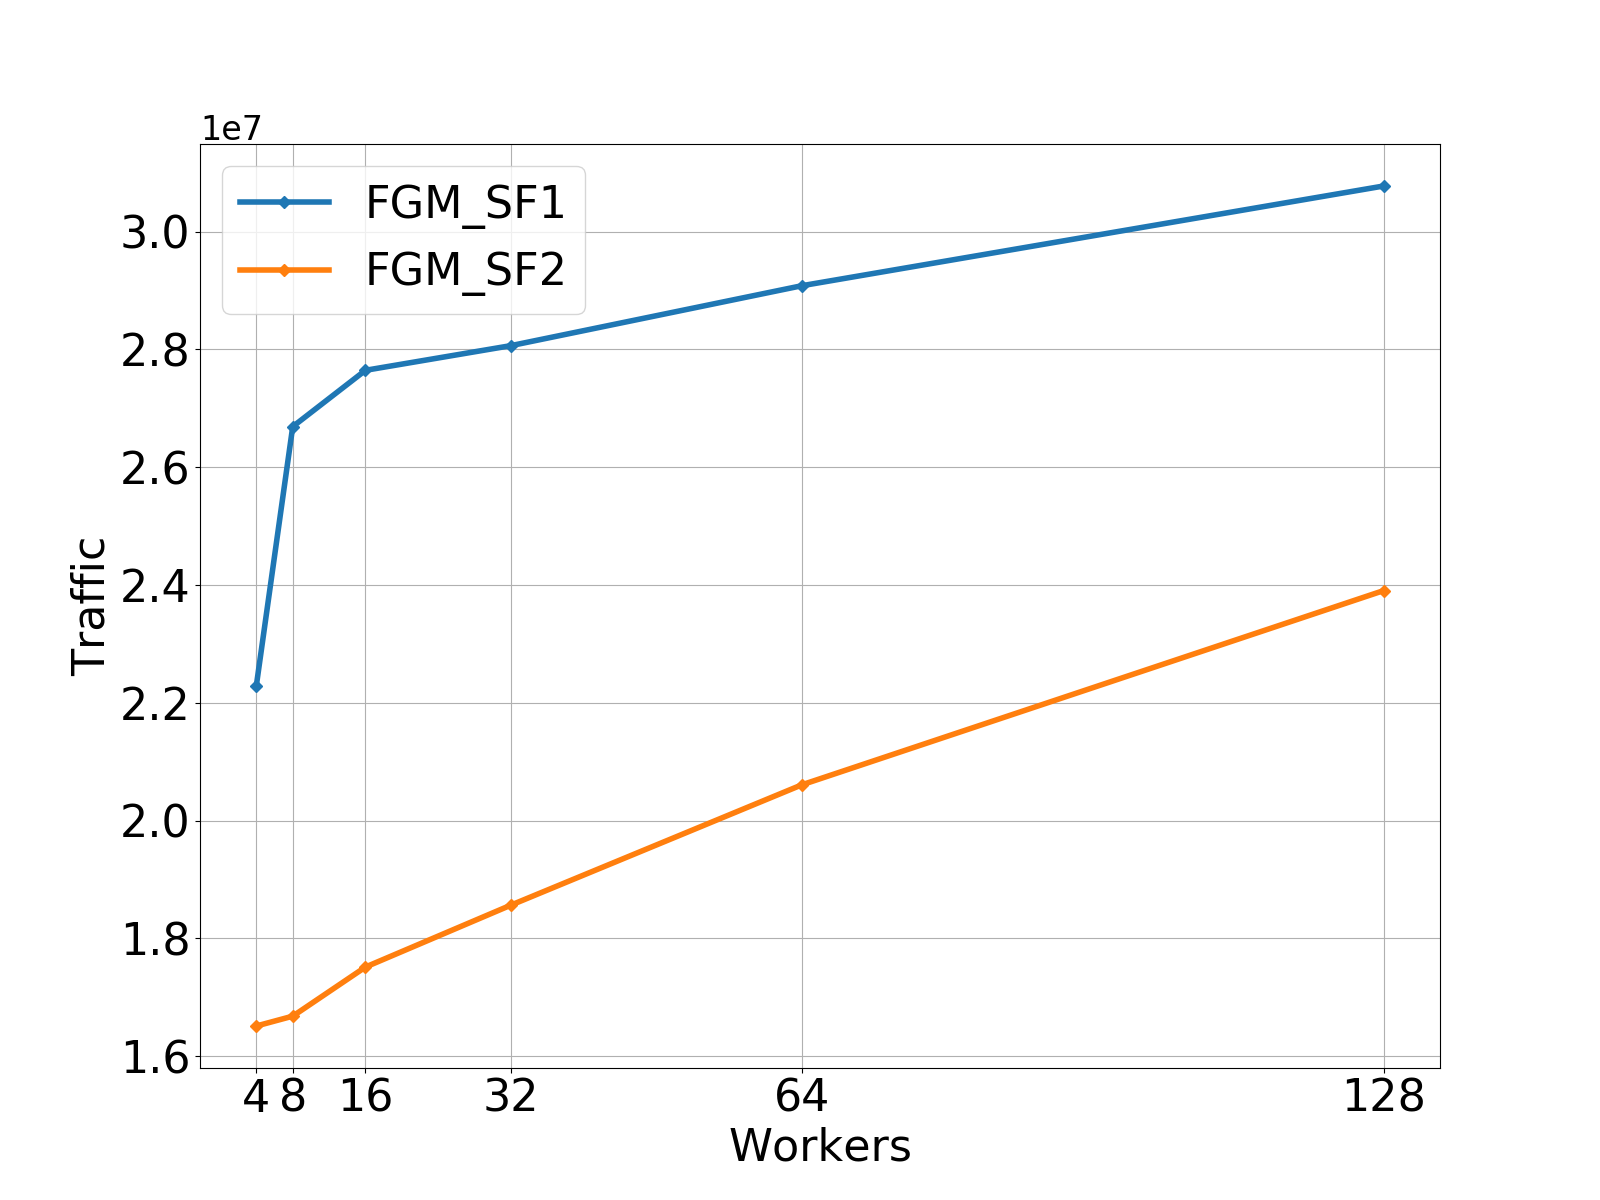
\includegraphics[width=5.2cm,height=3.7cm]{./images/results/sf-comp/exp_Fig_3_3.png}}
        \label{fig:sf_trff}
    \end{figure}
\end{frame}
    \chapter{Conclusions}\label{ch:conclusions}

\section{Contribution}\label{sec:conclusion}

Our recommended method for distributed DL achieves high predictive performance, yet needs essentially less communication than GM\@.
Furthermore, the method handles not only the learning algorithm but also the optimizer as black-boxes.
In this work, I proved that FGM is better than GM for distributed DL learning and especially using LSTM networks, a subset of the Recurrent Neural Networks.
I tested this architecture on solving two types of problems, classification, and sentiment analysis.
In both cases, the results were impressive.
But if we have to choose one of these two for which the architecture is more suitable, the answer is the NLP problem.
Taking into account the difficulty of both problems, our architecture reacted almost in the same way in both cases.

In the second phase, I compared the two functions with each other.
The results revealed that SF2 is much cheaper than SF1 in terms of network cost, but the latter achieves better accuracy on the prediction.
Of course, this difference is not so important as to make us prefer it.
Therefore, sacrificing minimal accuracy in the model, we choose SF2 as the best for distributed deep learning.

\section{Future Work}\label{sec:future-work}

In this work, I simulated a scenario calculating the network traffic cost of the training process of RNN by the GM and FGM protocol.
We know this time in practice that the FGM protocol is more efficient than GM.
Thus, a future direction would be an actual system that uses FGM to train these networks.
Recently, Sofia Kampioti~\cite{kampioti_sofia__thesis_2020} implemented such a system to train an ML model for classification purposes using the Support Vector Machines (SVM) algorithm.

Another future direction would be the usage of the rebalancing version of FGM on RNN training.
Using the rebalancing version, we can undoubtedly achieve much more efficient training concerning the network cost.

Last, in this project, we made offline learning.
Future work could attempt to make this process online, taking into consideration some meaning like Concept Drift.
An online learning algorithm can resolve some issues like concept changes.
To make this more specific, in this task I used the food reviews as training samples.
In an online learning system, we could change the concept of training samples to cloth reviews without accepting a large reduction in the forecast performance.


%%%% Bibliography
    \printbibliography[title={References}]~\nocite{*}

% Appendices
    \appendix
    \chapter{Abbreviations}\label{ch:abbreviations}

\begin{tabular}{ll}
    \textbf{ML}   & Machine Learning                   \\
    \textbf{AI}   & Artificial Intelligence            \\
    \textbf{RL}   & Reinforcement Learning             \\
    \textbf{MDP}  & Markov Decision Process            \\
    \textbf{DL}   & Deep Learning                      \\
    \textbf{DML}  & Distributed Machine Learning       \\
    \textbf{ANN}  & Artificial Neural Network          \\
    \textbf{NN}   & Neural network                     \\
    \textbf{FFNN} & Feed-Forward Neural Network        \\
    \textbf{MSE}  & Mean Squared Error                 \\
    \textbf{BP}   & Backpropagation                    \\
    \textbf{DNN}  & Deep Neural Network                \\
    \textbf{GD}   & Gradient Descent                   \\
    \textbf{CNN}  & Convolutional Neural Network       \\
    \textbf{RNN}  & Recurrent Neural Network           \\
    \textbf{BPTT} & Backpropagation Through Time       \\
    \textbf{SGD}  & Stochastic Gradient Descent        \\
    \textbf{LSTM} & Long Short Term Memory             \\
    \textbf{GM}   & Geometric Monitoring               \\
    \textbf{FGM}  & Functional Geometric Monitoring    \\
    \textbf{NLP}  & Natural Language Processing        \\
    \textbf{SFCC} & San Francisco Crime Classification \\
    \textbf{AFFR} & Amazon Fine Food Reviews           \\
    \textbf{SVM}  & Support Vector Machines            \\
\end{tabular}
    \chapter{Detailed Experimental Results}\label{ch:detailed-experimental-results}


\section{SFCC Dataset Results}\label{sec:sfcc-dataset-results}

\begin{table}[H]
    \begin{tabular}{|c|c|c|c|c|c|c|c|}
        \hline
        \textbf{id}            & \textbf{Threshold}    & \textbf{Batch Size}   & \textbf{Workers}      & \textbf{Rounds}       & \textbf{Rebalances}   & \textbf{Accuracy}     & \textbf{Traffic (bytes)} \\
        \hline
        1                      & 0.01                  & 16                    & 8                     & 1296                  & 8424                  & 99.42                 & 660,214,152              \\
        2                      & 0.1                   & 16                    & 8                     & 781                   & 5075                  & 99.01                 & 397,758,650              \\
        3                      & 0.3                   & 16                    & 8                     & 589                   & 3827                  & 98.97                 & 299,949,146              \\
        4                      & 0.5                   & 16                    & 8                     & 192                   & 1248                  & 98.74                 & 97,809,504               \\
        5                      & 0.7                   & 16                    & 8                     & 149                   & 968                   & 98.77                 & 75,802,366               \\
        6                      & 0.9                   & 16                    & 8                     & 98                    & 635                   & 98.25                 & 49,719,832               \\
        7                      & 1                     & 16                    & 8                     & 67                    & 437                   & 97.36                 & 34,233,326               \\
        \hline
        \multicolumn{1}{|l|}{} & \multicolumn{1}{l|}{} & \multicolumn{1}{l|}{} & \multicolumn{1}{l|}{} & \multicolumn{1}{l|}{} & \multicolumn{1}{l|}{} & \multicolumn{1}{l|}{} & \multicolumn{1}{l|}{}    \\
        \hline
        8                      & 0.5                   & 1                     & 8                     & 222                   & 1443                  & 99.18                 & 113,015,826              \\
        9                      & 0.5                   & 4                     & 8                     & 198                   & 1235                  & 98.78                 & 96,765,185               \\
        10                     & 0.5                   & 16                    & 8                     & 192                   & 1248                  & 98.74                 & 97,809,504               \\
        11                     & 0.5                   & 32                    & 8                     & 78                    & 510                   & 98.67                 & 39,938,881               \\
        12                     & 0.5                   & 64                    & 8                     & 76                    & 495                   & 98.65                 & 38,797,770               \\
        13                     & 0.5                   & 128                   & 8                     & 74                    & 480                   & 98.55                 & 37,656,659               \\
        \hline
        \multicolumn{1}{|l|}{} & \multicolumn{1}{l|}{} & \multicolumn{1}{l|}{} & \multicolumn{1}{l|}{} & \multicolumn{1}{l|}{} & \multicolumn{1}{l|}{} & \multicolumn{1}{l|}{} & \multicolumn{1}{l|}{}    \\
        \hline
        14                     & 0.5                   & 16                    & 4                     & 198                   & 1291                  & 98.72                 & 49,516,061               \\
        15                     & 0.5                   & 16                    & 8                     & 192                   & 1248                  & 98.74                 & 97,809,504               \\
        16                     & 0.5                   & 16                    & 16                    & 138                   & 895                   & 98.76                 & 113,886,941              \\
        17                     & 0.5                   & 16                    & 32                    & 105                   & 684                   & 98.54                 & 149,191,893              \\
        18                     & 0.5                   & 16                    & 64                    & 76                    & 491                   & 98.24                 & 198,425,217              \\
        19                     & 0.5                   & 16                    & 128                   & 61                    & 396                   & 97.92                 & 269,858,295              \\
        \hline
    \end{tabular}
    \caption{(SFCC) Training by GM protocol using as safe function the simple norm}
    \label{tab:table-gm-sf1-class-exp}
\end{table}

\newpage

\begin{table}[H]
    \begin{tabular}{|c|c|c|c|c|c|c|c|}
        \hline
        \textbf{id}            & \textbf{Threshold}    & \textbf{Batch Size}   & \textbf{Workers}      & \textbf{Rounds}       & \textbf{Rebalances}   & \textbf{Accuracy}     & \textbf{Traffic (bytes)} \\
        \hline
        1                      & 0.01                  & 16                    & 8                     & 810                   & 5,265                 & 98.31                 & 412,633,845              \\
        2                      & 0.1                   & 16                    & 8                     & 488                   & 3,172                 & 98.29                 & 248,599,156              \\
        3                      & 0.3                   & 16                    & 8                     & 368                   & 2,392                 & 98.3                  & 187,468,216              \\
        4                      & 0.5                   & 16                    & 8                     & 120                   & 780                   & 97.99                 & 61,130,940               \\
        5                      & 0.7                   & 16                    & 8                     & 93                    & 605                   & 97.81                 & 47,376,479               \\
        6                      & 0.9                   & 16                    & 8                     & 61                    & 397                   & 97.63                 & 31,074,895               \\
        7                      & 1                     & 16                    & 8                     & 42                    & 273                   & 96.45                 & 21,395,829               \\
        \hline
        \multicolumn{1}{|l|}{} & \multicolumn{1}{l|}{} & \multicolumn{1}{l|}{} & \multicolumn{1}{l|}{} & \multicolumn{1}{l|}{} & \multicolumn{1}{l|}{} & \multicolumn{1}{l|}{} & \multicolumn{1}{l|}{}    \\
        \hline
        8                      & 0.5                   & 1                     & 8                     & 153                   & 995                   & 99.12                 & 77,941,949               \\
        9                      & 0.5                   & 4                     & 8                     & 131                   & 852                   & 98.72                 & 66,734,610               \\
        10                     & 0.5                   & 16                    & 8                     & 120                   & 780                   & 97.99                 & 61,130,940               \\
        11                     & 0.5                   & 32                    & 8                     & 70                    & 455                   & 98.61                 & 35,659,715               \\
        12                     & 0.5                   & 64                    & 8                     & 68                    & 442                   & 98.59                 & 34,640,866               \\
        13                     & 0.5                   & 128                   & 8                     & 66                    & 429                   & 98.49                 & 33,622,017               \\
        \hline
        \multicolumn{1}{|l|}{} & \multicolumn{1}{l|}{} & \multicolumn{1}{l|}{} & \multicolumn{1}{l|}{} & \multicolumn{1}{l|}{} & \multicolumn{1}{l|}{} & \multicolumn{1}{l|}{} & \multicolumn{1}{l|}{}    \\
        \hline
        14                     & 0.5                   & 16                    & 4                     & 147                   & 956                   & 98.66                 & 36,678,564               \\
        15                     & 0.5                   & 16                    & 8                     & 120                   & 780                   & 97.99                 & 61,130,940               \\
        16                     & 0.5                   & 16                    & 16                    & 102                   & 663                   & 98.7                  & 84,360,697               \\
        17                     & 0.5                   & 16                    & 32                    & 78                    & 507                   & 98.48                 & 110,512,513              \\
        18                     & 0.5                   & 16                    & 64                    & 56                    & 364                   & 98.18                 & 146,981,642              \\
        19                     & 0.5                   & 16                    & 128                   & 45                    & 293                   & 97.86                 & 199,895,033              \\
        \hline
    \end{tabular}
    \caption{(SFCC) Training by GM protocol using as safe function the spherical cap}
    \label{tab:table-gm-sf2-class-exp}
\end{table}

\newpage

\begin{table}[H]
    \begin{tabular}{|c|c|c|c|c|c|c|c|}
        \hline
        \textbf{id}            & \textbf{Threshold}    & \textbf{Batch Size}   & \textbf{Workers}      & \textbf{Rounds}       & \textbf{Subrounds}    & \textbf{Accuracy}     & \textbf{Traffic (bytes)} \\
        \hline
        1                      & 0.01                  & 16                    & 8                     & 818                   & 6133                  & 99.24                 & 160,453,182              \\
        2                      & 0.1                   & 16                    & 8                     & 416                   & 3120                  & 98.79                 & 81,639,584               \\
        3                      & 0.3                   & 16                    & 8                     & 250                   & 1872                  & 98.75                 & 48,983,750               \\
        4                      & 0.5                   & 16                    & 8                     & 136                   & 1021                  & 98.74                 & 26,689,864               \\
        5                      & 0.7                   & 16                    & 8                     & 122                   & 912                   & 98.77                 & 23,863,878               \\
        6                      & 0.9                   & 16                    & 8                     & 83                    & 624                   & 97.57                 & 16,327,917               \\
        7                      & 1                     & 16                    & 8                     & 62                    & 469                   & 96.38                 & 12,245,938               \\
        \hline
        \multicolumn{1}{|l|}{} & \multicolumn{1}{l|}{} & \multicolumn{1}{l|}{} & \multicolumn{1}{l|}{} & \multicolumn{1}{l|}{} & \multicolumn{1}{l|}{} & \multicolumn{1}{l|}{} & \multicolumn{1}{l|}{}    \\
        \hline
        8                      & 0.5                   & 1                     & 8                     & 146                   & 1099                  & 99.08                 & 28,740,666               \\
        9                      & 0.5                   & 4                     & 8                     & 138                   & 1034                  & 98.76                 & 27,033,300               \\
        10                     & 0.5                   & 16                    & 8                     & 136                   & 1021                  & 98.74                 & 26,689,864               \\
        11                     & 0.5                   & 32                    & 8                     & 67                    & 504                   & 98.67                 & 13,168,308               \\
        12                     & 0.5                   & 64                    & 8                     & 62                    & 467                   & 98.65                 & 12,210,613               \\
        13                     & 0.5                   & 128                   & 8                     & 60                    & 449                   & 98.55                 & 11,731,765               \\
        \hline
        \multicolumn{1}{|l|}{} & \multicolumn{1}{l|}{} & \multicolumn{1}{l|}{} & \multicolumn{1}{l|}{} & \multicolumn{1}{l|}{} & \multicolumn{1}{l|}{} & \multicolumn{1}{l|}{} & \multicolumn{1}{l|}{}    \\
        \hline
        14                     & 0.5                   & 16                    & 4                     & 143                   & 972                   & 98.72                 & 22,294,377               \\
        15                     & 0.5                   & 16                    & 8                     & 136                   & 1021                  & 98.74                 & 26,689,864               \\
        16                     & 0.5                   & 16                    & 16                    & 89                    & 668                   & 98.76                 & 27,645,551               \\
        17                     & 0.5                   & 16                    & 32                    & 78                    & 587                   & 98.44                 & 28,064,284               \\
        18                     & 0.5                   & 16                    & 64                    & 48                    & 362                   & 98.08                 & 29,081,419               \\
        19                     & 0.5                   & 16                    & 128                   & 43                    & 319                   & 97.72                 & 30,774,446               \\
        \hline
    \end{tabular}
    \caption{(SFCC) Training by FGM protocol using as safe function the simple norm}
    \label{tab:table-fgm-sf1-class-exp}
\end{table}

\newpage

\begin{table}[H]
    \begin{tabular}{|c|c|c|c|c|c|c|c|}
        \hline
        \textbf{id}            & \textbf{Threshold}    & \textbf{Batch Size}   & \textbf{Workers}      & \textbf{Rounds}       & \textbf{Subrounds}    & \textbf{Accuracy}     & \textbf{Traffic (bytes)} \\
        \hline
        1                      & 0.01                  & 16                    & 8                     & 511                   & 3,833                 & 98.28                 & 100,283,239              \\
        2                      & 0.1                   & 16                    & 8                     & 260                   & 1,950                 & 98.25                 & 51,024,740               \\
        3                      & 0.3                   & 16                    & 8                     & 156                   & 1,170                 & 98.1                  & 30,614,844               \\
        4                      & 0.5                   & 16                    & 8                     & 85                    & 638                   & 97.98                 & 16,681,165               \\
        5                      & 0.7                   & 16                    & 8                     & 76                    & 570                   & 97.71                 & 14,914,924               \\
        6                      & 0.9                   & 16                    & 8                     & 52                    & 390                   & 97.51                 & 10,204,948               \\
        7                      & 1                     & 16                    & 8                     & 39                    & 293                   & 96.32                 & 7,653,711                \\
        \hline
        \multicolumn{1}{|l|}{} & \multicolumn{1}{l|}{} & \multicolumn{1}{l|}{} & \multicolumn{1}{l|}{} & \multicolumn{1}{l|}{} & \multicolumn{1}{l|}{} & \multicolumn{1}{l|}{} & \multicolumn{1}{l|}{}    \\
        \hline
        8                      & 0.5                   & 1                     & 8                     & 101                   & 758                   & 99.02                 & 19,821,149               \\
        9                      & 0.5                   & 4                     & 8                     & 95                    & 713                   & 98.68                 & 18,643,655               \\
        10                     & 0.5                   & 16                    & 8                     & 85                    & 638                   & 97.98                 & 16,681,165               \\
        11                     & 0.5                   & 32                    & 8                     & 55                    & 413                   & 98.61                 & 10,793,695               \\
        12                     & 0.5                   & 64                    & 8                     & 51                    & 383                   & 98.59                 & 10,008,699               \\
        13                     & 0.5                   & 128                   & 8                     & 49                    & 368                   & 98.49                 & 9,616,201                \\
        \hline
        \multicolumn{1}{|l|}{} & \multicolumn{1}{l|}{} & \multicolumn{1}{l|}{} & \multicolumn{1}{l|}{} & \multicolumn{1}{l|}{} & \multicolumn{1}{l|}{} & \multicolumn{1}{l|}{} & \multicolumn{1}{l|}{}    \\
        \hline
        14                     & 0.5                   & 16                    & 4                     & 96                    & 720                   & 98.66                 & 16,514,353               \\
        15                     & 0.5                   & 16                    & 8                     & 85                    & 638                   & 97.98                 & 16,681,165               \\
        16                     & 0.5                   & 16                    & 16                    & 66                    & 495                   & 98.7                  & 17,515,223               \\
        17                     & 0.5                   & 16                    & 32                    & 58                    & 435                   & 98.38                 & 18,566,136               \\
        18                     & 0.5                   & 16                    & 64                    & 43                    & 323                   & 98.02                 & 20,608,410               \\
        19                     & 0.5                   & 16                    & 128                   & 38                    & 285                   & 97.66                 & 23,905,755               \\
        \hline
    \end{tabular}
    \caption{(SFCC) Training by FGM protocol using as safe function the spherical cap}
    \label{tab:table-fgm-sf2-class-exp}
\end{table}

\newpage


\section{AFFR Dataset Results}\label{sec:affr-dataset-results}

\begin{table}[H]
    \begin{tabular}{|c|c|c|c|c|c|c|c|}
        \hline
        \textbf{id}            & \textbf{Threshold}    & \textbf{Batch Size}   & \textbf{Workers}      & \textbf{Rounds}       & \textbf{Rebalances}   & \textbf{Accuracy}     & \textbf{Traffic (bytes)} \\
        \hline
        1                      & 0.01                  & 16                    & 8                     & 6747                  & 8859                  & 98.07                 & 56,461,271,587           \\
        2                      & 0.1                   & 16                    & 8                     & 2542                  & 712                   & 97.48                 & 18,657,422,040           \\
        3                      & 0.3                   & 16                    & 8                     & 1285                  & 1037                  & 97.1                  & 15,478,253,016           \\
        4                      & 0.5                   & 16                    & 8                     & 1203                  & 848                   & 96.99                 & 14,513,127,048           \\
        5                      & 0.7                   & 16                    & 8                     & 768                   & 581                   & 96.98                 & 9,975,494,304            \\
        6                      & 0.9                   & 16                    & 8                     & 605                   & 483                   & 96.65                 & 8,292,636,408            \\
        7                      & 1                     & 16                    & 8                     & 293                   & 389                   & 96.54                 & 6,192,102,888            \\
        \hline
        \multicolumn{1}{|l|}{} & \multicolumn{1}{l|}{} & \multicolumn{1}{l|}{} & \multicolumn{1}{l|}{} & \multicolumn{1}{l|}{} & \multicolumn{1}{l|}{} & \multicolumn{1}{l|}{} & \multicolumn{1}{l|}{}    \\
        \hline
        8                      & 0.5                   & 1                     & 8                     & 1492                  & 2416                  & 97.38                 & 62,086,540,644           \\
        9                      & 0.5                   & 4                     & 8                     & 1418                  & 3795                  & 97.22                 & 40,020,099,414           \\
        10                     & 0.5                   & 16                    & 8                     & 1203                  & 848                   & 96.99                 & 14,513,127,048           \\
        11                     & 0.5                   & 32                    & 8                     & 677                   & 1877                  & 96.6                  & 19,996,243,164           \\
        12                     & 0.5                   & 64                    & 8                     & 662                   & 1866                  & 96.59                 & 19,996,242,993           \\
        13                     & 0.5                   & 128                   & 8                     & 633                   & 1807                  & 96.56                 & 19,996,241,454           \\
        \hline
        \multicolumn{1}{|l|}{} & \multicolumn{1}{l|}{} & \multicolumn{1}{l|}{} & \multicolumn{1}{l|}{} & \multicolumn{1}{l|}{} & \multicolumn{1}{l|}{} & \multicolumn{1}{l|}{} & \multicolumn{1}{l|}{}    \\
        \hline
        14                     & 0.5                   & 16                    & 4                     & 1296                  & 2075                  & 96.98                 & 17,851,868,737           \\
        15                     & 0.5                   & 16                    & 8                     & 1203                  & 848                   & 96.99                 & 14,513,127,048           \\
        16                     & 0.5                   & 16                    & 16                    & 898                   & 975                   & 96.97                 & 41,059,298,095           \\
        17                     & 0.5                   & 16                    & 32                    & 340                   & 834                   & 96.94                 & 59,946,575,218           \\
        18                     & 0.5                   & 16                    & 64                    & 205                   & 762                   & 96.78                 & 75,097,517,043           \\
        19                     & 0.5                   & 16                    & 128                   & 95                    & 407                   & 96.67                 & 117,152,126,588          \\
        \hline
    \end{tabular}
    \caption{(AFFR) Training by GM protocol using as safe function the simple norm}
    \label{tab:table-gm-sf1-nlp-exp}
\end{table}

\newpage

\begin{table}[H]
    \begin{tabular}{|c|c|c|c|c|c|c|c|}
        \hline
        \textbf{id}            & \textbf{Threshold}    & \textbf{Batch Size}   & \textbf{Workers}      & \textbf{Rounds}       & \textbf{Rebalances}   & \textbf{Accuracy}     & \textbf{Traffic (bytes)} \\
        \hline
        1                      & 0.01                  & 16                    & 8                     & 4,217                 & 5,537                 & 98.01                 & 35,288,294,742           \\
        2                      & 0.1                   & 16                    & 8                     & 1,589                 & 445                   & 97.42                 & 11,660,888,775           \\
        3                      & 0.3                   & 16                    & 8                     & 803                   & 648                   & 97.04                 & 9,673,908,135            \\
        4                      & 0.5                   & 16                    & 8                     & 752                   & 530                   & 96.93                 & 9,070,704,405            \\
        5                      & 0.7                   & 16                    & 8                     & 480                   & 363                   & 96.92                 & 6,234,683,940            \\
        6                      & 0.9                   & 16                    & 8                     & 378                   & 302                   & 96.59                 & 5,182,897,755            \\
        7                      & 1                     & 16                    & 8                     & 183                   & 243                   & 96.48                 & 3,870,064,305            \\
        \hline
        \multicolumn{1}{|l|}{} & \multicolumn{1}{l|}{} & \multicolumn{1}{l|}{} & \multicolumn{1}{l|}{} & \multicolumn{1}{l|}{} & \multicolumn{1}{l|}{} & \multicolumn{1}{l|}{} & \multicolumn{1}{l|}{}    \\
        \hline
        8                      & 0.5                   & 1                     & 8                     & 1,223                 & 1,980                 & 97.32                 & 50,890,607,085           \\
        9                      & 0.5                   & 4                     & 8                     & 781                   & 2,090                 & 97.05                 & 22,039,344,380           \\
        10                     & 0.5                   & 16                    & 8                     & 752                   & 530                   & 96.93                 & 22,039,344,120           \\
        11                     & 0.5                   & 32                    & 8                     & 373                   & 1034                  & 96.42                 & 11,012,068,832           \\
        12                     & 0.5                   & 64                    & 8                     & 365                   & 1028                  & 96.41                 & 11,012,068,738           \\
        13                     & 0.5                   & 128                   & 8                     & 348                   & 995                   & 96.38                 & 11,012,067,890           \\
        \hline
        \multicolumn{1}{|l|}{} & \multicolumn{1}{l|}{} & \multicolumn{1}{l|}{} & \multicolumn{1}{l|}{} & \multicolumn{1}{l|}{} & \multicolumn{1}{l|}{} & \multicolumn{1}{l|}{} & \multicolumn{1}{l|}{}    \\
        \hline
        14                     & 0.5                   & 16                    & 4                     & 960                   & 1537                  & 96.92                 & 13,223,606,472           \\
        15                     & 0.5                   & 16                    & 8                     & 752                   & 530                   & 96.93                 & 22,039,344,120           \\
        16                     & 0.5                   & 16                    & 16                    & 665                   & 722                   & 96.91                 & 30,414,294,885           \\
        17                     & 0.5                   & 16                    & 32                    & 252                   & 618                   & 96.88                 & 44,404,870,532           \\
        18                     & 0.5                   & 16                    & 64                    & 183                   & 680                   & 96.72                 & 67,051,354,503           \\
        19                     & 0.5                   & 16                    & 128                   & 85                    & 363                   & 96.61                 & 104,600,113,025          \\
        \hline
    \end{tabular}
    \caption{(AFFR) Training by GM protocol using as safe function the spherical cap}
    \label{tab:table-gm-sf2-nlp-exp}
\end{table}

\newpage

\begin{table}[H]
    \begin{tabular}{|c|c|c|c|c|c|c|c|}
        \hline
        \textbf{id}            & \textbf{Threshold}    & \textbf{Batch Size}   & \textbf{Workers}      & \textbf{Rounds}       & \textbf{Subrounds}    & \textbf{Accuracy}     & \textbf{Traffic (bytes)} \\
        \hline
        1                      & 0.01                  & 16                    & 8                     & 4498                  & 4498                  & 98.04                 & 48,636,137,741           \\
        2                      & 0.1                   & 16                    & 8                     & 1694                  & 1760                  & 96.97                 & 18,322,918,669           \\
        3                      & 0.3                   & 16                    & 8                     & 856                   & 1085                  & 96.61                 & 9,256,664,346            \\
        4                      & 0.5                   & 16                    & 8                     & 802                   & 1062                  & 96.52                 & 8,668,401,869            \\
        5                      & 0.7                   & 16                    & 8                     & 512                   & 869                   & 96.47                 & 5,536,744,634            \\
        6                      & 0.9                   & 16                    & 8                     & 403                   & 635                   & 96.17                 & 4,360,177,235            \\
        7                      & 1                     & 16                    & 8                     & 195                   & 296                   & 96.07                 & 2,110,876,838            \\
        \hline
        \multicolumn{1}{|l|}{} & \multicolumn{1}{l|}{} & \multicolumn{1}{l|}{} & \multicolumn{1}{l|}{} & \multicolumn{1}{l|}{} & \multicolumn{1}{l|}{} & \multicolumn{1}{l|}{} & \multicolumn{1}{l|}{}    \\
        \hline
        8                      & 0.5                   & 1                     & 8                     & 633                   & 743                   & 97.83                 & 6,846,804,429            \\
        9                      & 0.5                   & 4                     & 8                     & 601                   & 657                   & 97.51                 & 6,494,812,347            \\
        10                     & 0.5                   & 16                    & 8                     & 802                   & 1062                  & 96.52                 & 8,668,401,869            \\
        11                     & 0.5                   & 32                    & 8                     & 622                   & 784                   & 97.03                 & 6,732,350,582            \\
        12                     & 0.5                   & 64                    & 8                     & 569                   & 754                   & 97.02                 & 6,150,543,055            \\
        13                     & 0.5                   & 128                   & 8                     & 395                   & 542                   & 96.97                 & 4,280,445,178            \\
        \hline
        \multicolumn{1}{|l|}{} & \multicolumn{1}{l|}{} & \multicolumn{1}{l|}{} & \multicolumn{1}{l|}{} & \multicolumn{1}{l|}{} & \multicolumn{1}{l|}{} & \multicolumn{1}{l|}{} & \multicolumn{1}{l|}{}    \\
        \hline
        14                     & 0.5                   & 16                    & 4                     & 802                   & 1062                  & 96.52                 & 8,668,401,869            \\
        15                     & 0.5                   & 16                    & 8                     & 676                   & 896                   & 96.52                 & 1,799,367,206            \\
        16                     & 0.5                   & 16                    & 16                    & 173                   & 470                   & 96.5                  & 1,890,244,338            \\
        17                     & 0.5                   & 16                    & 32                    & 135                   & 410                   & 96.46                 & 1,984,756,554            \\
        18                     & 0.5                   & 16                    & 64                    & 64                    & 241                   & 96.27                 & 1,811,274,129            \\
        19                     & 0.5                   & 16                    & 128                   & 55                    & 109                   & 96.19                 & 2,064,852,507            \\
        \hline
    \end{tabular}
    \caption{(AFFR) Training by FGM protocol using as safe function the simple norm}
    \label{tab:table-fgm-sf1-nlp-exp}
\end{table}

\newpage

\begin{table}[H]
    \begin{tabular}{|c|c|c|c|c|c|c|c|}
        \hline
        \textbf{id}            & \textbf{Threshold}    & \textbf{Batch Size}   & \textbf{Workers}      & \textbf{Rounds}       & \textbf{Subrounds}    & \textbf{Accuracy}     & \textbf{Traffic (bytes)} \\
        \hline
        1                      & 0.01                  & 16                    & 8                     & 2,811                 & 2,811                 & 97.98                 & 30,397,586,088           \\
        2                      & 0.1                   & 16                    & 8                     & 1,059                 & 1,100                 & 96.91                 & 11,451,824,168           \\
        3                      & 0.3                   & 16                    & 8                     & 535                   & 678                   & 96.55                 & 5,785,415,216            \\
        4                      & 0.5                   & 16                    & 8                     & 501                   & 664                   & 96.46                 & 5,417,751,168            \\
        5                      & 0.7                   & 16                    & 8                     & 320                   & 543                   & 96.41                 & 3,460,465,396            \\
        6                      & 0.9                   & 16                    & 8                     & 252                   & 397                   & 96.11                 & 2,725,110,772            \\
        7                      & 1                     & 16                    & 8                     & 122                   & 185                   & 96.01                 & 1,319,298,024            \\
        \hline
        \multicolumn{1}{|l|}{} & \multicolumn{1}{l|}{} & \multicolumn{1}{l|}{} & \multicolumn{1}{l|}{} & \multicolumn{1}{l|}{} & \multicolumn{1}{l|}{} & \multicolumn{1}{l|}{} & \multicolumn{1}{l|}{}    \\
        \hline
        8                      & 0.5                   & 1                     & 8                     & 633                   & 743                   & 97.83                 & 6,846,804,429            \\
        9                      & 0.5                   & 4                     & 8                     & 601                   & 657                   & 97.51                 & 6,494,812,347            \\
        10                     & 0.5                   & 16                    & 8                     & 501                   & 664                   & 96.46                 & 5,417,751,168            \\
        11                     & 0.5                   & 32                    & 8                     & 510                   & 643                   & 96.97                 & 5,518,320,149            \\
        12                     & 0.5                   & 64                    & 8                     & 466                   & 618                   & 96.96                 & 5,041,428,734            \\
        13                     & 0.5                   & 128                   & 8                     & 324                   & 444                   & 96.91                 & 3,508,561,621            \\
        \hline
        \multicolumn{1}{|l|}{} & \multicolumn{1}{l|}{} & \multicolumn{1}{l|}{} & \multicolumn{1}{l|}{} & \multicolumn{1}{l|}{} & \multicolumn{1}{l|}{} & \multicolumn{1}{l|}{} & \multicolumn{1}{l|}{}    \\
        \hline
        14                     & 0.5                   & 16                    & 4                     & 501                   & 664                   & 96.43                 & 1,332,864,597            \\
        15                     & 0.5                   & 16                    & 8                     & 249                   & 321                   & 96.46                 & 1,346,327,876            \\
        16                     & 0.5                   & 16                    & 16                    & 128                   & 348                   & 96.44                 & 1,400,180,991            \\
        17                     & 0.5                   & 16                    & 32                    & 100                   & 304                   & 96.4                  & 1,470,190,040            \\
        18                     & 0.5                   & 16                    & 64                    & 57                    & 215                   & 96.21                 & 1,617,209,044            \\
        19                     & 0.5                   & 16                    & 128                   & 49                    & 97                    & 96.13                 & 1,843,618,310            \\
        \hline
    \end{tabular}
    \caption{(AFFR) Training by FGM protocol using as safe function the spherical cap}
    \label{tab:table-fgm-sf2-nlp-exp}
\end{table}

\end{document}